\documentclass[xcolor=dvipsnames,table]{beamer}
%%%%%%%%%%%%%%%%%%%%%%%%%%%%%
\usepackage{talk}
\usepackage{soul}
%\usepackage{mycolors}
\usepackage{fp}
\usepackage{multirow}
\newcommand{\arXiv}[1]{\href{https://arxiv.org/abs/#1}{arXiv:#1}}
\widescreen

\newenvironment<>{varblock}[2][.9\textwidth]{%
  \setlength{\textwidth}{#1}
  \begin{actionenv}#3%
    \def\insertblocktitle{#2}%
    \par%
    \usebeamertemplate{block begin}}
  {\par%
    \usebeamertemplate{block end}%
  \end{actionenv}}


% set block transparency: https://tex.stackexchange.com/a/44716/59580
\addtobeamertemplate{block begin}{\pgfsetfillopacity{0.8}}{\pgfsetfillopacity{1}}
\addtobeamertemplate{block alerted begin}{\pgfsetfillopacity{0.8}}{\pgfsetfillopacity{1}}
\addtobeamertemplate{block example begin}{\pgfsetfillopacity{0.8}}{\pgfsetfillopacity{1}}


\title{Minimal Scotogenic models}
\subtitle{with Dirac neutrino masses}


%\subtitle
%{Reconstruction of the neutrino mass matrix} % (optional)

\author{Diego Restrepo
}
% - Use the \inst{?} command only if the authors have different
%   affiliation.
\institute{
  \begin{picture}(100,2)
\put(230,-110){ 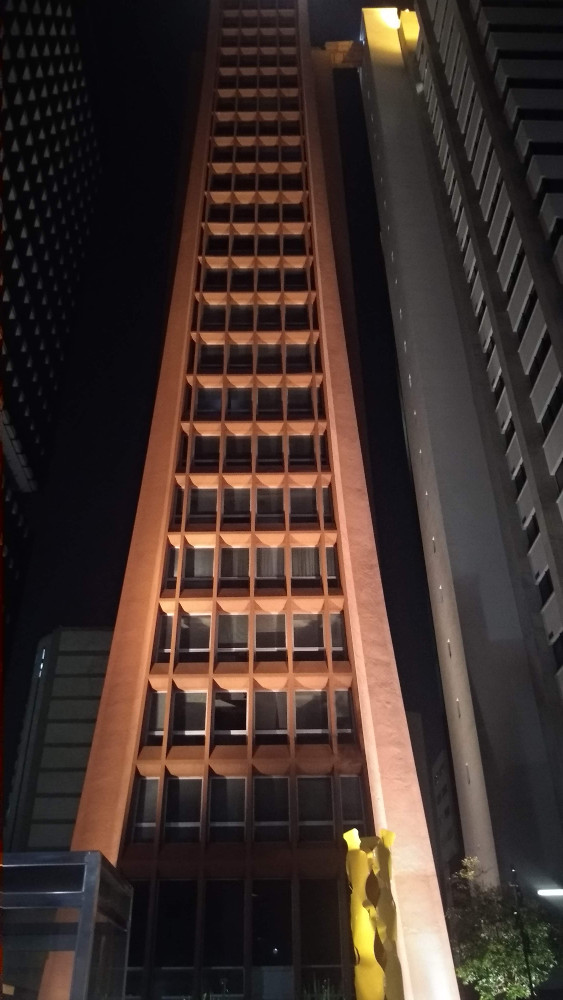
\includegraphics[scale=0.17]{paul}}
\end{picture}
  \affiliation{\tiny Instituto de Física\\
Universidad de Antioquia\\
Phenomenology Group}%
{http://gfif.udea.edu.co}%
{}%
{pixel}% small image here, use pixel for nothing
{}
\arxiv{arXiv:1811.11927 [PRD], arXiv:1906.09685 [PRD] and arXiv:1909.09574 }
\collaborators{ Carlos Yaguna (UPTC), Julian Calle, Óscar Zapata, Andrés Rivera (UdeA),\\ Walter Tangarife (Loyola University Chicago) }
}

\date{\tiny Oct 16, 2019 - ICTP-SAIFR Program on Particle Physics

  [PDF: \url{http://bit.ly/darkictp}] } % (optional) \today
%{
\includegraphics[scale=0.3]{udea}}
\titlegraphic{\hfill
\includegraphics[height=1.5cm]{udea}}

%\subject{Talks}
% This is only inserted into the PDF information catalog. Can be left
% out. 


% If you have a file called "university-logo-filename.xxx", where xxx
% is a graphic format that can be processed by latex or pdflatex,
% resp., then you can add a logo as follows:

% \pgfdeclareimage[height=0.5cm]{university-logo}{university-logo-filename}
% \logo{\pgfuseimage{university-logo}}



% Delete this, if you do not want the table of contents to pop up at
% the beginning of each subsection:
%\AtBeginSubsection[]
%{
%  \begin{frame}<beamer>
%    \frametitle{Outline}
%    \tableofcontents[currentsection,currentsubsection]
%  \end{frame}
%}
\setbeamercolor{block title}{bg=black!90,fg=white}

\newcommand{\chml}[2]{$\underline{\text{#1\hspace{#2}}}$}
\begin{document}


%=============== 
\begin{comentar}
%===============  
%=============
\end{comentar}
%=============

\maketitle


%%%%%%%%%%%%%%%%%%%%%%%%%
\section{$\Lambda$CDM paradigm (with baryonic effects)}




\begin{frame}
      \begin{figure}
    \centering
    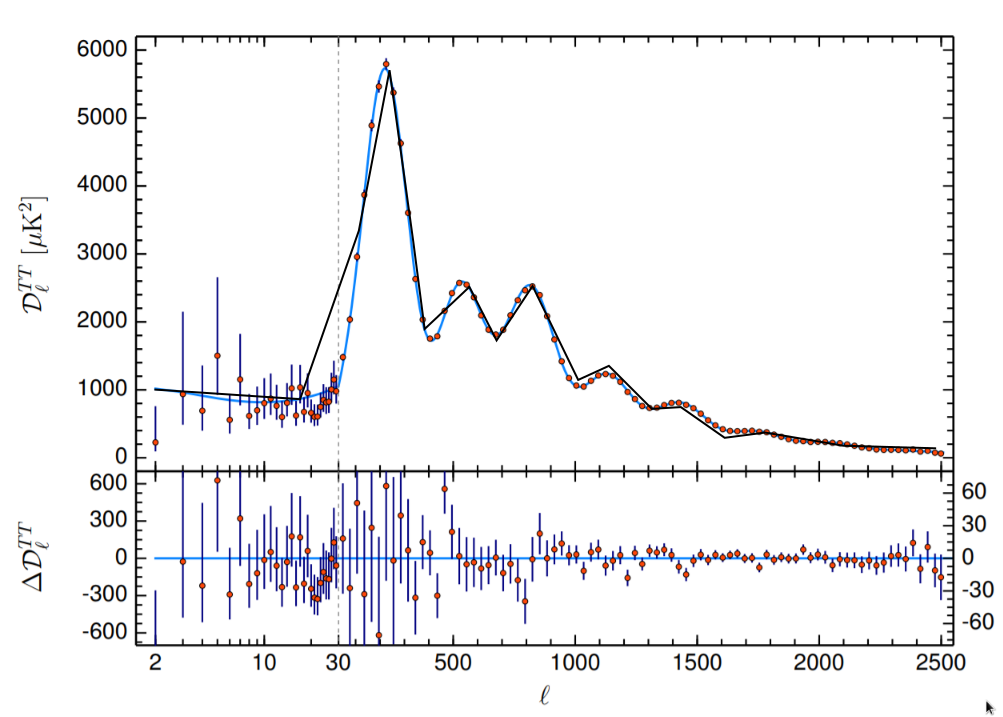
\includegraphics[scale=0.4]{planck2018}\\
     \tiny{Credit: Planck 2018}
  \end{figure}

% \small 
%   Why was the temperature of the CMB the same in all directions? \\
%   What was the origin of the small temperature fluctions?
  
\end{frame}



\begin{frame}
      \begin{figure}
    \centering
    \only<1>{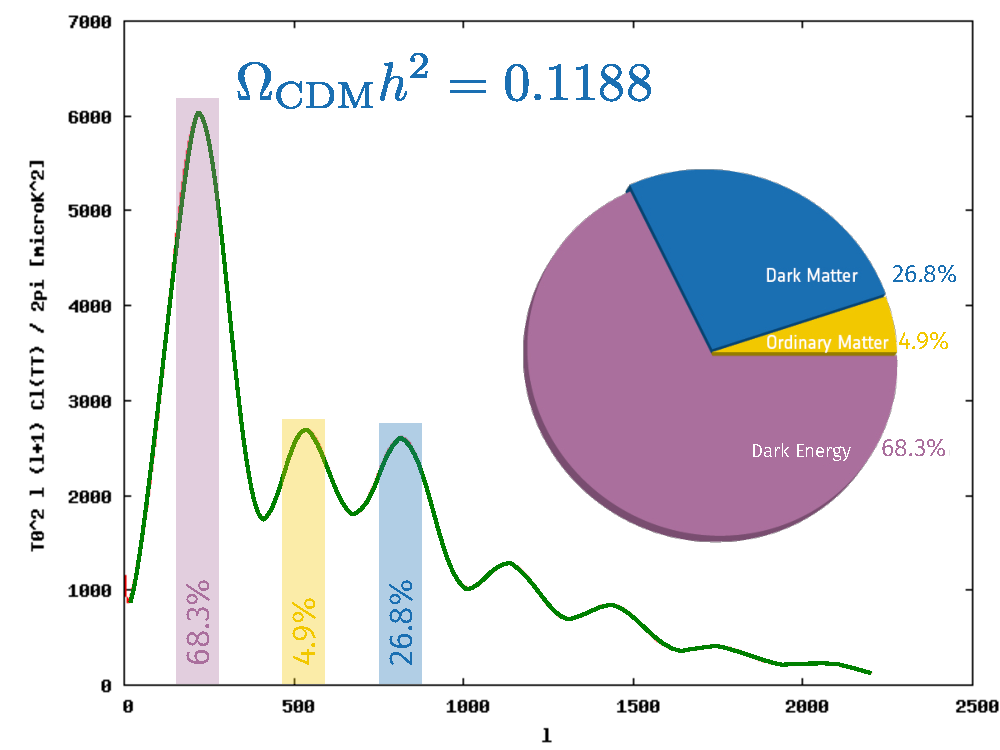
\includegraphics[scale=0.6]{cmbsoup0}}%
    \only<2>{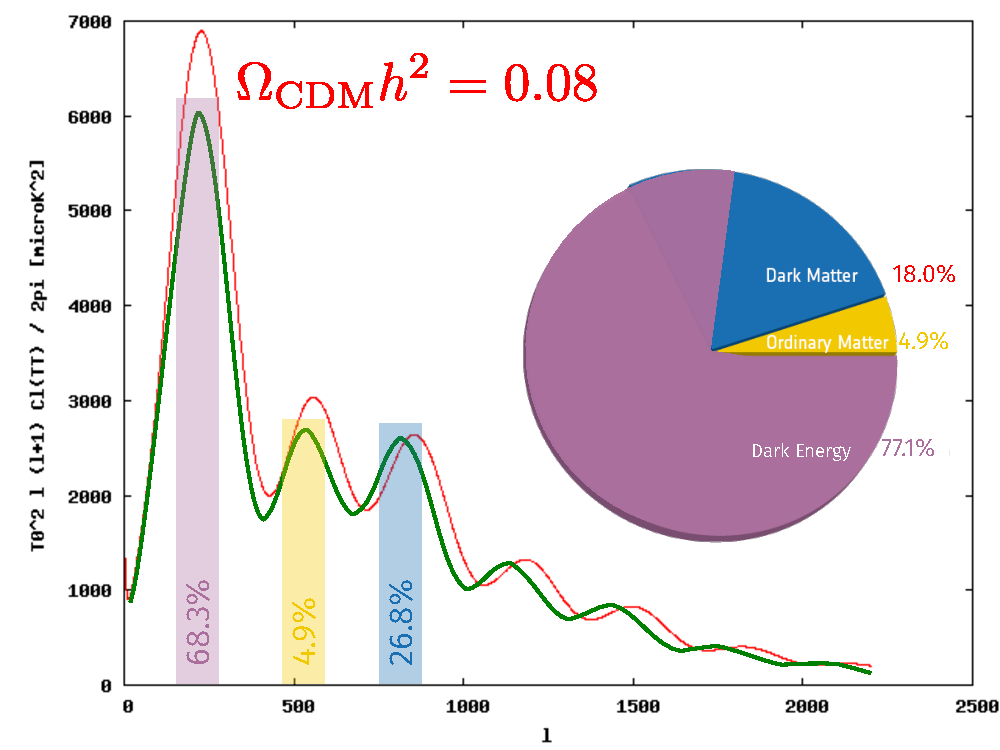
\includegraphics[scale=0.6]{cmbsoup1}}\\
     %\tiny{Credit: Planck 2018}
  \end{figure}
  
\end{frame}




\begin{frame}
\begin{picture}(320,250)  
  % \def\sdm{0.4}
  \only<1>{\put(35,-22){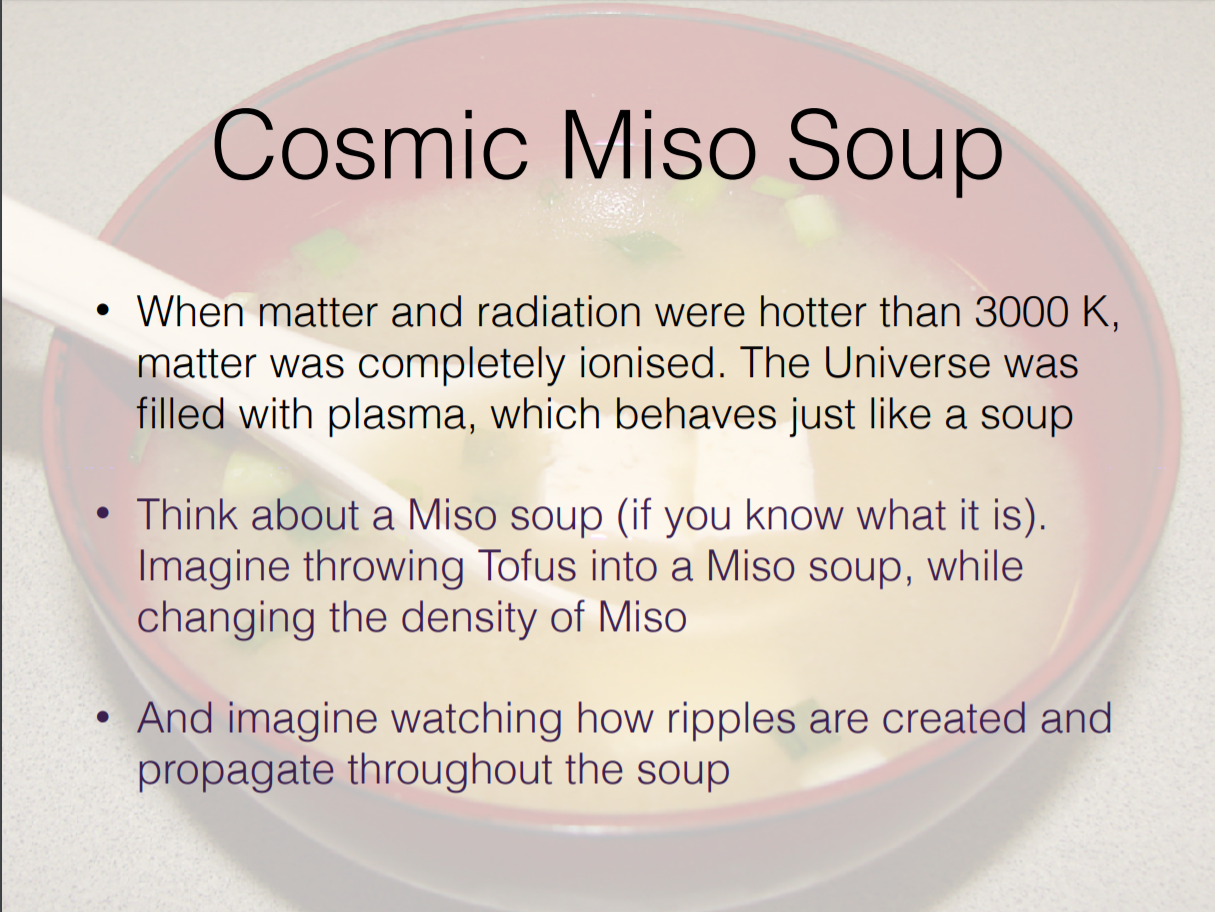
\includegraphics[height=\paperheight]{soup}}}%
  \only<2>{\put(35,-22){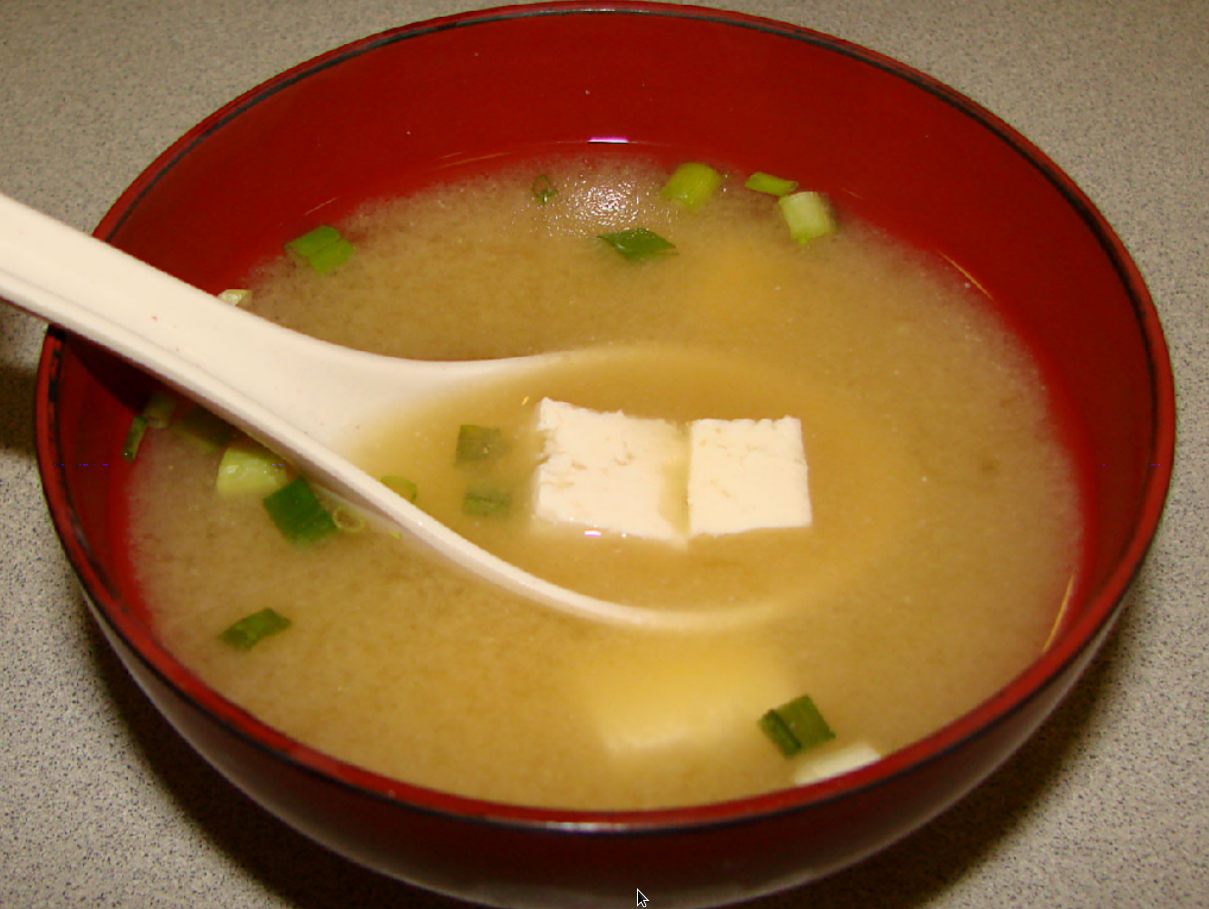
\includegraphics[height=\paperheight]{soup1}}}%
  \only<1->{\put(235, -15){{\tiny Credit: Komatsu, ICTP Summer School on Cosmology 2018 {\tiny (Video avalaible)}}}}%  
%    \only<1>{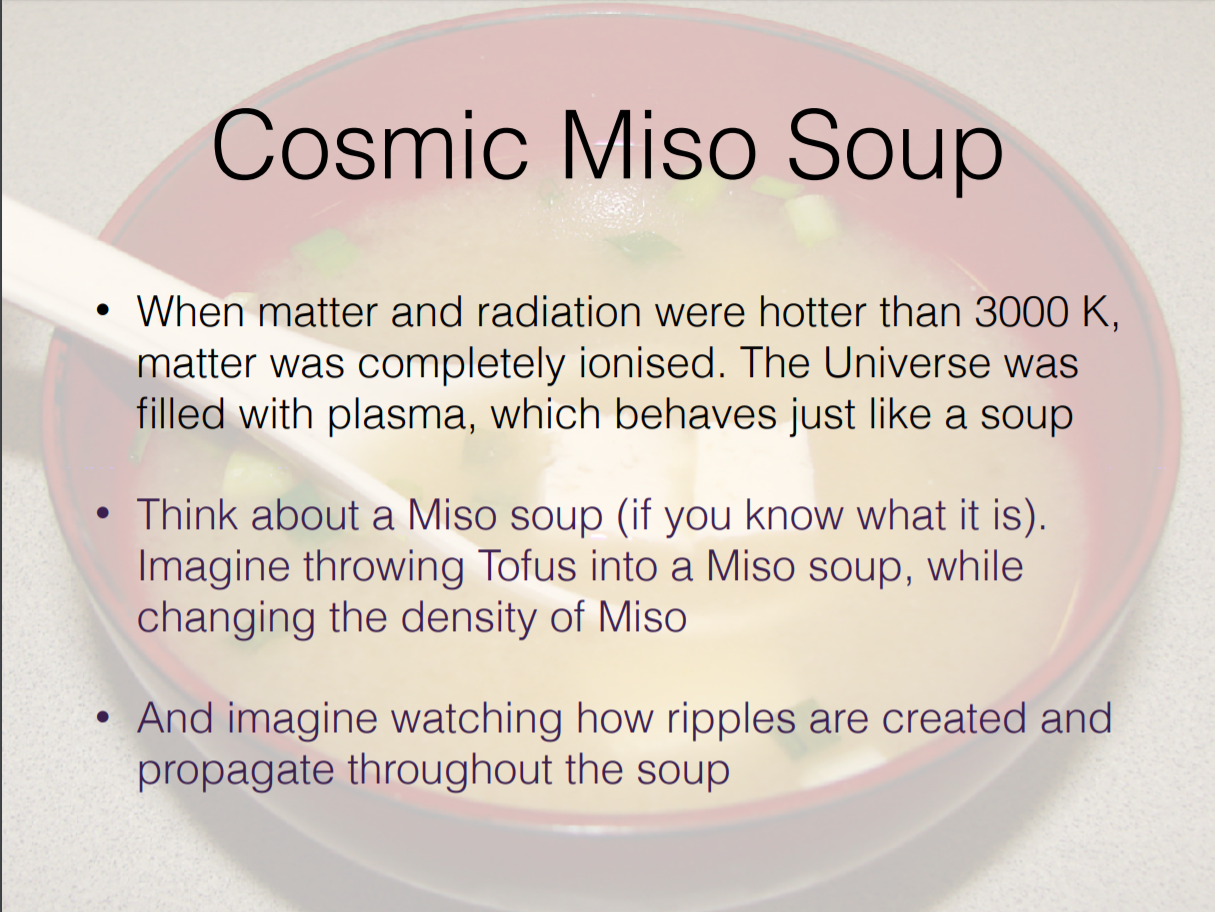
\includegraphics[scale=\sdm]{soup}}%
%    \only<2>{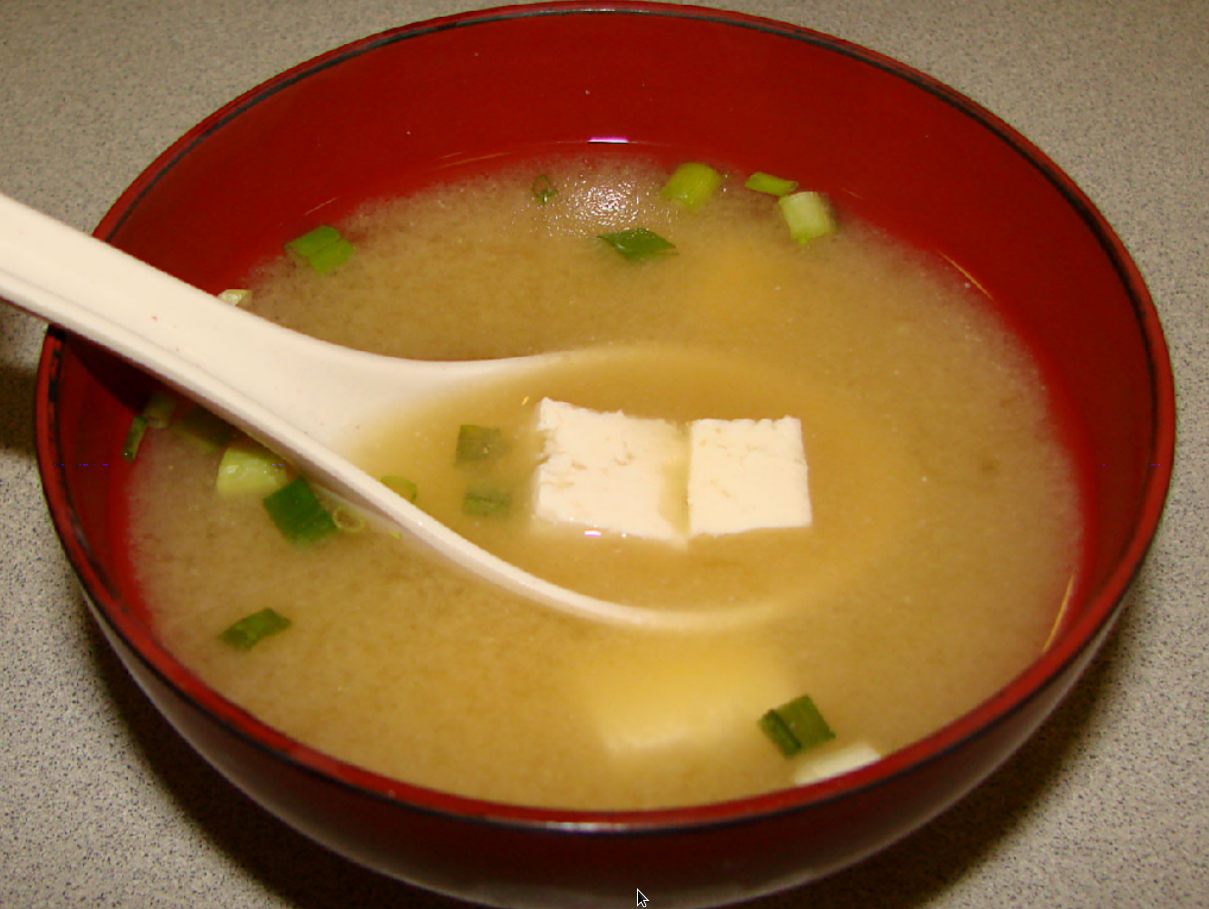
\includegraphics[scale=\sdm]{soup1}}\\
%    \only<1->
\end{picture}

\end{frame}



\begin{frame}
  \frametitle{Dark matter simulations}
  \begin{figure}
    \centering
    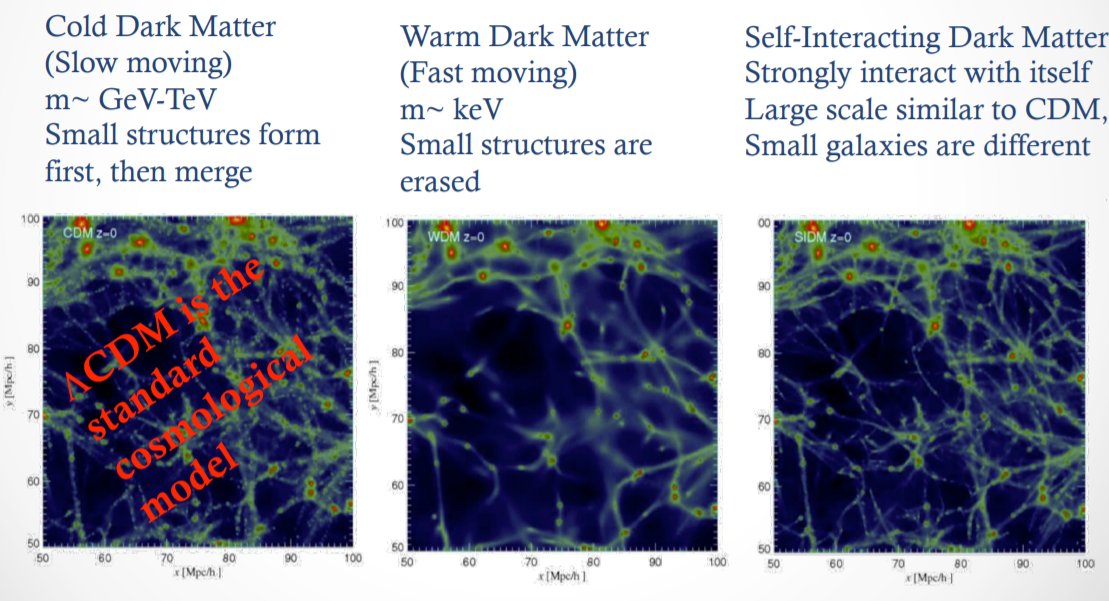
\includegraphics[scale=0.3]{dmtypes}\\
    {\tiny Credit: Arianna Di Cintio (Conference on Shedding Light on the Dark Universe with Extremely Large Telescopes, ICTP - 2018)}
  \end{figure}
\end{frame}


\begin{frame}
  \frametitle{Baryonic effects}
  \begin{figure}
    \centering
    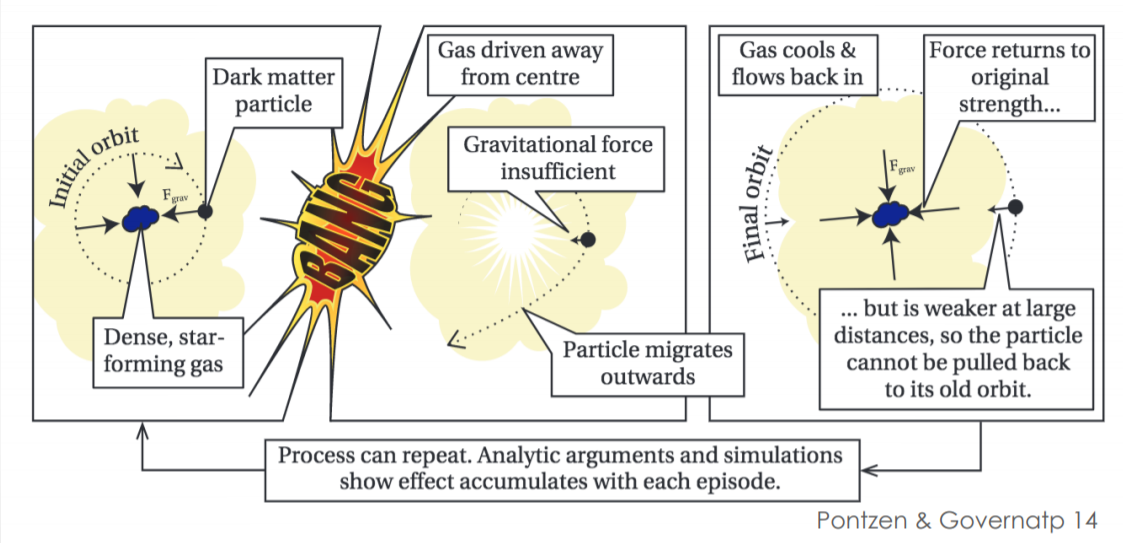
\includegraphics[scale=0.3]{snbang}
  \end{figure}
  Once the effect of baryonic physics is included, it is
  hard to distinguish between WDM/SIDM/CDM

  \begin{center}
    	
\footnotesize See: Gravitational probes of dark matter physics, M.R. Buckley, A.H.G. Peter, arxiv:1712.06615 [PR]
  \end{center}
\end{frame}

\begin{frame}
  \frametitle{Goal}
  \begin{columns}
  \begin{column}{0.65\textwidth}
  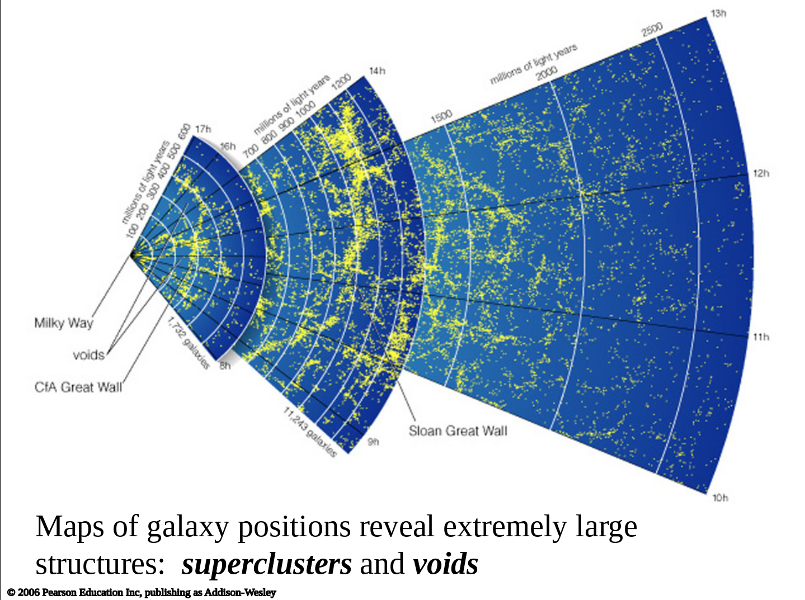
\includegraphics[scale=0.35]{galaxsmall}     
  \end{column}
  \begin{column}{0.35\textwidth}
    The DESI experiment\\
    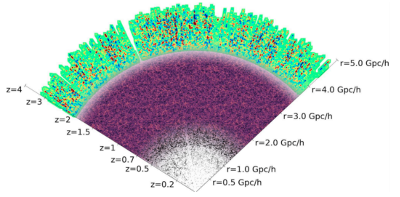
\includegraphics[scale=0.43]{DESIsmall}
    
    {\tiny Credits: J. Forero \url{http://cosmology.univalle.edu.co/} }
  \end{column}
\end{columns}

  %\vspace{-0.3cm}

\end{frame}


\begin{frame}
  \frametitle{Cosmic web}

      Dark matter in the universe evolves through gravity to form a complex network
      of halos, filaments, sheets and voids, that is known as the cosmic web

      {\tiny A.C Rodriguez \emph{et al} arXiv:1801.09070 [CAC]}

    Cosmological simulations of structure formation predict that the
    majority of gas in the intergalactic medium (IGM) is distributed
    in a cosmic web of sheets and filaments as a consequence of
    gravitational collapse.  The intersections of these structures
    become the locations at which galaxies and their supermassive
    black holes (SMBHs) form and evolve.

    [...] at a $z$ of $\sim 3$, $>60\%$ of all gas in the
    Universe resides in filaments
    
    {\tiny H. Umehata \emph{et al}, Science  \textbf{366}, 97, 4 Oct 2019}

% Read more at: 

%   \frametitle{General considerations}
%   \note{From doi:  [10.1098/rsta.2009.0209]
%     We live in an exciting, if somewhat bewildering, time in terms of our understanding of the Universe. The concept of dark matter, as a significant component of the Universe, dates back to the 1970s following the realization that most galaxies are surrounded by unseen haloes. The null results of the Galactic microlensing surveys and the abundance of light elements produced in the big bang further suggest that dark matter is non-baryonic in form. Structure formation models can account for the presently observed large-scale distribution of galaxies if this non-baryonic matter is made of massive non-relativistic (i.e. ‘cold’) particles. Despite this progress, after 40 years, we have yet to detect the dark matter particle itself. Given how both strong and weak gravitational lensing have, in barely a decade, considerably added to our knowledge of the distribution and amount of dark matter, it is relevant to ask what these techniques can offer in the future.}

%   \note{Astronomical observations can define the spatial distribution of dark matter from small to large scales. Theory predicts this distribution in terms of the spectrum of physical scales over which the density of dark matter fluctuates. }
\end{frame}


\begin{frame}
  \frametitle{Cooking the soup: Cosmic web}
  \begin{quote}
    Dark matter connects clusters of galaxies with massive tendrils, forming a cosmic web that serves as an unseen skeleton for the universe.

\vspace{-0.3cm}    
    {\tiny \url{https://phys.org/news/2018-06-years-scientists-account-universe.html}}

    
  \end{quote}

\def\heifig{4.8cm}
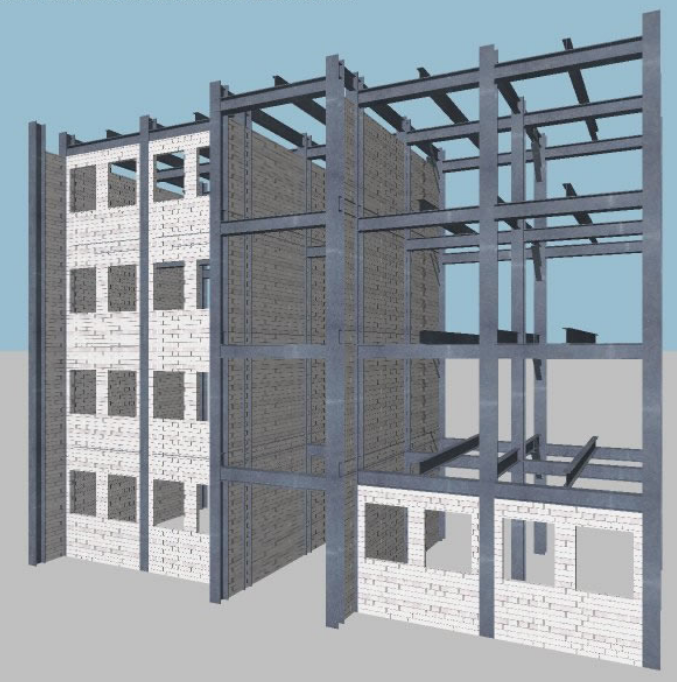
\includegraphics[height=\heifig]{building} \hspace{2cm}\only<1>{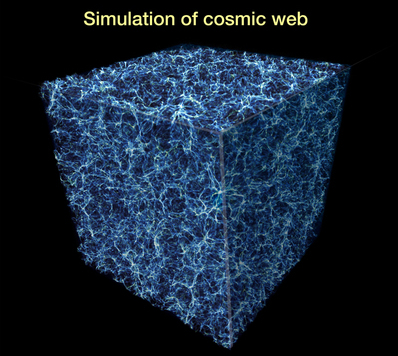
\includegraphics[height=\heifig]{lowweb}}\only<2>{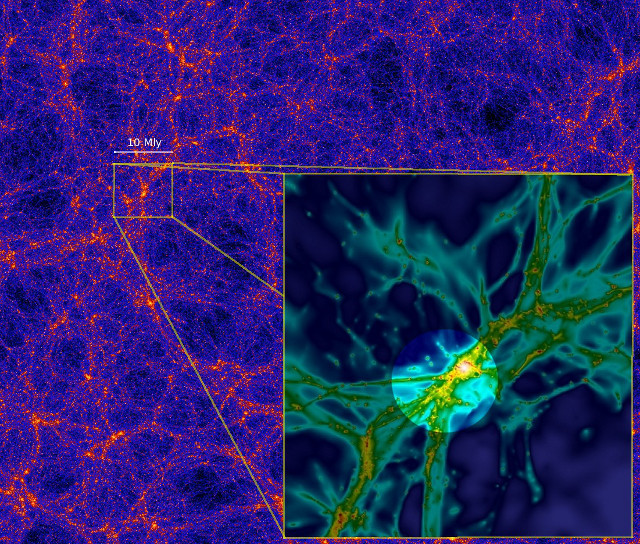
\includegraphics[height=\heifig]{cosmic_web_simulation}}

  % \begin{figure}
  %   \centering
  %   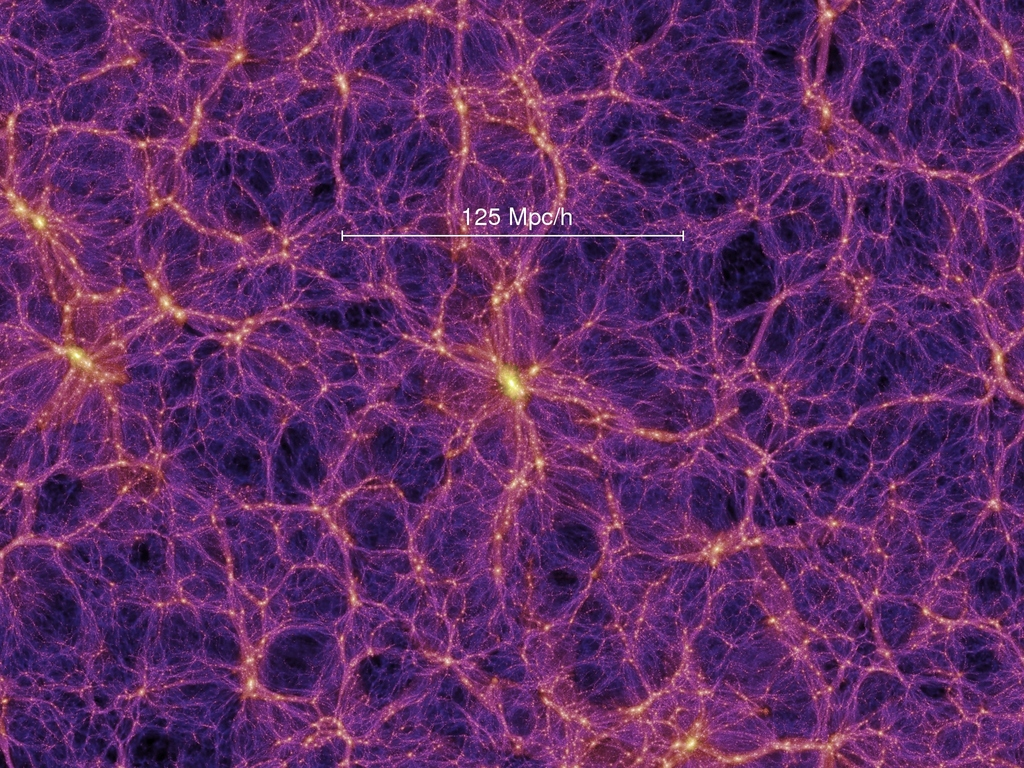
\includegraphics[scale=0.2]{cosmic-web}\\
  %   {\tiny Milenium simulation: \url{https://wwwmpa.mpa-garching.mpg.de/galform/virgo/millennium/}}
  % \end{figure}

\begin{block}{An excess of a gas is observed between Milky Way and Andromeda}
  \scriptsize These great filaments are made largely of \alert{dark matter} located in the space between galaxies\\ and filled with $60\%$ of the \alert{primordial gas!} \hfill\only<1>{{[\url{https://hubblesite.org}]}}
  \end{block}
\end{frame}


% % \begin{frame}
% %   \frametitle{Cosmic Anatomy}
% %   \def\sana{0.8cm}
% %   \centering
% %   { \tiny Baryons \hspace{\sana} Missing Baryons \hspace{\sana} Dark Matter}
% %   \begin{figure}
% %     \centering
% %     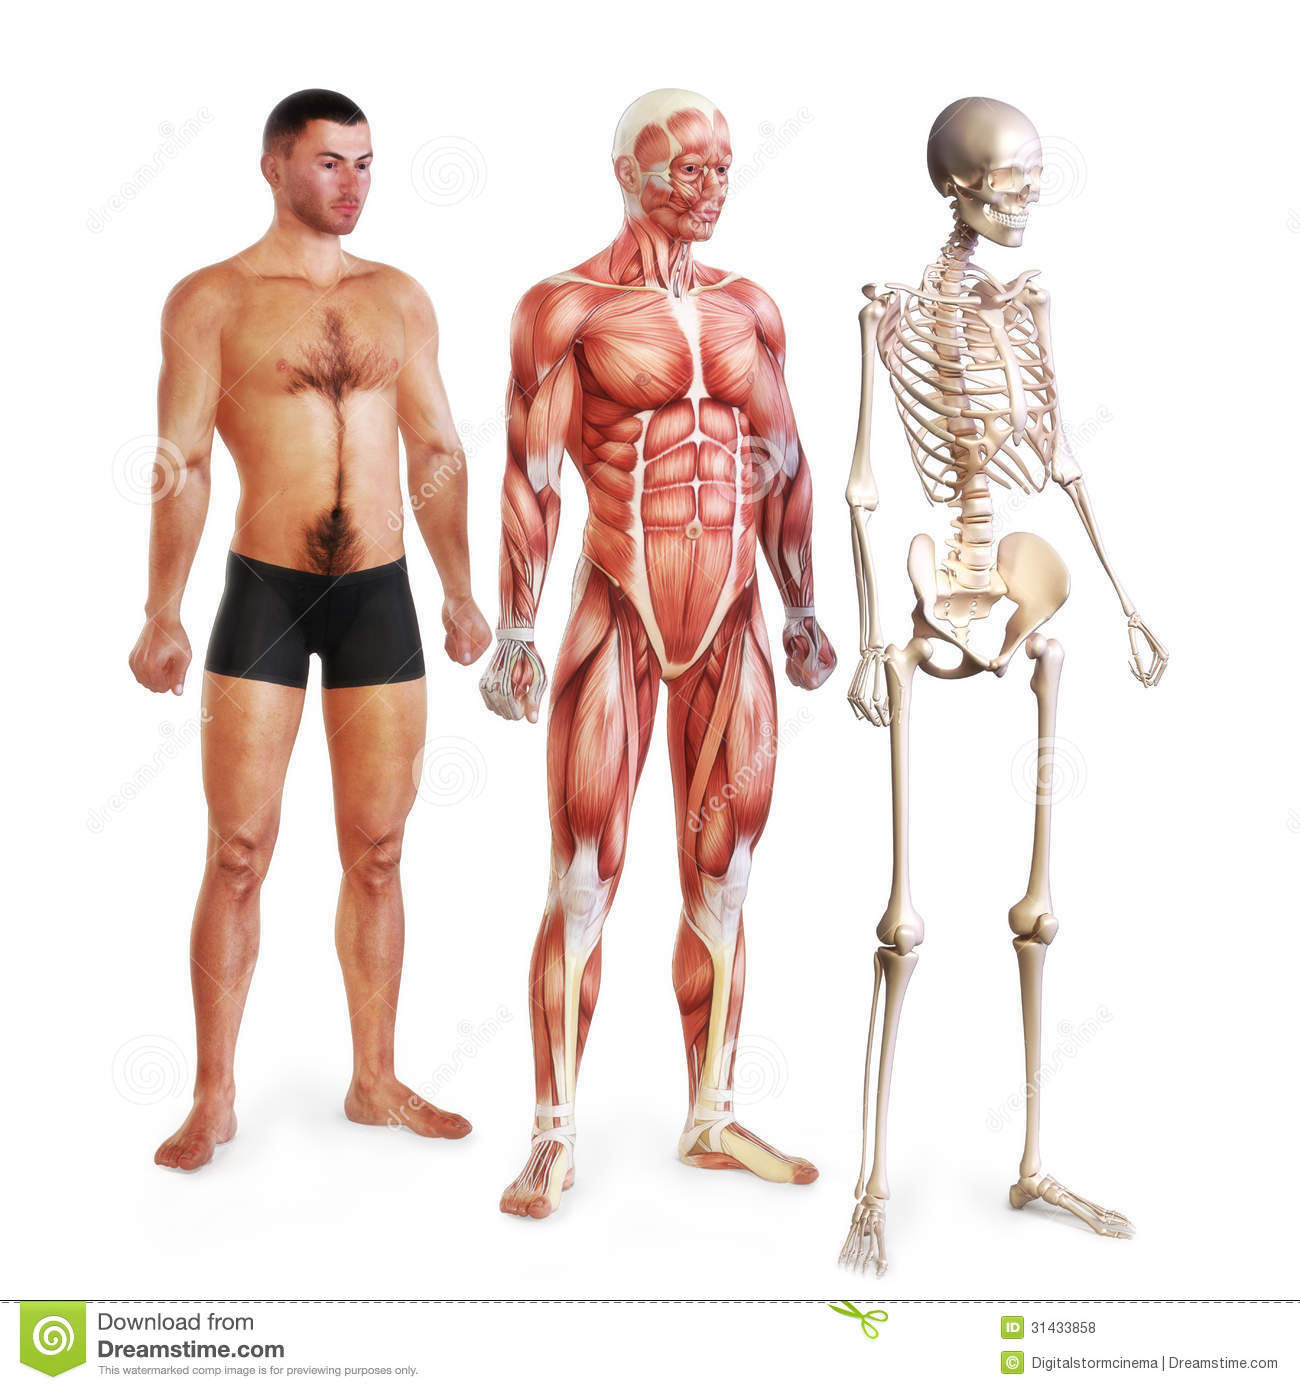
\includegraphics[scale=0.6]{anatomy}\\
% %   \end{figure}
% % \end{frame}


% % \begin{frame}
% %     \frametitle{The muscles}
% % \begin{figure}
% %   \centering
% %   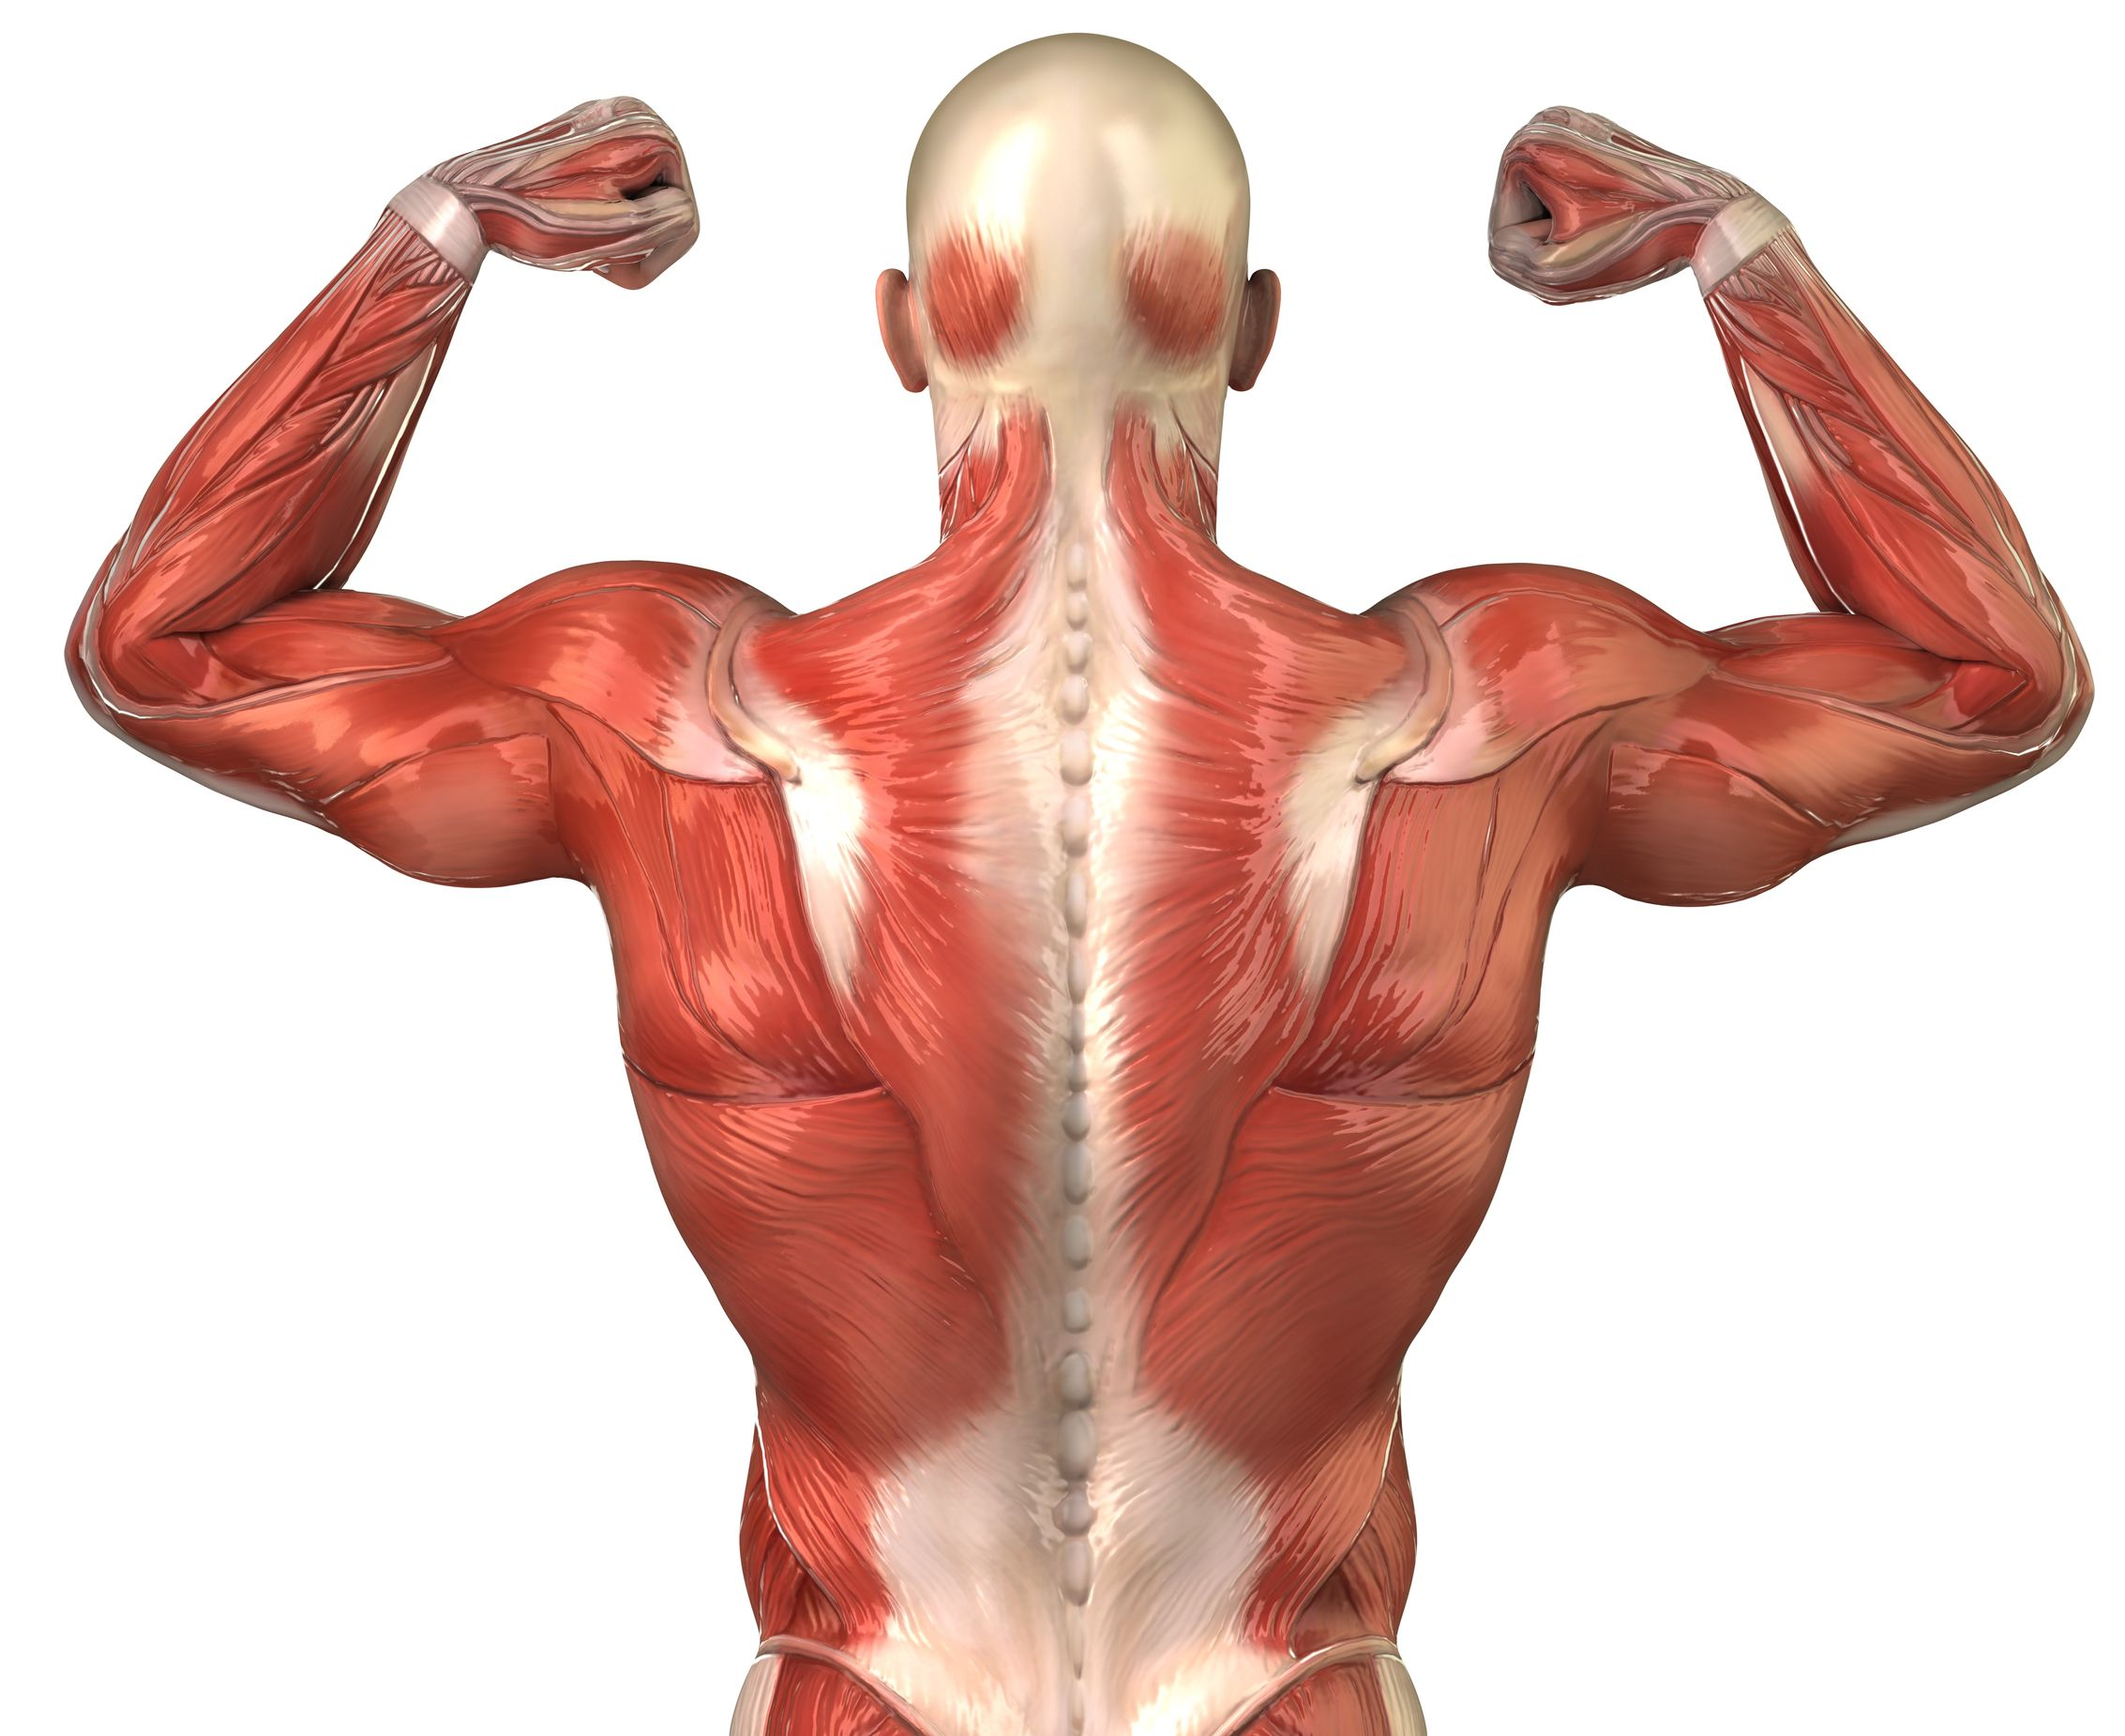
\includegraphics[scale=0.5]{muscles-anatomy-back}\\
% %   {\tiny Credit: \url{http://sciencedrivennutrition.com}}
% % \end{figure}
% % \end{frame}

\begin{frame}
  \frametitle{Direct observations of filaments}
  \small
  \textbf{Where are the Baryons?} (Cen, Ostriker, astro-ph/9806281 [AJ])
  \begin{quote}
   \scriptsize Thus, not only is the universe dominated by dark matter, but more than one half of the normal matter is yet to be detected. (the muscles)
  \end{quote}

  \vspace{-0.5cm}

\begin{columns}
  \begin{column}{0.48\textwidth}
\begin{figure}
  \centering
  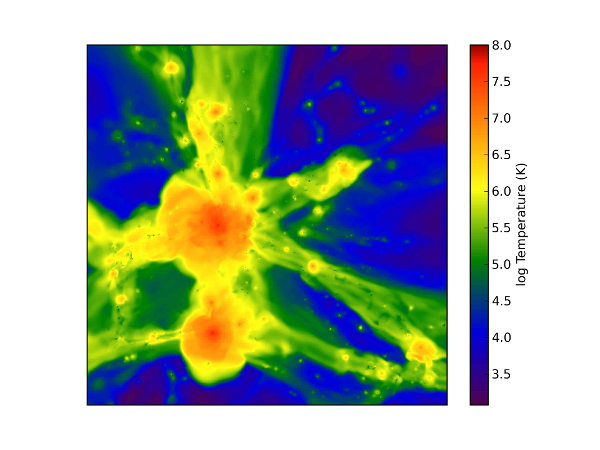
\includegraphics[scale=1.4]{clusterboXsmall}\\
  {\tiny Credit: Cen, arXiv:1112.4527 [AJ]}
\end{figure}

  \end{column}
  \begin{column}{0.48\textwidth}
    \scriptsize
    Warm-hot intergalactic medium (WHIM)

    Density-weighted temperature projection of a portion of the refinement box of the C run of size  $\left(18\,h^{-1}\text{Mpc} \right)^3$.

    Low temperature WHIM confirmed by O VI line that peak at $T\sim 3\times 10^5\ \text{K}$
  \end{column}
\end{columns}

\small   

\includegraphics[scale=0.1]{new}Hotter phases of the WHIM: \textbf{  Observations of the missing baryons in the warm-hot intergalactic medium}
  (Nicastro, \emph{et al.} arXiv:1806.08395 [Nature]). 

\end{frame}


% umerical simulations in the framework of the commonly accepted (ΛCDM) cosmological paradigm predict that, starting at a redshift of $z\approx 2$ and during the continuous process of structure formation, diffuse baryons in the intergalactic medium (IGM) condense into a filamen-tary web (with electron densities of $n_e\approx 10^{-6}-10^{-4}\ \text{cm}^{-3}$ and undergo shocks that heat them up to temperatures of $T\approx 10^5-10^7\ \text{K}$, making the by-far-largest constituent of the IGM, hydrogen, mostly ionized. At the same time, galactic outflows powered by stellar and active galactic nucleus (AGN) feedback enrich the IGM baryons with metal. How far from galaxies these metals roam depends on the energetics of these winds, but it is expected that metals and galaxies are spatially correlated.
  
  %     \begin{quote}
  % From: \url{https://phys.org/news/2018-06-years-scientists-account-universe.html}

  %   The scientists used the European Space Agency's XMM-Newton X-ray space telescope to study the BL Lacertae quasar 1ES 1553+113, an active, supermassive black hole at the center of a galaxy. Quasars gobble up matter and shine brightly in many wavelengths of light, from radio waves to X-rays. These celestial lighthouses can basically back light the material that crosses the beam's path, just as a flashlight beam illuminates unseen motes of dust in the air.
  % \end{quote}

  % \begin{quote}

  %   Studying the chemical fingerprint of oxygen in the X-rays from the quasar light, the scientists found a large amount of extremely hot intergalactic gas so much that they calculate that this gas could account for up to 40 percent of the baryonic matter in the cosmos, which could be enough to explain the missing matter.

  % \end{quote}

  % \begin{quote}

  %   Taotao Fang of the Jiujiang Research Institute in China, who was not involved in the study, pointed to a few possible alternate explanations, including that the ionized gas signal may have come from within a galaxy rather than from intergalactic gas embedded in a dark matter filament.
  % \end{quote}
  



% \begin{frame}
%     \frametitle{The skeleton}
% \begin{figure}
%   \centering
%   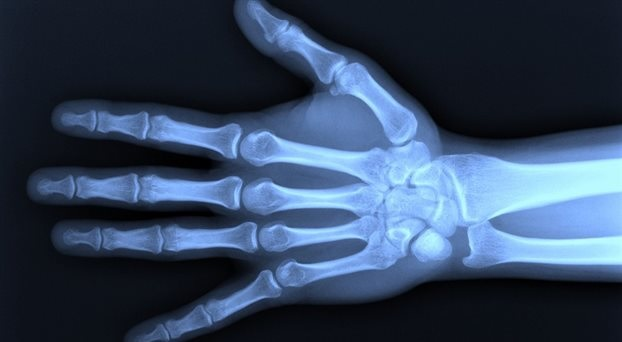
\includegraphics[scale=0.5]{xray}\\
%   {\tiny Credit: \url{https://www.disnola.com}}
% \end{figure}
% \end{frame}







% From: \url{http://www2.cnrs.fr/en/1247.htm},  
% \begin{quote}
%   the MegaCam, which has 340 megapixels, using a technique known as  “This technique works somewhat like an X-ray,” says Kilbinger. “You can’t see inside the human body, and we can’t see the dark matter directly.” Dark matter is dark, but any light emitted from galaxies must pass around it, and the diversion is recorded as a gravitational distortion. Astronomers can then use this gravitational imprint to calculate the size of the matter that caused it. Using such techniques, astronomers estimate that dark matter forms web-like structures, made up of clusters, filaments, and large rope-like structures that the new research has uncovered. But only until dark matter becomes visible will these assumptions become fact. Nonetheless, the new findings open up a dizzying vista of possibility, where, with better telescopes in the future, more precise lay-out and details of dark matter could be revealed. Understanding the formation of dark matter could help scientists improve their knowledge on how the universe evolved, and what its future might be. “There are other techniques that can measure dark matter,” says Kilbinger, “but over the next 10 to 20 years, I think this one will become the most used. And that’s why people are so excited about it.”
% \end{quote}


% From:
% \begin{quote}
%   Looking deep into space, and literally peering back in time, is like experiencing the universe in a house of mirrors where everything is distorted through a phenomenon called gravitational lensing. 
% \end{quote}



% coupled with the angular resolution of ELTs this will open a unique window to constrain the
% dark matter properties with detail and statistical completeness. 










% \begin{frame}
%   \frametitle{Evidences at all redshifts.}
% \begin{columns}
%   \begin{column}{0.48\textwidth}
%       \begin{itemize}
%   \item   For cluster of Galaxies
%   \item For stars inside Galaxies
%   \item Inside our Galaxy
%   \item Senatore reconstruction
%   \item En las simulaciones se parte de la CMB
%   \end{itemize}
%   \end{column}
%   \begin{column}{0.48\textwidth}

%       \begin{figure}
%     \centering
%     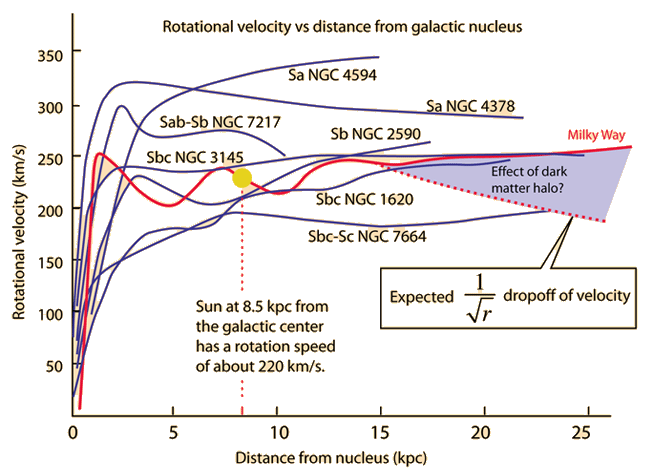
\includegraphics[scale=0.2]{gallightcrv}
%   \end{figure}

%   \end{column}
% \end{columns}

% \end{frame}



% \begin{frame}
%   \frametitle{Inner Milky Way}
%   \url{https://www.nature.com/articles/nphys3237}
% \end{frame}

\begin{frame}
  \frametitle{A filament of dark matter between two clusters of galaxies}
  \begin{columns}
  \begin{column}{0.45\textwidth}
  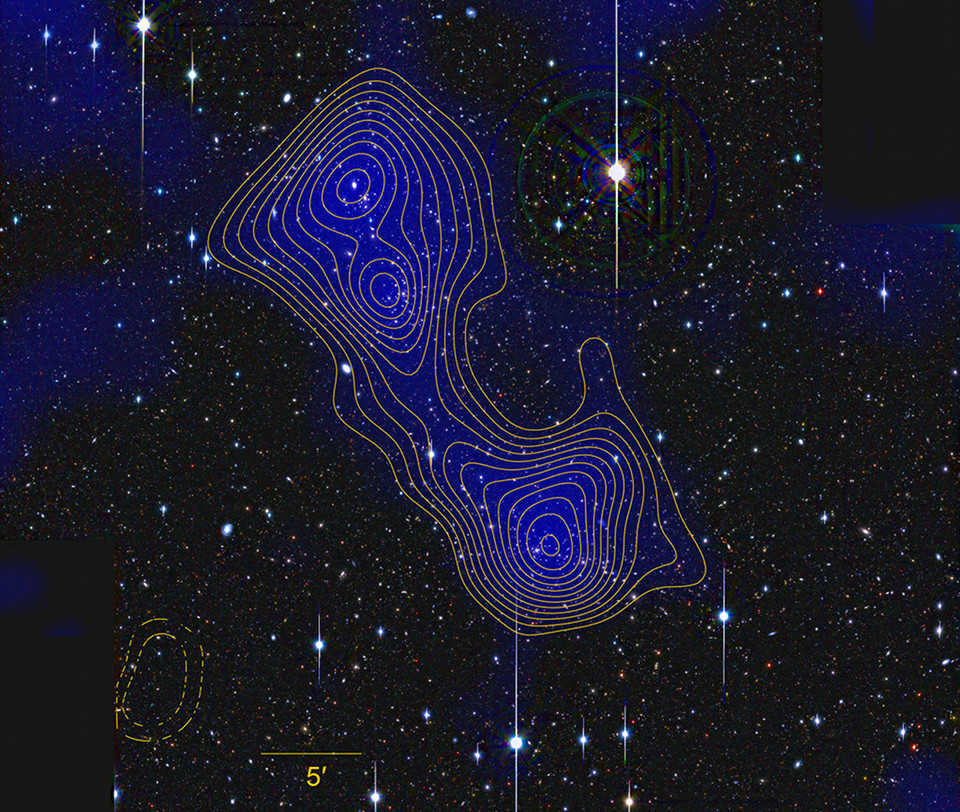
\includegraphics[height=6cm]{A222+3_mass}
  \end{column}
  \begin{column}{0.55\textwidth}
%It is a firm prediction of the concordance Cold Dark Matter (CDM) cosmological model that
%galaxy clusters live at the intersection of large-scale structure filaments

    \begin{block}{Supercluster
system of three galaxy clusters}
    \begin{itemize}
    \item Abell 222 (south) detected at $\sim 8\sigma$
    \item Abell 223 (north) double galaxy cluster seen at $\sim 7\sigma$   
    \end{itemize}

    \end{block}



  \fcolorbox{blue}{blue}{\color{white}reconstructed surface mass density (blue)}
  
  \fcolorbox{Yellow}{white}{significance contours from $0.5\sigma$ to $2.5\sigma$}


    {\tiny J.P. Dietrich \emph{et al}, arXiv:1207.0809 [Nature]}

   {\tiny For a recent review see: arXiv:1905.08991}  
  \end{column}
  \end{columns}

\end{frame}

\begin{frame}
  \frametitle{Three-dimensional pictures of Ly$\alpha$ filaments}
  \begin{columns}
  \begin{column}{0.5\textwidth}
  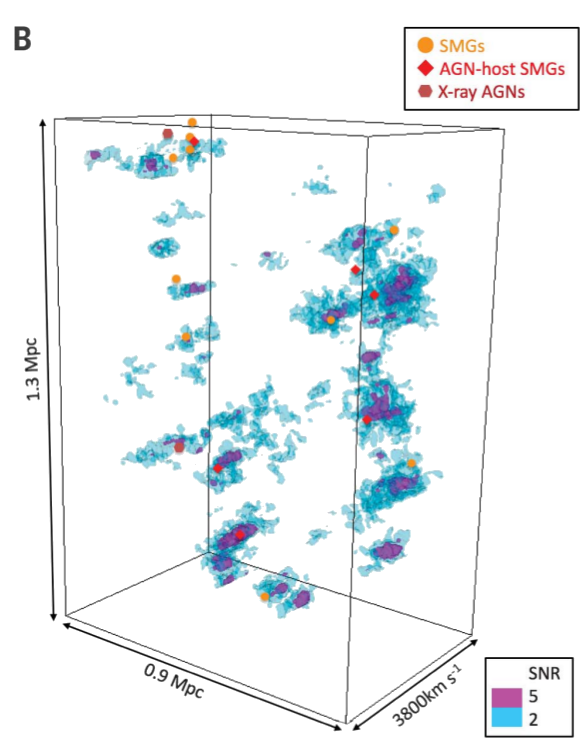
\includegraphics[scale=0.3]{fila}
  \end{column}
  \begin{column}{0.5\textwidth}
  The 3D distribution of
  Ly$\alpha$ filaments shown with

  \fcolorbox{magenta}{magenta}{signal-to-noise ratio (SNR) > 5}
  
  \fcolorbox{cyan}{cyan}{signal-to-noise ratio (SNR) > 2}


    {\tiny H. Umehata \emph{et al}, Science  \textbf{366}, 97, \alert{4 Oct 2019}}

  \end{column}
  \end{columns}

\end{frame}
%%%%%%%%%%

\begin{frame}
  
  \begin{block}{Dark matter properties}
      \begin{quote}
    Apart from its manifold gravitational influences, (\alert{particle}) dark matter has so far eluded detection,
prompting model builders to think more broadly about what dark matter can be and in
the process consider other and more subtle ways to search for it.

\hfill{\tiny Agrawal, \emph{et al}, \arXiv{1610.04611} [JCAP]}
\end{quote}
\end{block}

\end{frame}

\section{Dark sectors}




\section{Dark sectors}




\begin{frame}
\begin{picture}(320,250)
\only<1->{\put(-24,-22){\begin{overpic}[scale=0.352]{z2_bkg}\end{overpic}}}%
\only<1>{\put(194,92){\begin{overpic}[scale=0.2]{infinity}\end{overpic}}}%
\only<1->{\put(30,160.5){ $\mathbf{SM}$  }}%
\only<1->{\put(18,115){\begin{overpic}[scale=0.118]{smfp}\end{overpic}}}%
\only<2>{\put(204,158){ \begin{overpic}[scale=0.27]{dfdz}\end{overpic}}}%
% \only<2>{\put(224,195){ {\huge \only<2>{
%         \hspace{0.4cm}\begin{minipage}{3cm}
%                     Hidden \\
%           QED
%         \end{minipage}
%       }}  }}%
\only<3->{\put(250,180){\Large $\color{red}\mathcal{L}=-\frac{1}{4}V_{\mu\nu}V^{\mu\nu}+i \overline{\psi}\cancel{\mathcal{D}} \psi-m \overline{\psi}\psi,. $   }}%
\only<3->{\put(280,218.5){ \Huge {{\color{red}Lo}{\color{red}cal}} $\color{red}U(1)_{\mathcal{D}}$  }}%
\only<3->{\put(280,150){
    {\color{red}Relic abundance}
    $\color{red} \psi\overline{\psi}\to \gamma_{\mathcal{D}}\gamma_{\mathcal{D}}$  
  }}%
\only<3->{\put(160,120){\Large $F_{\mu\nu}{\color{red}\ V^{\mu\nu}} $   }}%
\only<3->{\put(204,0){ \begin{overpic}[scale=0.2]{tcdm1}\end{overpic}}}%

\only<4->{\put(280,0){ \begin{overpic}[scale=0.27]{alert}\end{overpic}}}%
\only<4->{\put(296,40){ {\huge 
        \hspace{0.4cm}\begin{minipage}{3cm}
          Too\\

          \vspace{-1.4cm}
          Restricted
        \end{minipage}
      }  }}%
\end{picture}
\end{frame}

\begin{frame}%[fragile,allowframebreaks]
\frametitle{Explain also small neutrino masses }
  In the following discussion we use the following doublets 
\begin{align}
  H=&
  \begin{pmatrix}
    H^+\\
    H^0
  \end{pmatrix},&
  L_i=&
  \begin{pmatrix}
    \nu_{Li}\\
    e_{Li}^{-}
  \end{pmatrix}.
\end{align}
corresponding to the Higgs doublet and the lepton doublets (in Weyl Notation) respectively, such that
\begin{align*}
  L_i\cdot H=&\epsilon_{ab}L_i^a H^b\,,& a,b=&1,2
\end{align*}

\end{frame}


\begin{frame}
  \frametitle{Standard model extended with $\operatorname{U}(1)_X$ gauge symmetry}
  \begin{table}
    \centering
        \rowcolors{1}{RoyalBlue!20}{}
  \begin{tabular}{c|c|c|c}
    \hline  
    Fields     & $\operatorname{SU}(2)_L$ & $\operatorname{U}(1)_Y $ & $\operatorname{U}(1)_{X}$\\ \hline
$L $    & $\boldsymbol{2}$& $-1/2$  &  $\color{blue}l$ \\
$Q $    & $\boldsymbol{2}$& $-1/6$  &  $q$   \\
$d_R $  & $\boldsymbol{1}$& $-1/2$  &  $d$ \\
$u_R $  & $\boldsymbol{1}$& $+2/3$  &  $u$\\
$e_R $  & $\boldsymbol{1}$& $-1$    &  $e$   \\
$H $    & $\boldsymbol{2}$& $-1/2$  &  $h$   \\
$\psi $ & $\boldsymbol{1}$& $0$     &  $n$   \\
  \end{tabular}
  \caption{The new  and fermions with their respective charges. }
    \label{tab:partcont2}
\end{table}


\end{frame}



\begin{frame}
  \frametitle{One parameter $\operatorname{U}(1)_X$ SM extension }
        \rowcolors{1}{RoyalBlue!20}{}
  \begin{tabular}{c|c|c|c|c|c|c|c||c}
    \hline  
    Fields     & $\operatorname{SU}(2)_L$ & $\operatorname{U}(1)_Y $ & $\operatorname{U}(1)_{X}$& $\color{red}\operatorname{U}(1)_{B-L}$& $\operatorname{U}(1)_R$& $\operatorname{U}(1)_D$& $\operatorname{U}(1)_G$ & $\operatorname{U}(1)_{\mathcal{D}}^{{\color{Yellow}*}}$\\ \hline
$L $  & $\boldsymbol{2}$& $-1/2$  &  ${\color{blue}l}      $&  $\color{red}-1$&    $0$ &  $-3/2$     &  $-1/2$&$0$ \\    
$Q $  & $\boldsymbol{2}$& $-1/6$  &  $-{\color{blue}l}/3   $& $\color{red}1/3$&    $0$&  $1/2$    &  $1/6 $&$0$ \\
$d_R $& $\boldsymbol{1}$& $-1/2$  &  $1+2{\color{blue}l}/3 $&  $\color{red}1/3$&    $1$&  $0$ &  $2/3 $&$0$ \\
$u_R $& $\boldsymbol{1}$& $+2/3$  &  $-1-4{\color{blue}l}/3$&  $\color{red}1/3$&   $-1$&  $1$&  $-1/3$&$0$ \\
$e_R $& $\boldsymbol{1}$& $-1$    &  $1+2{\color{blue}l}   $&  $\color{red}-1$&    $1$ &  $-2$    &  $0   $&$0$ \\
$H $  & $\boldsymbol{2}$& $1/2$  &   $-1-{\color{blue}l}   $&  $\color{red}0$&    $-1$ &  $1/2$   &  $-1/2$&$0$ \\\hline
%$S$ & $\boldsymbol{1}$ & $0$  & $ 2 \psi_N$& $\color{red}2 \psi_N$&  $2 \psi_N$ & $2 \psi_N$& $2 \psi_N$ &$0$ \\
 $\sum_\alpha n_{\alpha}$ & $\boldsymbol{1}$ & $0$ & $-3$& $\color{red}-3$&  $-3$ & $-3$& $-3$&$0$\\
 $\sum_\alpha n_{\alpha}^{3}$ & $\boldsymbol{1}$ & $0$ & $-3$& $\color{red}-3$&  $-3$ & $-3$& $-3$&$0$\\ \hline
  \end{tabular}

  % {\color{Yellow}*} Use vector like fermions $\mathcal{D}(\psi_L)=\mathcal{D}(\psi_R)\to n-n=0$
  
  % Solutions in terms of a parameter: arXiv:1811.11927, N. Okada, \emph{et al} [PRD];

  % and some specific examples from: arXiv:1705.05388,  Farinaldo Queiroz,  \emph{et al} [JHEP]

  % \alert{All known $\operatorname{U}(1)_{B-L}$ (radiative) neutrino solutions apply for $\operatorname{U}(1)_X$}:
\end{frame}

\begin{frame}
  \frametitle{solutions with $\sum n_{\alpha}=0 $ and $\sum n_{\alpha}^3=0 $}
\end{frame}

\begin{frame}
  \frametitle{\invisible<1>{Or$\cdots$ combine known} solutions \only<1>{with $\sum n_{\alpha}=-3$ and $\sum n_{\alpha}^3=-3$}\only<2>{with $\sum n_{\alpha}=0$ and $\sum n_{\alpha}^3=0$}}
  \vspace{-0.7cm}
\begin{columns}
  \begin{column}{0.52\textwidth}
    \begin{table}
  \centering
  \renewcommand{\arraystretch}{1.4}
      \rowcolors{1}{RoyalBlue!20}{}
  \begin{tabular}{c|l}\hline
$\left(\nu_{R1},\nu_{R2},\psi_{N-2},\cdots\right)$     & Ref \\ \hline
    $\left(-1,-1,-1\right)$&\tiny hep-ph/0611205, S. Khalil  [JPG] \\
    $\color{red}\left(-4,-4,+5\right)$&
\includegraphics[scale=0.03]{brazil}\tiny arXiv:0706.0473, Montero, V. Pleitez [PLB]\\
    $\left(-\dfrac{2}{3},-\dfrac{2}{3},-\dfrac{4}{3},-\dfrac{1}{3}\right)$&
\includegraphics[scale=0.03]{colombia}\tiny  arXiv:1607.04029, S. Patra , W. Rodejohann, C. Yaguna [JHEP] \\
    $\color{red}\left(-\dfrac{8}{5},-\dfrac{8}{5},-\dfrac{2}{5},-\dfrac{7}{5},+2\right)$&
\includegraphics[scale=0.03]{colombia}\tiny arXiv:1812.05523, with J. Calle, C. Yaguna, Ó. Zapata [PRD]\\
    %$\left(-\dfrac{7}{3},-\dfrac{7}{3},+\dfrac{1}{3},-\dfrac{5}{3},+3\right)$&\cite{}\\
    %$\left(-\dfrac{7}{10},-\dfrac{7}{10},-\dfrac{13}{10},-\dfrac{1}{2},+\dfrac{1}{5}\right)$&\cite{}\\
    $\left( -1,-1,-\dfrac{10}{7},-\dfrac{4}{7},-\dfrac{2}{7},\dfrac{9}{7} \right)$ &
\includegraphics[scale=0.03]{colombia} \tiny 1808.03352, with N. Bernal, C. Yaguna, Ó. Zapata [PRD]\\
    $\left( -\dfrac{5}{3},-\dfrac{5}{3},-\dfrac{7}{3},\dfrac{8}{3} \right)$ &
\includegraphics[scale=0.03]{brazil}
\includegraphics[scale=0.03]{colombia}\small In progress...  
\includegraphics[scale=0.08]{new} method$ {}^{\color{blue}\dagger}$ \\
    \hline
   \end{tabular}
   \caption{\scriptsize Possible solutions with at least two repeated charges and until six chiral fermions.

   ${}^{\color{blue}\dagger}$ General $\sum n_\alpha=0$ solutions: see {\tiny D.B Costa, \emph{et al}, \arXiv{1905.13729} [PRL]}}
      \label{tab:sltn5}
\end{table}


\end{column}
\begin{column}{0.48\textwidth}
  \only<2>{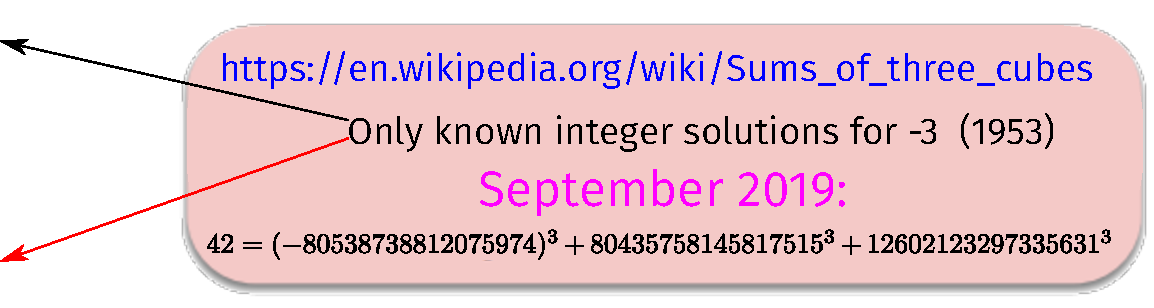
\includegraphics[scale=0.41]{nomajo1}}%
  \only<3>{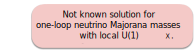
\includegraphics[scale=0.41]{nomajo}}%

  \qquad

  \vspace{2.8cm}
  \qquad
\end{column}
\end{columns}

\end{frame}


\begin{frame}
  \frametitle{Radiative Type-I seesaw \only<2>{with J. Calle and Ó. Zapata, arXiv:1909.09574}}
  \begin{columns}
    \begin{column}{0.65\textwidth}
      \def\rssc{0.26}
      \only<1>{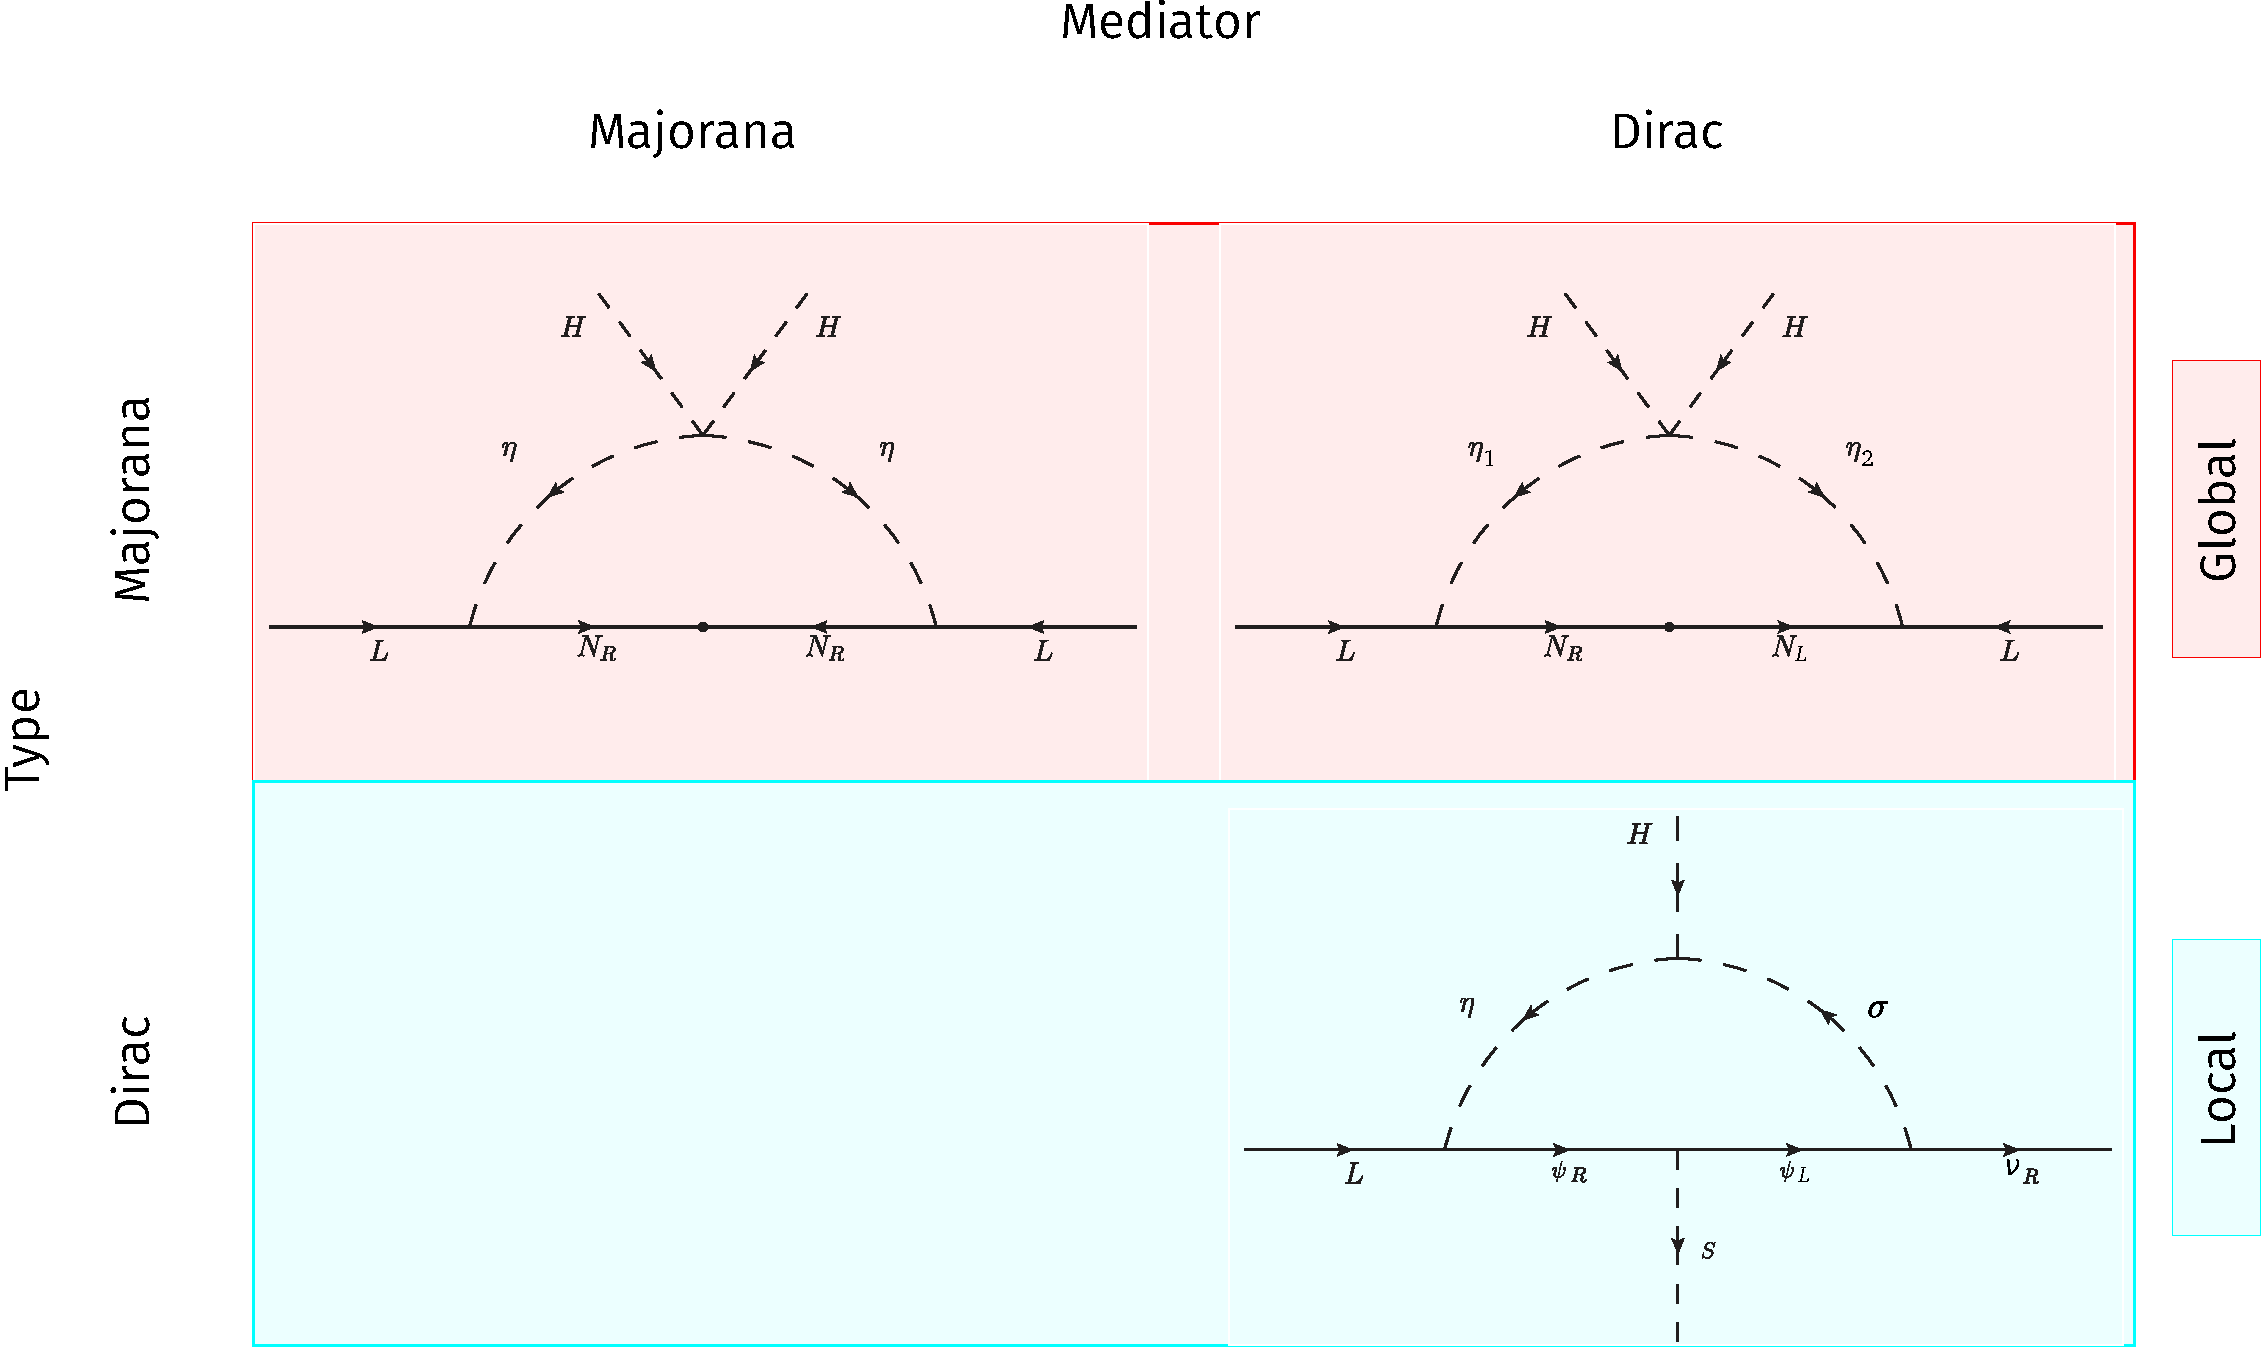
\includegraphics[scale=\rssc]{radiativeseesaw1}}%
      \only<2>{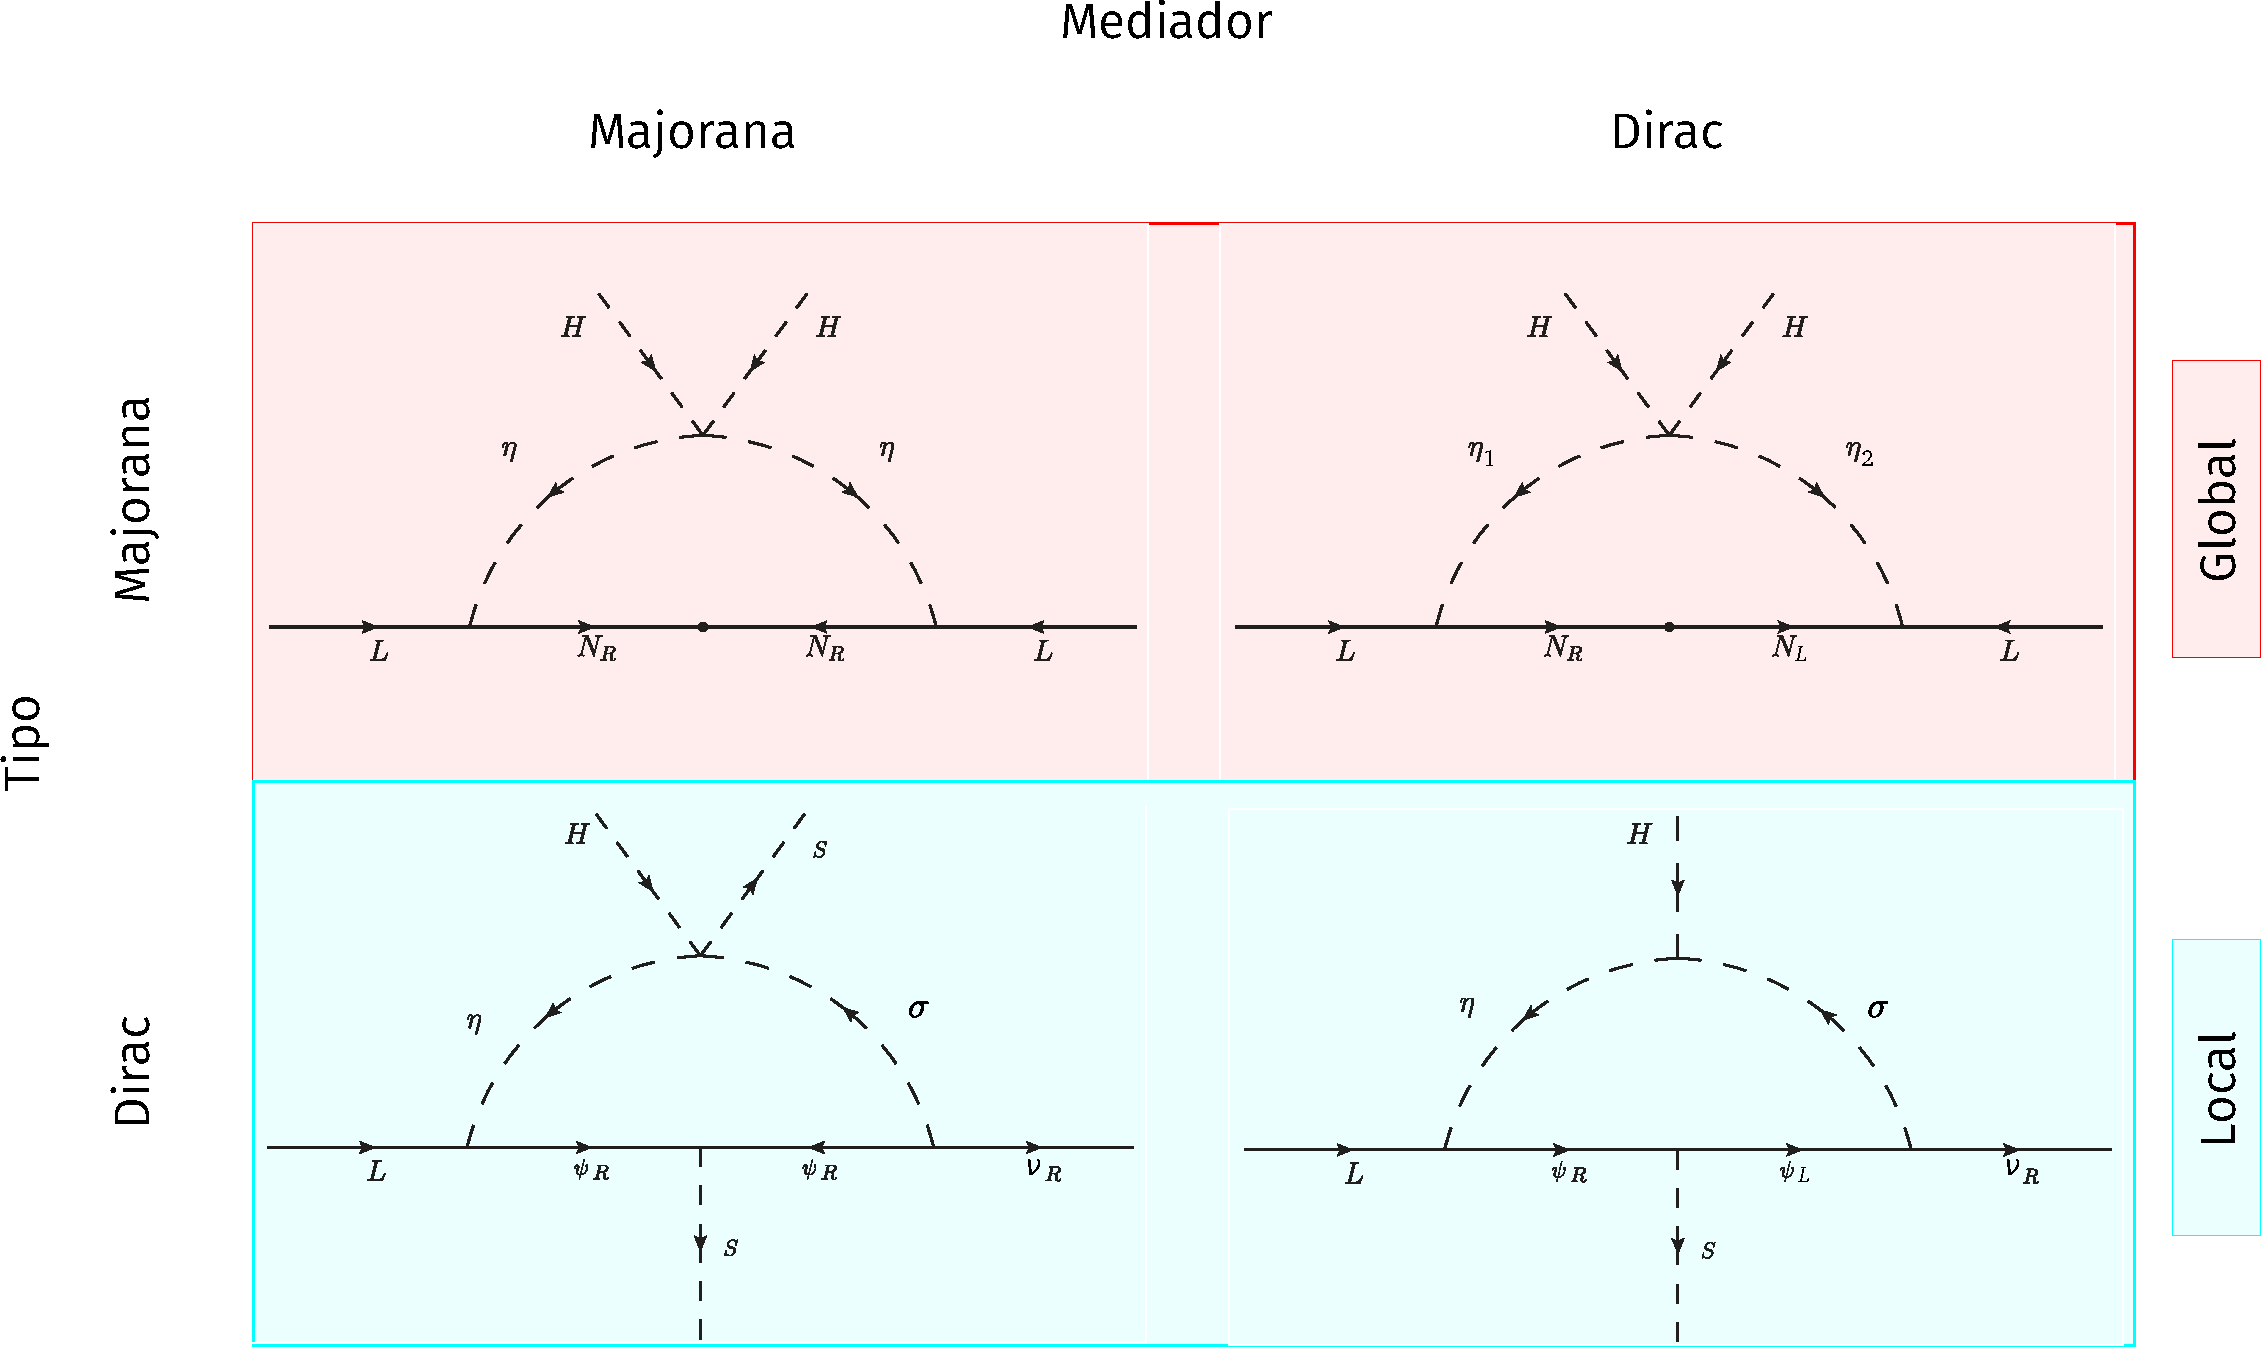
\includegraphics[scale=\rssc]{radiativeseesaw2}}%
      \only<3>{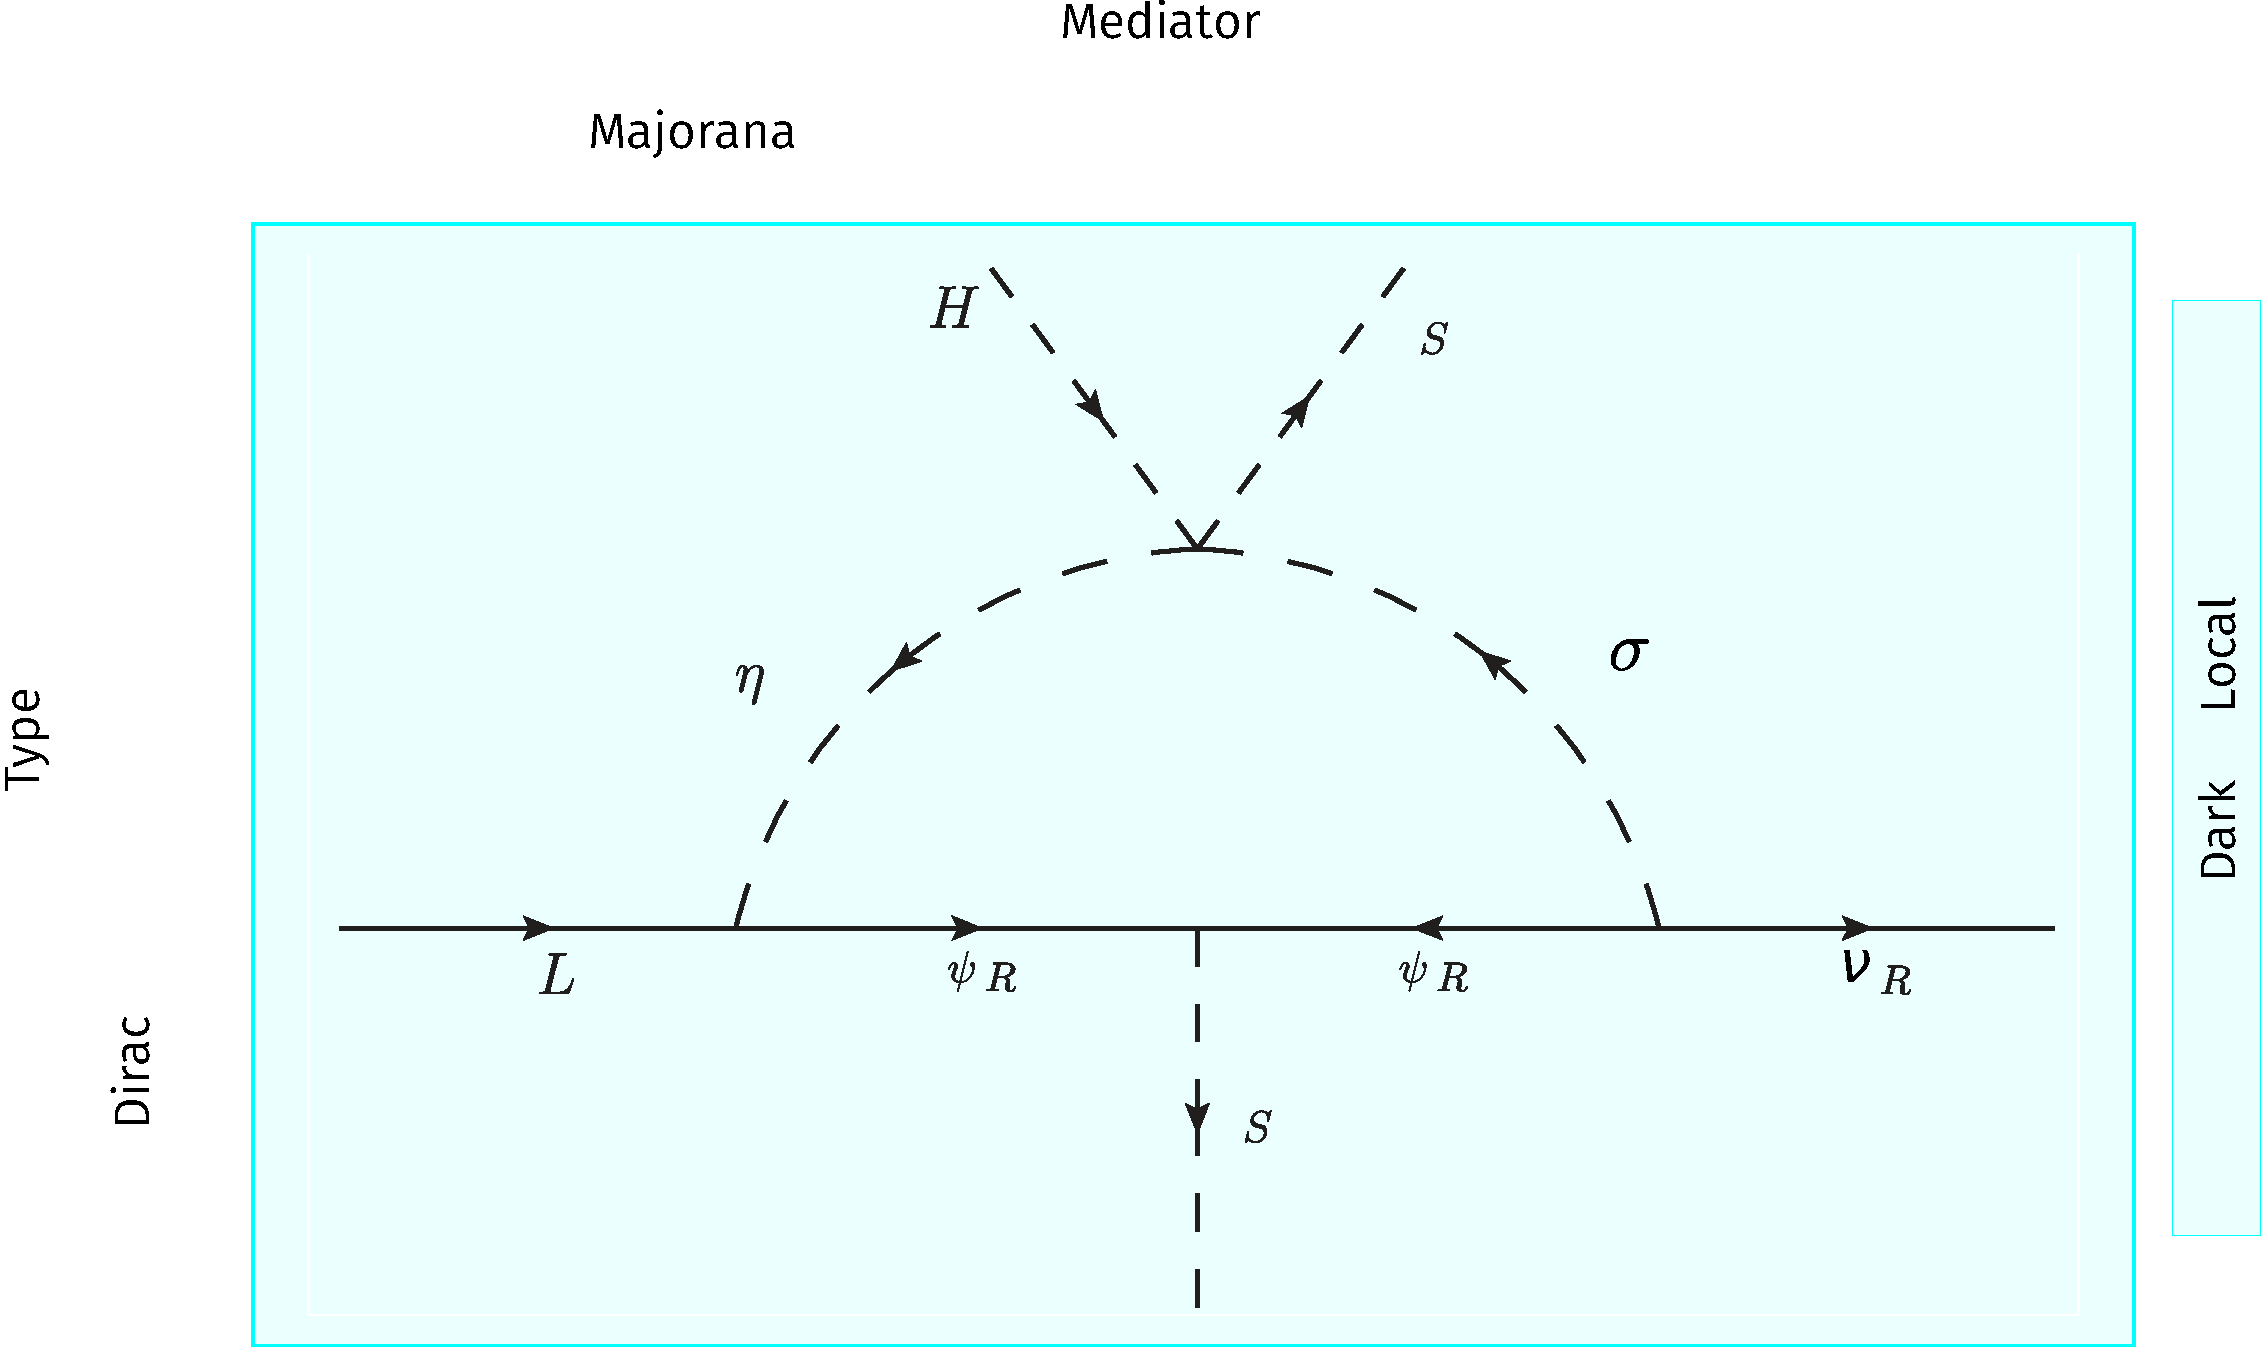
\includegraphics[scale=\rssc]{diracradiativeseesawmajo1}}%
      \only<4>{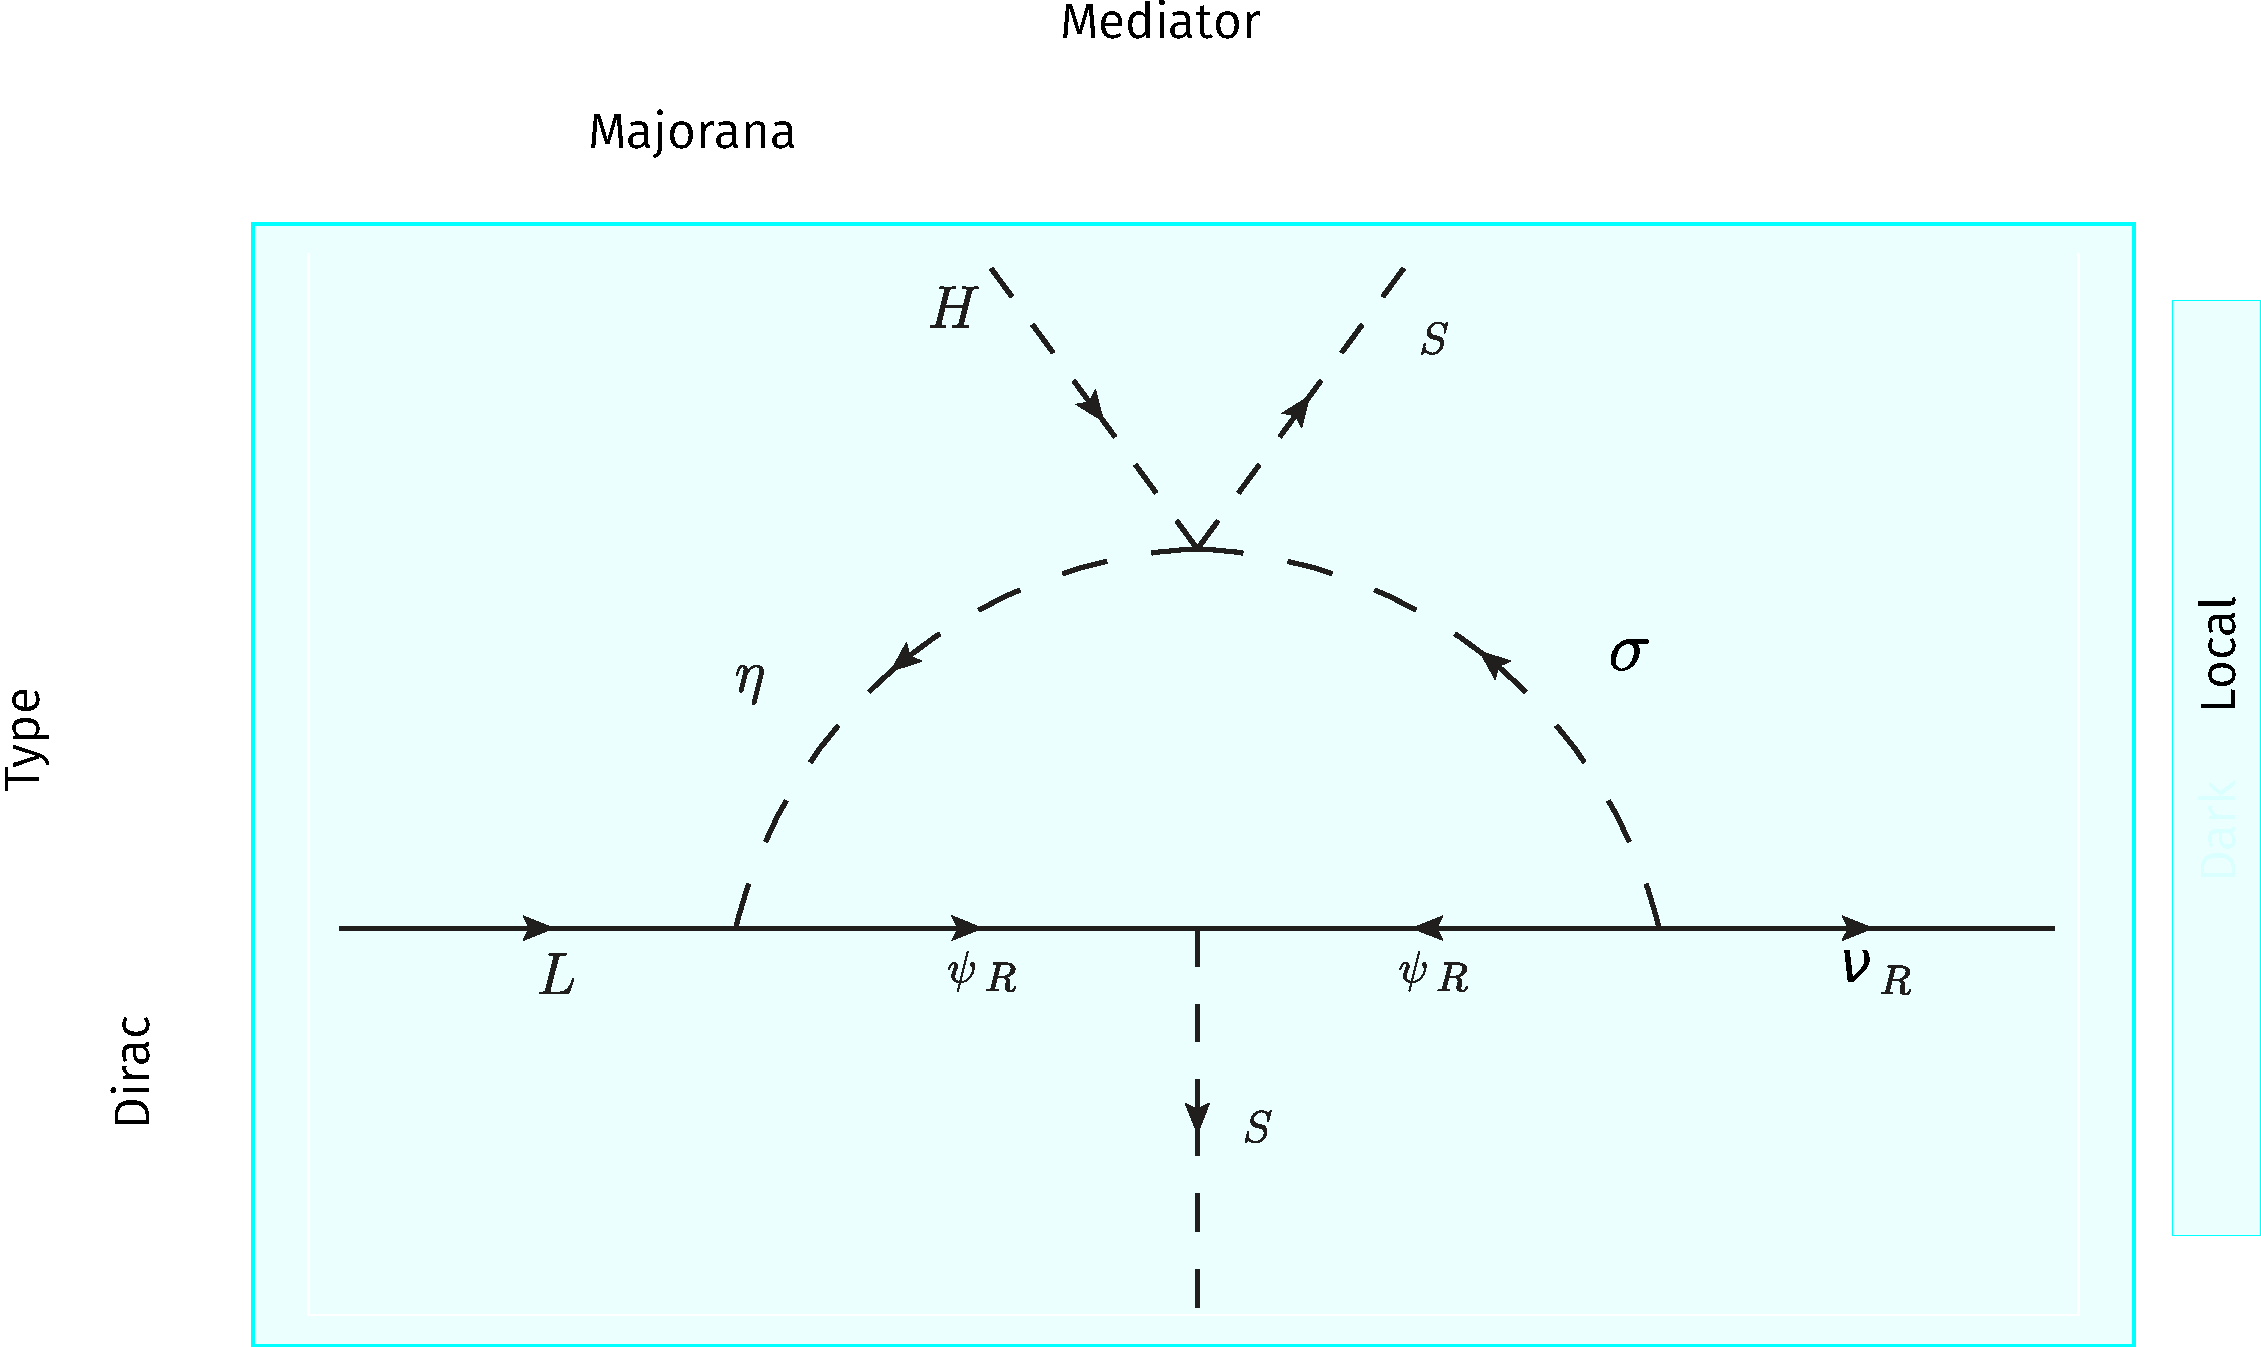
\includegraphics[scale=\rssc]{diracradiativeseesawmajo2}}%
      \only<5>{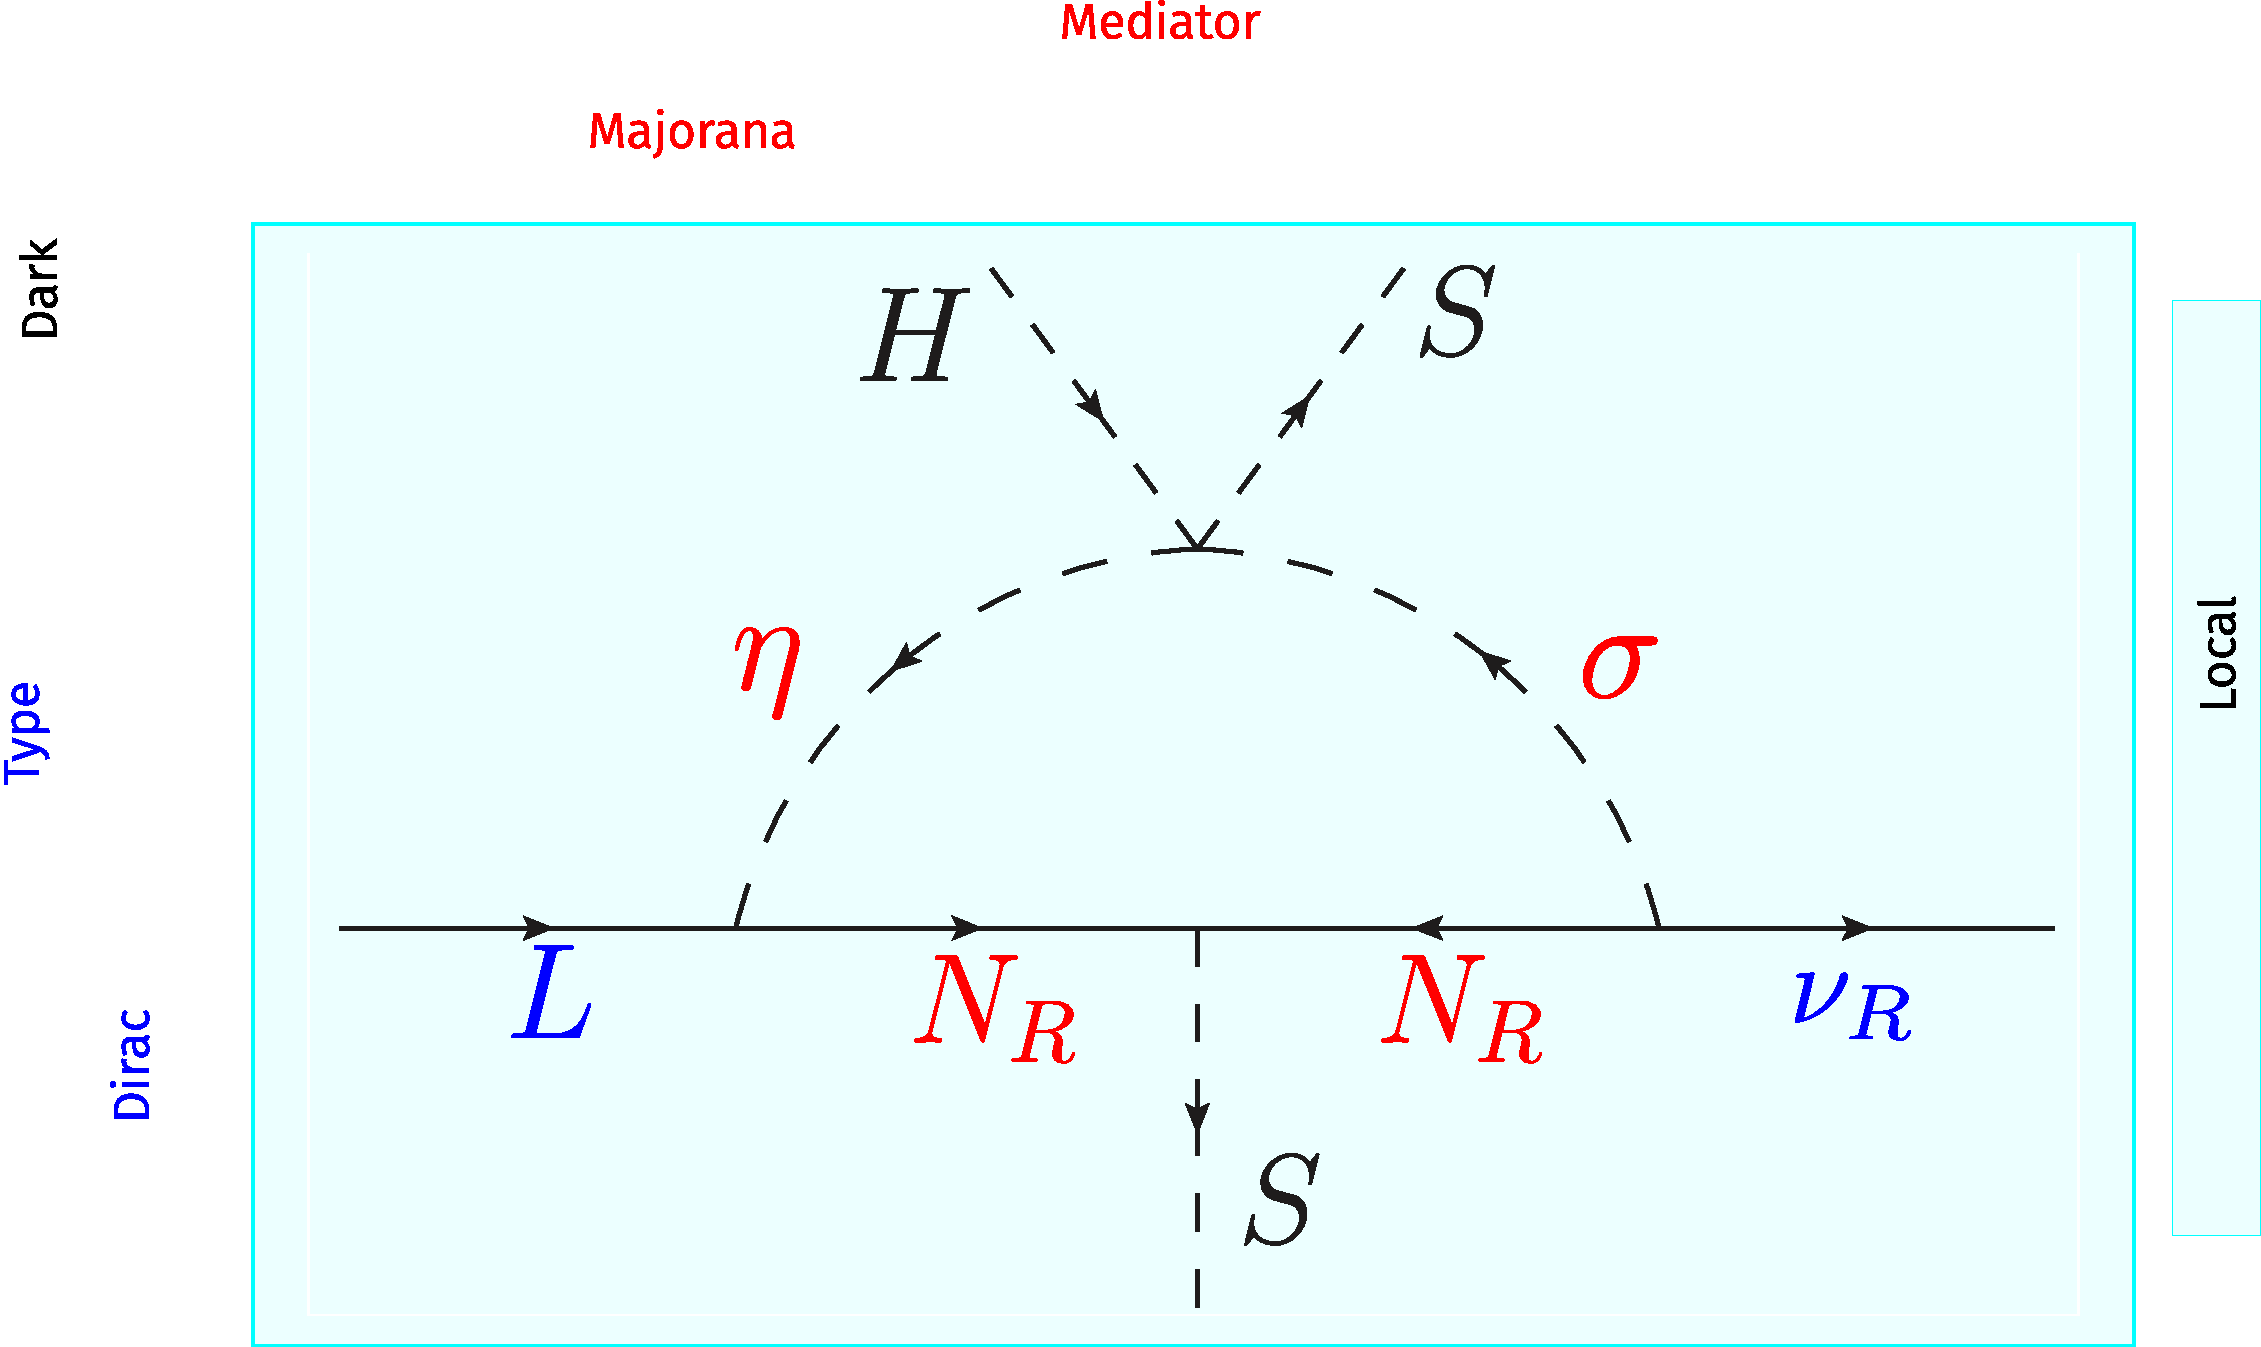
\includegraphics[scale=\rssc]{diracradiativeseesawmajo3}}%
      \only<6>{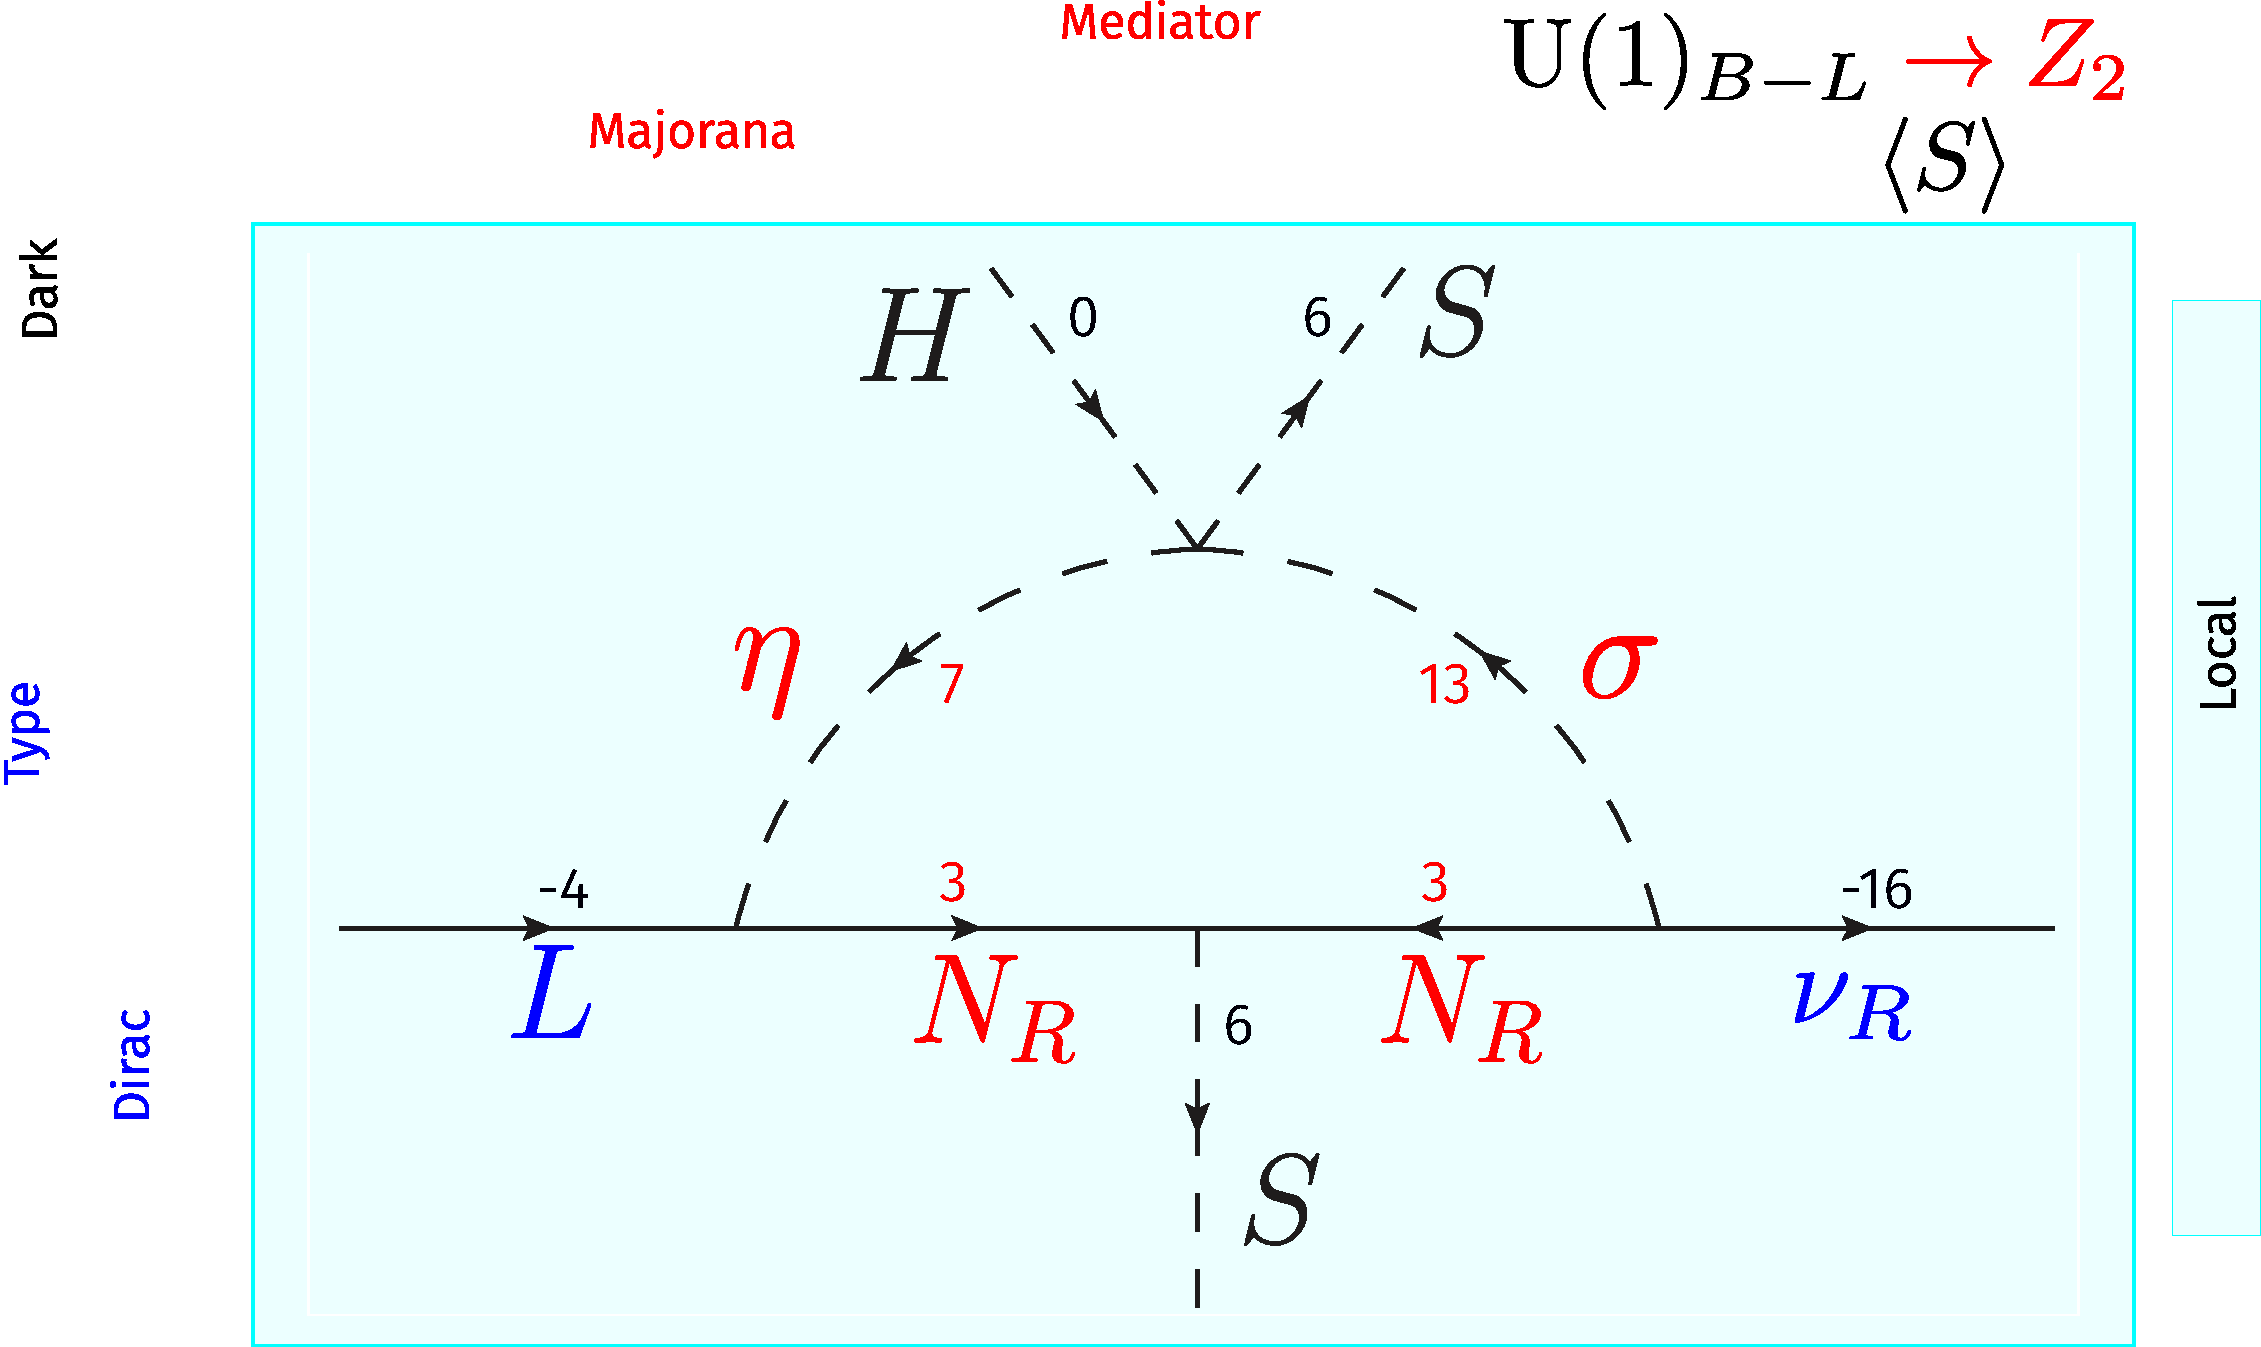
\includegraphics[scale=\rssc]{diracradiativeseesawmajo4}}%
      \invisible<1-2>{
        \begin{align*}
          N=&-\frac{\nu}{4}\invisible<1-4>{-\frac{1}{4}}\,,&\eta=&-\frac{\nu}{4}\invisible<1-4>{-\frac{1}{4}{\color{blue}\only<5>{-l}\only<6->{+1}}}\,,&\sigma=&-\frac{3\nu}{4}\invisible<1-4>{+\frac{1}{4}}\,.
\end{align*}
      }
    \end{column}
    \begin{column}{0.35\textwidth}
      \invisible<1-2>{
        \small
        \rowcolors{1}{RoyalBlue!20}{}
  \begin{tabular}{c|c|c|c}
    \hline  
    Fields   & $\operatorname{SU}(2)_L$ & $\operatorname{U}(1)_Y $  & $\operatorname{U}(1)_{  \only<3-4>{\mathcal{D}}\only<5>{X}\only<6->{B-L}   }$\\ \hline
$L $  & $\boldsymbol{2}$& $-1/2$&$\only<1-4>{0}\only<5>{{\color{blue}l}      }\only<6->{-1}$ \\    
$Q $  & $\boldsymbol{2}$& $-1/6$&$\only<1-4>{0}\only<5>{-{\color{blue}l}/3   }\only<6->{1/3}$ \\
$d_R $& $\boldsymbol{1}$& $-1/2$&$\only<1-4>{0}\only<5>{1+2{\color{blue}l}/3 }\only<6->{1/3}$ \\
$u_R $& $\boldsymbol{1}$& $+2/3$&$\only<1-4>{0}\only<5>{-1-4{\color{blue}l}/3}\only<6->{1/3}$ \\
$e_R $& $\boldsymbol{1}$& $-1$  &$\only<1-4>{0}\only<5>{1+2{\color{blue}l}   }\only<6->{-1}$ \\
$H $  & $\boldsymbol{2}$& $1/2$& $\only<1-4>{0}\only<5>{-1-{\color{blue}l}   }\only<6->{0}$\\\hline
$\eta$ & $\boldsymbol{2}$& $1/2$  &$\only<1-4>{1}\only<5>{3/4-\color{blue}l}  \only<6->{7/4}$ \\
$S$ & $\boldsymbol{1}$& $0$ &$\only<1-4>{2}\only<5->{3/2}$ \\    
$\sigma$ & $\boldsymbol{1}$& $0$ &$\only<1-4>{3}\only<5->{13/4}$ \\\hline        
    $\nu_{R1}$& $\boldsymbol{1}$& $0$ & ${-}4$\\
$\nu_{R2}$& $\boldsymbol{1}$& $0$ & ${-}4$\\
$\nu_{R3}$& $\boldsymbol{1}$& $0$ & $5$\\
$N_{R1}$& $\boldsymbol{1}$& $0$ & $\only<1-4>{1}\only<5->{3/4}$\\
$N_{R2}$& $\boldsymbol{1}$& $0$ & $\only<1-4>{1}\only<5->{3/4}$\\
$N_{R3}$& $\boldsymbol{1}$& $0$ & $\only<1-4>{1}\only<5->{3/4}$\\\hline\hline
\only<1-4>{TOTAL}\only<5->{$\xi_{L\alpha}$} &\only<5->{$\boldsymbol{1}$} &\only<5->{$0$}& $\only<1-4>{0}\only<5->{3/4}$ \\
  \end{tabular}
      }
    \end{column}
  \end{columns}
\end{frame}

\begin{frame}
  \frametitle{The model}
  
\begin{align*}
\label{eq:LagY}
    \mathcal{L} \supset& -\,g^{\prime}\,Z_\mu^\prime\sum_{F}q_{F}\overline{F} \gamma^\mu F+\sum_{\phi}\left|\left( \partial_\mu +i\,g^{\prime}\,q_\phi\,Z'_\mu \right) \phi\right|^2\nonumber\\
    &-[ 
    h_{i\alpha} \overline{L_{i}} \tilde{\eta} N_{R\alpha} +  y_{j\alpha} \overline{\nu_{R_{j}}} \sigma^* N^c_{R\alpha} + k_{\alpha} \overline{N^{c}_{R\alpha}} N_{R\alpha} S^* + \text{h.c.}] - \mathcal{V}(H, S, \eta, \sigma)\,.
\end{align*}
%
 $F$ ($\phi$) denote the new fermions (scalars)
\begin{align*}
%   \label{eq:VHSetasigma}
     \mathcal{V}(H, S, \eta, \sigma) = & V(H) + V(S) + V(\eta) + V(\sigma) \nonumber\\
     &+  \lambda_{HS} (H^{\dagger} H ) (S^{*} S) + \lambda_{2} (H^{\dagger} H ) (\sigma^{*} \sigma ) + \lambda_{3} (H^{\dagger} H ) (\eta^{\dagger} \eta )\nonumber\\
     &+ \lambda_{4} (S^{*} S) (\sigma^{*} \sigma ) + \lambda_{5} (S^{*} S) (\eta^{\dagger} \eta ) + \lambda_{6} (\eta^{\dagger} \eta ) (\sigma^{*} \sigma ) + \lambda_{7} (\eta^{\dagger} H ) (H^{\dagger} \eta ) \nonumber\\
     &+ \lambda_{8} (\eta^{\dagger} H S^{*} \sigma + \text{h.c.})\,,
\end{align*}

\end{frame}

\begin{frame}
  \frametitle{Neutrino masses and LFV}
\begin{align*}
(\mathcal{M}_{\nu})_{ij} = \frac{1}{32 \pi^{2}}  \frac{\lambda_8 v_S^2 v_H} {m_{\eta^0_R}^{2}-m_{\sigma^0_R}^{2}}\sum_{\alpha=1}^{3} h_{i \alpha} k_\alpha y^{*}_{j\alpha}\left[ F\left( \frac{m_{\eta^0_R}^{2}}{M_{N_{\alpha}}^{2}} \right) - F\left( \frac{m_{\sigma^0_R}^{2}}{M_{N_{\alpha}}^{2}} \right) \right] + (R \to I)\,,
\end{align*}
%
where $F(x) =x \log x/(x-1)$. 

\begin{block}{$\mu\to e \gamma$}
  \begin{columns}
    \begin{column}{0.5\textwidth}
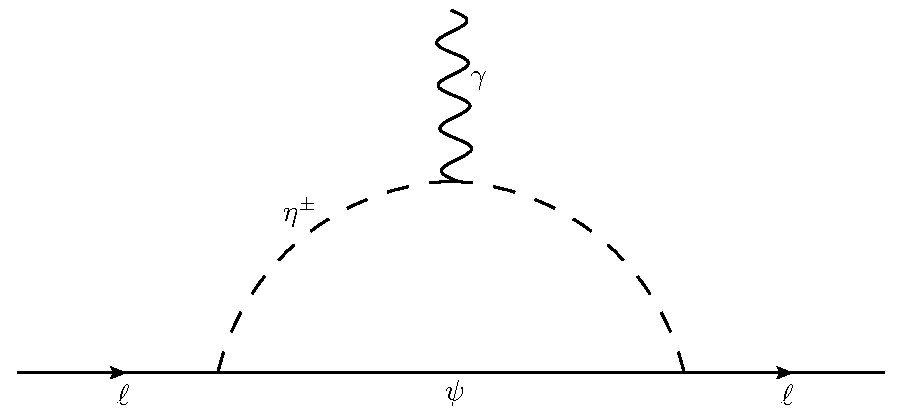
\includegraphics[scale=0.5]{LFV}           
    \end{column}
    \begin{column}{0.5\textwidth}
\begin{align*}
    \left| \sum_{\alpha}h_{2 \alpha} h_{1\alpha}^{*} \right| \lesssim 0.02 \left(\frac{m_\chi}{2\,\text{TeV}} \right)^{2}.
\end{align*}
    \end{column}
  \end{columns}
  

  


\end{block}

\end{frame}

\begin{frame}
\begin{picture}(320,250)
\only<1>{\put(-24,-30){\begin{overpic}[scale=0.352]{limits1}\end{overpic}}}%    
\only<2>{\put(-24,-30){\begin{overpic}[scale=0.352]{limits2}\end{overpic}}}%    
\only<3>{\put(-24,-30){\begin{overpic}[scale=0.352]{limits3}\end{overpic}}}%    
\only<4>{\put(-24,-30){\begin{overpic}[scale=0.352]{limits4}\end{overpic}}}%    
\only<5>{\put(-24,-30){\begin{overpic}[scale=0.352]{limits5}\end{overpic}}}%    
\only<6>{\put(-24,-30){\begin{overpic}[scale=0.352]{limits6}\end{overpic}}}%    
\end{picture}
\end{frame}

\section{(One-loop) Dirac neutrino masses}

%slide with sm dirac fermion explanation
\begin{frame}
  \frametitle{Lepton number}
  \begin{itemize}
  \item   Lepton number ($L$) is an accidental discret or Abelian symmetry of the standard model (SM). 
  \item  Without neutrino masses $L_e$, $L_{\mu}$, $L_{\tau}$ are also conserved.
  \item The processes which violates individual $L$ are called Lepton flavor violation (LFV) processes.
  \item All the neutrino mass models predict, to some extent, LFV processes
  \item Only models with Majorana neutrinos predict processes with total $L=L_e+L_{\mu}+L_{\tau}$ violation, like \alert{neutrino less doublet beta decay} (NLDBD).
  \item NLDBD is experimentally challenging, specially if there is a massless neutrino in the spectrum.
  \end{itemize}
\end{frame}


\begin{frame}
  \frametitle{NLDBD prospects for a  model with \alert{a massless
    neutrino} \tiny (arXiv:1806.09977 [PLB] with Reig, Valle and Zapata) }
     \begin{figure}
      \centering
      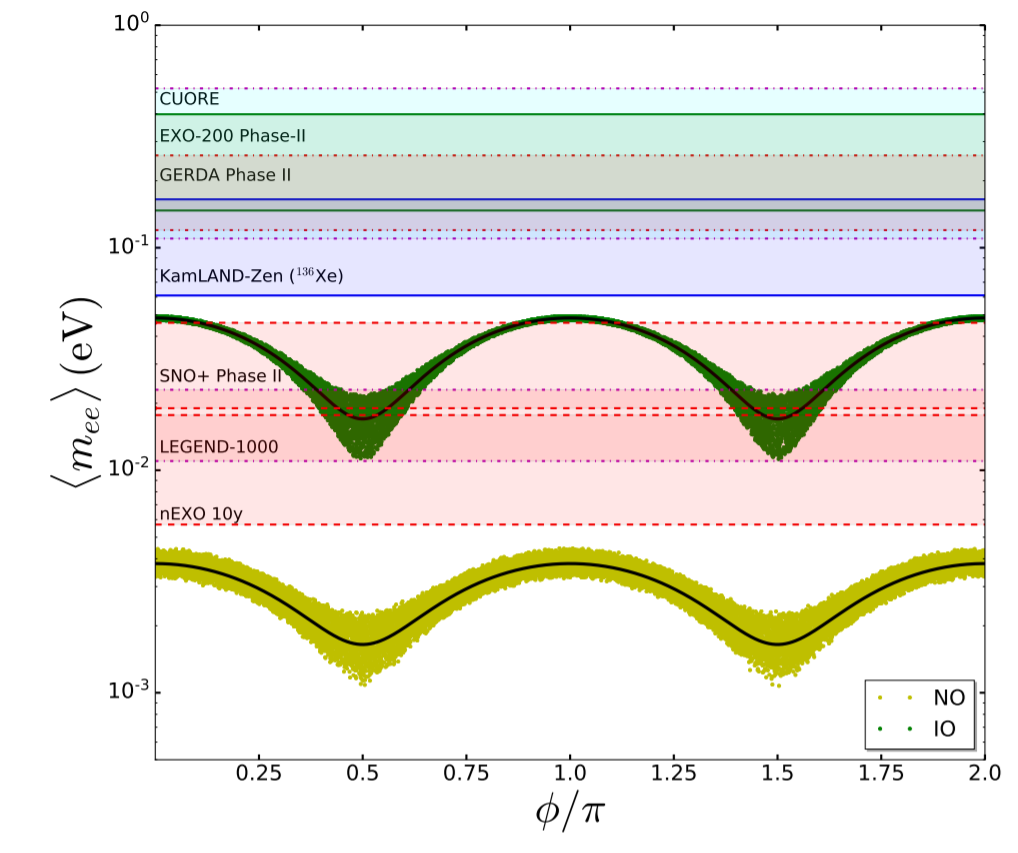
\includegraphics[scale=0.25]{mee}\\
      {\tiny  with M.Reig, J.W.F Valle, O. Zapata, arXiv:1806.09977  }
    \end{figure}

 
\end{frame}


\begin{frame}
  \frametitle{Total lepton number: $L=L_e+L_{\mu}+L_{\tau}$}
  \begin{columns}
    \begin{column}{0.48\textwidth}
      \begin{block}{\centering Majorana $\cancel{\operatorname{U}(1)_L}$}
              \centering
    \rowcolors{1}{RoyalBlue!20}{}
\begin{tabular}{cc}
  Field &  $Z_2\ (\omega^2=1)$ \\\hline
  SM & $1$\\
  $L$& $\omega$ \\
     $ \left( e_R \right)^{\dagger}  $& $\omega$ \\
    $\left( \nu_R \right)^{\dagger}$ & $\omega$ \\\hline
    \end{tabular}

    \begin{align*}
      \mathcal{L}_{\nu}=h_D \left( \nu_R \right)^{\dagger}L \cdot H +
{\color{red}M_R\,\nu_R \nu_R}
      +\text{h.c}\,.
    \end{align*}
    \begin{align*}
      h_D \sim  \mathcal{O}(1) 
    \end{align*}
    \invisible<1->{Explain smallness ala Peccei-Quinn:
    \vspace{-0.5cm}
    \begin{align*}
      \operatorname{U}(1)_{B-L}\to Z_N\,,\quad N\ge 3\,.
    \end{align*}}    

      \end{block}
    \end{column}
  \begin{column}{0.48\textwidth}
    \begin{block}{\centering Dirac $\only<1>{\operatorname{U}(1)_L}
        \only<2>{\operatorname{U}(1)_{B-L}}$}
              \centering
    \rowcolors{1}{RoyalBlue!20}{}
\begin{tabular}{cc}
  Field &  $Z_3\ (\omega^3=1)$ \\\hline
  SM & $1$\\
  $L$& $\omega$ \\
       $ \left( e_R \right)^{\dagger}  $& $\omega^2$ \\
    $\left( \nu_R \right)^{\dagger}$ & $\omega^2$ \\\hline
    \end{tabular}

    \begin{align*}
      \mathcal{L}_{\nu}=h_D \left( \nu_R \right)^{\dagger}L \cdot H 
      +\text{h.c}\,.
    \end{align*}
    \begin{align*}
      h_D \sim \mathcal{O}(10^{-11}) 
    \end{align*}
    \invisible<1>{Explain smallness ala Peccei-Quinn:
      \vspace{-0.5cm}
    \begin{align*}
      \operatorname{U}(1)_{B-L} \underbrace{\longrightarrow}_{\color{red}\left\langle S \right\rangle} Z_N\,,\quad N\ge 3\,.
    \end{align*}}    
      \end{block}
    
  \end{column}
\end{columns}

\end{frame}



\begin{frame} 
  \frametitle{Small Dirac neutrino masses}
  \begin{columns}
    \begin{column}{0.78\textwidth}
      \small \qquad
      
      \vspace{0.2cm}
      
  To explain the \alert{smallness} of Dirac neutrino masses choose $\operatorname{U}(1)_{B-L} $ which:
  \begin{itemize}
  \item<1-> Forbids tree-level mass (TL) term ( $Y(H)=+1/2$ )
    \begin{align*}
      \mathcal{L}_{\text{T.L}}=&h_{D}\epsilon_{ab} \left( \nu_R \right)^{\dagger} L^a H^b +\text{h.c}\\
      =&h_D\left( \nu_R \right)^{\dagger} L\cdot  H +\text{h.c}\\
    \end{align*}
    \vspace{-1.5cm}
  \item<2-> Forbids Majorana term: $\nu_R \nu_R$
        \vspace{-0.3cm}
   \item<3-> Realizes of the 5-dimension operator which conserves lepton number in    $\operatorname{SU}(3)_c \times\operatorname{SU}(2)_L\times \operatorname{U}(1)_Y\times \operatorname{U}(1)_{B-L}$:
     \begin{align*}
       \mathcal{L}_{5-D}= \frac{h_\nu }{\Lambda}\left( \nu_R \right)^{\dagger} L\cdot H
       {\color{red}S}+\text{h.c}\\
     \end{align*}
             \vspace{-0.3cm}
           \item<4-> Enhancement to the \emph{effective number of degrees of freedom in the early Universe} $\Delta N_{\text{eff}}=N_{\text{eff}}-N_{\text{eff}}^{\text{SM}}$ ({\tiny see arXiv:1211.0186})             
  \end{itemize}

  \invisible<1-3>{See E. Ma, Rahul Srivastava: arXiv:1411.5042 [PLB] for tree-level realization} 
    \end{column}
    \begin{column}{0.22\textwidth}
      \invisible<1-2>{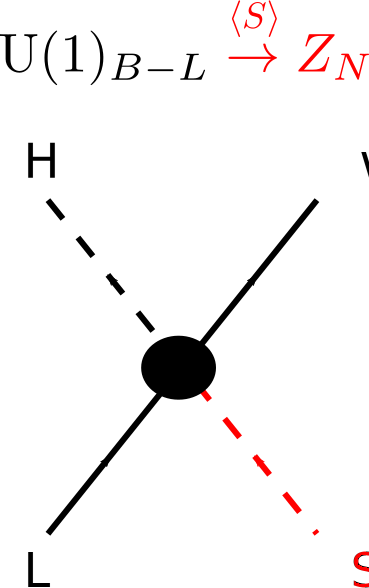
\includegraphics[scale=0.2]{l5d}}
    \end{column}
  \end{columns}

\end{frame}

\begin{frame}
  \frametitle{From {1210.6350} and
    {1805.02025}: $\Delta N_{\text{eff}}=3 \left( T_{\nu_R}/T_{\nu_L} \right)^4$    }
  \begin{columns}
    \begin{column}{0.5\textwidth}
      \footnotesize
      \begin{align*}
{\color{blue} \Gamma_{\nu_R}(T)}&=n_{\nu_R}(T)\sum_f \langle \sigma_f(\nu_R \bar{\nu}_R\to f\bar{f})v \rangle \\ 
&= \sum_f \frac{g_{\nu_R}^2}{n_{\nu_R}}\int \frac{d^3 p }{(2\pi)^3} \frac{d^3 q }{(2\pi)^3}
f_{\nu_R}(p)f_{\nu_R}(q) \sigma_f(s) (1-\cos\theta),
      \end{align*}
\vspace{-0.5cm}      
      \begin{align*}
        s=&2pq(1-\cos\theta),& f_{\nu_R}(k)=& 1/(e^{k/T}+1)\\
        n_{\nu_R}(T)=&g_{\nu_R}\int \frac{d^3k}{(2\pi)^3}f_{\nu_R}(k),& \text{with } g_{\nu_R}=&2\\
        \sigma_f(s)\simeq&\frac{ N_C^f ( { \only<1>{\color{black}}\only<2>{\color{red}}  Q_{BL}^f}   )^2 Q^2 s}{12\pi}\left(\frac{g'}{M_{Z'}}\right)^4,&
       \text{In the limit } M^2_{Z'}\gg& s\,.
      \end{align*}
with three right-handed neutrinos, the Hubble parameter is 
\begin{equation*}
  {\color{blue}H(T)}=\sqrt{\frac{4\pi^3G_N \left[ {  \only<1>{\color{red}}\only<2>{\color{black}}  g(T)}+{21}/{4} \right]}{45}}\,T^2.
\end{equation*}

The right-handed neutrinos decouple when
\begin{align*}
  \color{blue}
  \Gamma_{\nu_R}(T^{\nu_R}_\text{dec})=H(T^{\nu_R}_\text{dec}).
\end{align*}

    \end{column}
    \begin{column}{0.5\textwidth}
      \centering
      \invisible<1>{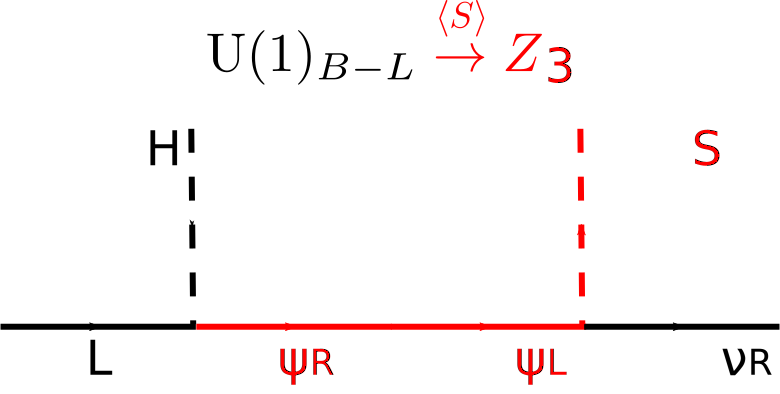
\includegraphics[scale=0.14]{tree-level-dirac-seesaw}

      {\scriptsize
          \rowcolors{1}{RoyalBlue!20}{}
  \begin{tabular}{cccccc}\hline
   $ \nu_{R3} $
  &$\nu_{R2} $&$\nu_{R1}$&$\psi_L$&$ \psi_R  $&$S$\\ \hline
  $\color{red}-4$&$\color{red}-4$&$\color{red}+5$& $\color{black}-1$ & $\color{black}-1$ & $+3$\\\hline
  \end{tabular}

  {\tiny E. Ma, R. Srivastava: arXiv:1411.5042 [PLB]}
}}
\def\scf{4.9cm}
\only<1>{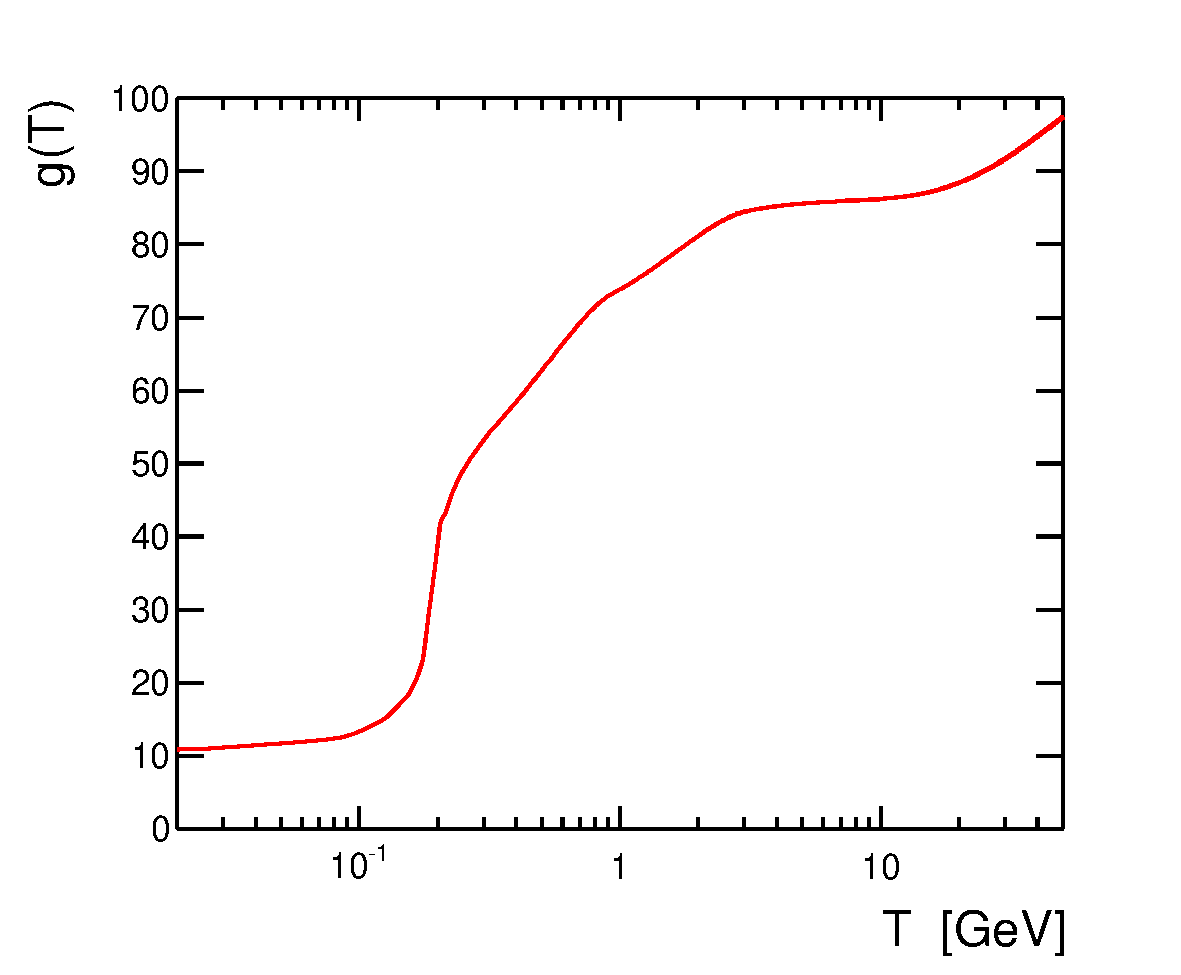
\includegraphics[height=4.5cm]{gT}

  {\tiny A. Solaguren-Beascoa, M. C. Gonzalez-Garcia: arXiv:{\color{red}1210.6350} [PLB]

\qquad
  }
}%
\only<2->{%
\only<2>{ 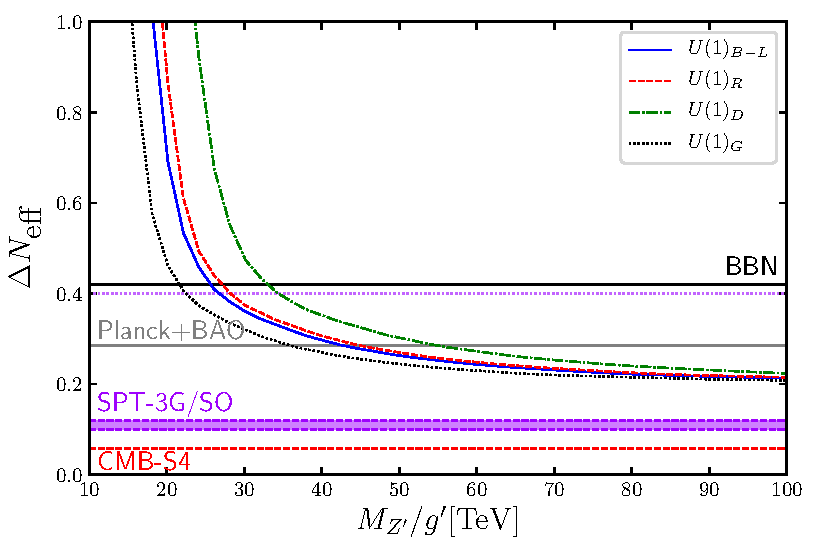
\includegraphics[height=\scf]{D_Neff}}%
\only<3->{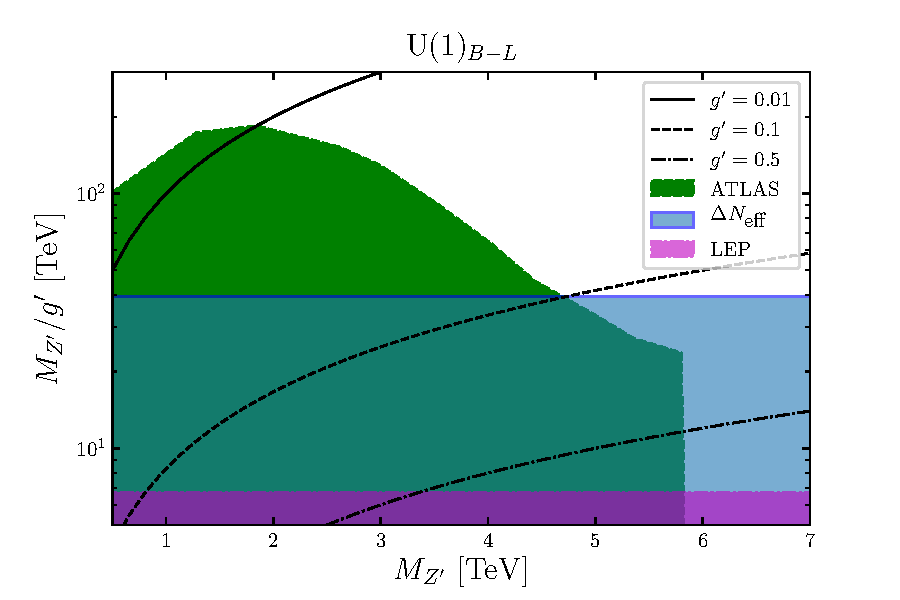
\includegraphics[height=\scf]{u1blc}}

  {\tiny with J. Calle and Ó. Zapata, arXiv:1909.09574

%    (also: Planck 1807.06209, Riess \emph{et al} 1903.07603 )
  }
}
    \end{column}
  \end{columns}
\end{frame}

%\section{Dark symmetry}



\begin{frame}
  \frametitle{Same constraints as before}
  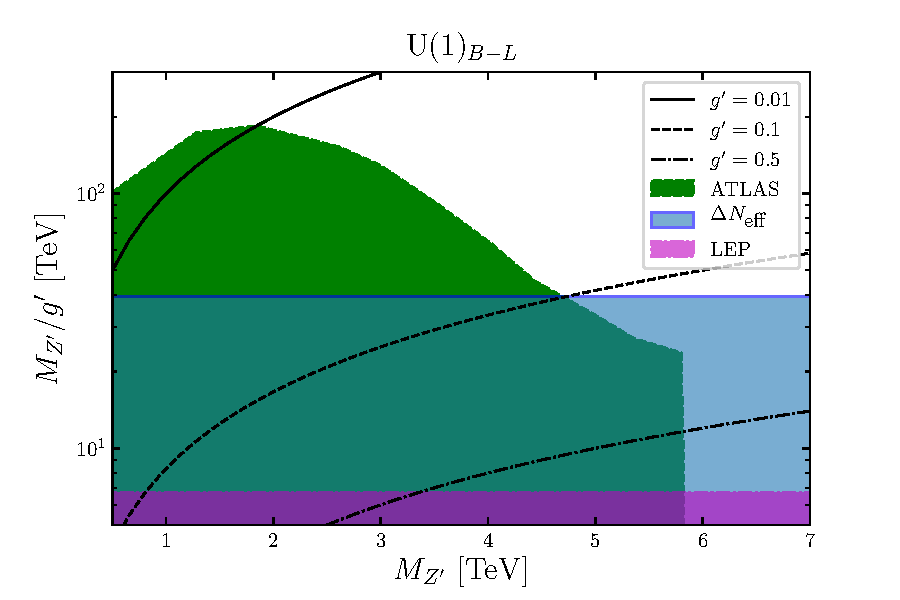
\includegraphics[height=8cm]{u1blc}

  {\tiny with J. Calle and Ó. Zapata, arXiv:1909.09574
  }
\end{frame}

\begin{frame}
\frametitle{Conclusions}
  It makes sense to focus our attention on models tha can account for neutrino masses and dark matter (DM) \alert{without adhoc symmetries}
\only<1>{
  \begin{block}{One-loop Dirac neutrino masses}
      A single $U(1)_X$ gauge symmetry to explain both the smallnes of Dirac neutrino masses and the stability of Dirac fermion dark matter
  %\setbeamercolor{block body}{use=structure,fg=black,bg=white}
    \begin{itemize}
    \item Spontaneously broken $U(1)_{X}$ generates a radiative Dirac neutrino masses
  \item A remnant symmetry makes the lightest field circulating the loop stable and good dark matter candidate.
  \item For T1-2-A: Either Singet Doublet Dirac Dark Matter or Singlet Scalar Dark Matter with extra scalar and vector portal
  \item Dark symmetry for Majorana mediatiors
    \end{itemize}
  \end{block}
}

\end{frame}




\section{One-loop realization of $\mathcal{L}_{5-D}$ with total $L$}
\begin{frame}
\begin{picture}(320,250)
\only<1>{\put(-24,-21){\begin{overpic}[scale=0.352]{u11}\end{overpic}}}%
\only<2>{\put(-24,-21){\begin{overpic}[scale=0.352]{u12}\end{overpic}}}%
\only<3>{\put(-24,-21){\begin{overpic}[scale=0.352]{u13}\end{overpic}}}%
\only<4>{\put(-24,-21){\begin{overpic}[scale=0.352]{u14}\end{overpic}}}%
\end{picture}
\end{frame}

\begin{frame}
  \frametitle{\only<1>{One-loop topologies $\operatorname{U}(1)_{B-L}\oplus Z_2 \oplus Z_2 $}\only<2-4>{One-loop topologies $\operatorname{U}(1)_{B-L}$ only!
   \invisible<2>{\scriptsize with J. Calle, C. Yaguna, and O. Zapata, arXiv:1812.05523 [PRD]  } }\only<5-6>{
    SD${}^{3}$M+SSDM: $\sigma_a$ ($a=1,2$)     \invisible<6>{\scriptsize with J. Calle, C. Yaguna, and O. Zapata, arXiv:1812.05523 [PRD]  }  }}
\begin{picture}(320,250)
  \only<1>{\put(40,20){\begin{overpic}[scale=0.6]{radiativedirac1}\end{overpic}}}%
  \only<1>{\put(280,130){\tiny Chang-Yuan Yao and Gui-Jun Ding, arXiv:1802.05231 [PRD]  }}%
  \only<2>{\put(40,20){\begin{overpic}[scale=0.6]{radiativedirac2}\end{overpic}}}%
  \only<2>{\put(280,130){\tiny with J. Calle, C. Yaguna, and O. Zapata, arXiv:1812.05523 [PRD]  }}%
    \only<2-5>{\put(-20,130){\tiny
        \begin{minipage}{0.3\linewidth}
          \begin{align*}
            \psi_{L,R}\to&\text{Singlet fermions \only<3>{(vector-like)}\only<4-5>{(quiral)}  }\\
            \invisible<3>{\Psi_{L,R}\to&\text{Vector-like doublet fermions}\invisible<2-4>{:\qquad {\color{red}10/5}}   }\\
            \sigma\to&\text{Singlet scalar}\invisible<2-4>{:\qquad 15/5}   \\
            \invisible<5>{\eta\to&\text{Doublet scalar}   }
          \end{align*}
        \end{minipage}
}}%
\only<3>{\put(40,20){\begin{overpic}[scale=0.6]{radiativedirac3}\end{overpic}}}%
% 
\only<3>{\put(160,230){\tiny $\longmapsto$ ${\color{Green}\sigma_1}={\color{red}-2}$\,,\qquad
                             ${\color{red}\sigma_2}={\color{Yellow}-5}$\,,\qquad }}%
\only<3>{\put(160,220){\tiny $\longmapsto$ generalization to two and three loops: S. Saad arXiv:1902.07259 [NPB]  }}%
\only<3>{\put(160,210){\tiny $\longmapsto$ generalization to $\operatorname{U(1)_R}$: \emph{et al}, S. Saad arXiv:1904.07407  }}%
\only<3>{\put(180,180){\Huge $\uparrow$   }}%
\only<3-5>{\put(240,135){\tiny
    \begin{minipage}{0.3\linewidth}
      \rowcolors{1}{RoyalBlue!20}{}
  \begin{tabular}{c|cccccc}\hline
 Fields: $f_i$  &  $\left( \nu_{R3} \right)^{\dagger}$
  &$\left( \nu_{R2} \right)^{\dagger}$&$\left( \nu_{R1} \right)^{\dagger}$&$\psi_L$&$\left( \psi_R \right)^{\dagger}$&$S$\\ \hline
  (A)&$\color{Yellow}+4$&$\color{Yellow}+4$&$-5$& $\color{red}-r$ & $\color{red}r$ & $+3$\\
    \invisible<3>{(B) &$\displaystyle{+\frac{8}{5}}$&$\displaystyle{+\frac{8}{5}}$&$\displaystyle{+\frac{2}{5}}$&$\displaystyle{\frac{7}{5}}$&$\color{red}\displaystyle{-\frac{10}{5}}$&$\color{blue}\displaystyle{+\frac{3}{5}}$}\\
  \end{tabular}
         \end{minipage}
       }}%
\only<3-5>{\put(300,55){\tiny
    \begin{minipage}{0.3\linewidth}
       \begin{center}
         \textbf{Anomaly cancellation conditions}
         \begin{align*}
           \sum_i f_i=& 3 \\
           \sum_i f_i^3=& 3 \\
         \end{align*}
  \end{center}
      
         \end{minipage}
       }}%
%  effective number of relativistic degrees of reedom Neff for neutrinos
 \only<4>{\put(40,20){\begin{overpic}[scale=0.6]{radiativedirac4}\end{overpic}}}%
 \only<5-6>{\put(40,20){\begin{overpic}[scale=0.6]{radiativedirac5}\end{overpic}}}%
 \only<6>{\put(20,200){
     \begin{minipage}{0.3\linewidth}
       $M_\psi=h_1 \left\langle S \right\rangle$, $\color{red}y_2=0$:
          \begin{align*}
            \mathcal{L}={\color{red}\mathcal{L}_{\text{SD${}^3$M}}}
            +{\color{Green} h_3^{ia} \widetilde{\left( \Psi_R \right)}\cdot L_i\, \sigma_a}+
      {\color{blue}      h_2^{\beta a} \left( \nu_{R\beta} \right)^{\dagger} \psi_L\, \sigma^{*}_a}
            -V(\sigma_a,S,H)\,.
          \end{align*}
        \end{minipage}
}}%
\only<6>{\put(0,130){\small with A.F Rivera, W. Tangarife,  arXiv:1906.09685 [PRD]   }}%
\only<6>{\put(220,60){\begin{overpic}[scale=0.6]{sarah}\end{overpic}}}%
\end{picture}
\end{frame}

\section{Singlet-Doublet Dirac Dark matter Model (SD${}^{3}$M)}
\begin{frame}
  \frametitle{ Singlet-Doublet Dirac Dark Matter (SD${}^{3}$M)
By Carlos E. Yaguna.
arXiv:1510.06151 [PRD].
}

The model extends the standard model (SM) particle content with Dirac Fermions: from  $\operatorname{SU}(2)$ doublets of Weyl fermions: $\Psi_L=\left( \Psi_L^0,\, \Psi_L^-\right)^{\operatorname{T}}$, $\widetilde{\left( \Psi_R \right)}=\left( (\Psi_R^-)^\dagger,\, -(\Psi_R^0)^\dagger\right)^{\operatorname{T}}$  and singlet Weyl fermions $\psi_{LR}$ that interact among themselves and with the SM fields 
\begin{align}
  \mathcal{L}\supset& {\color{red} M_{\psi}}\left( \psi_R \right)^{\dagger}\psi_L
%+ {\color{red}h_S} \left( \psi_R \right)^{\dagger} \psi_LS  %+\text{h.c}.
%  \mathcal{L}_{\psi}+\mathcal{L}_{\sigma\psi}
+ %\left[
{\color{red}M_{\Psi}}\widetilde{\left( \Psi_R \right)}\cdot  \Psi_L
% +h_2^{ia} \widetilde{\left( \Psi_R \right)}\cdot L_i\, \sigma_a
+ {\color{red} y_1} \left( \psi_R \right)^{\dagger} \Psi_L \cdot H
+ {\color{red} y_2}  \widetilde{\left( \Psi_R \right)} \cdot \widetilde{H} \psi_L
                      +\text{h.c} % \right]
%+V(\sigma_a,S,H)\,,
\end{align}
Four free parameters:
\begin{align}
  {\color{red} M_{\psi}},{\color{red}M_{\Psi}}\ <& 2\text{ GeV}\,,&
  {\color{red} y_1},\ {\color{red} y_2} > 10^{-6}
\end{align}
Two neutral Dirac fermion eigenstates:
\begin{align}
  M=&
  \begin{pmatrix}
    {\color{red}M_{\psi}} & {\color{red}y_{2}} v/\sqrt{2} \\ {\color{red}y_{1}} v/\sqrt{2} & {\color{red} M_{D}}
  \end{pmatrix},&
M_{\text{diag}}=&
\begin{pmatrix}
{M_{\chi_{1}}} & {0} \\ {0} & {M_{\chi_{2}}}                    
\end{pmatrix}
=U_{L}^{\dagger} M U_{R}
\end{align}


\end{frame}


\begin{frame}
    \frametitle{ SD${}^{3}$M
By Carlos E. Yaguna.
arXiv:1510.06151 [PRD].
}
    \begin{columns}
    \begin{column}{0.5\textwidth}
      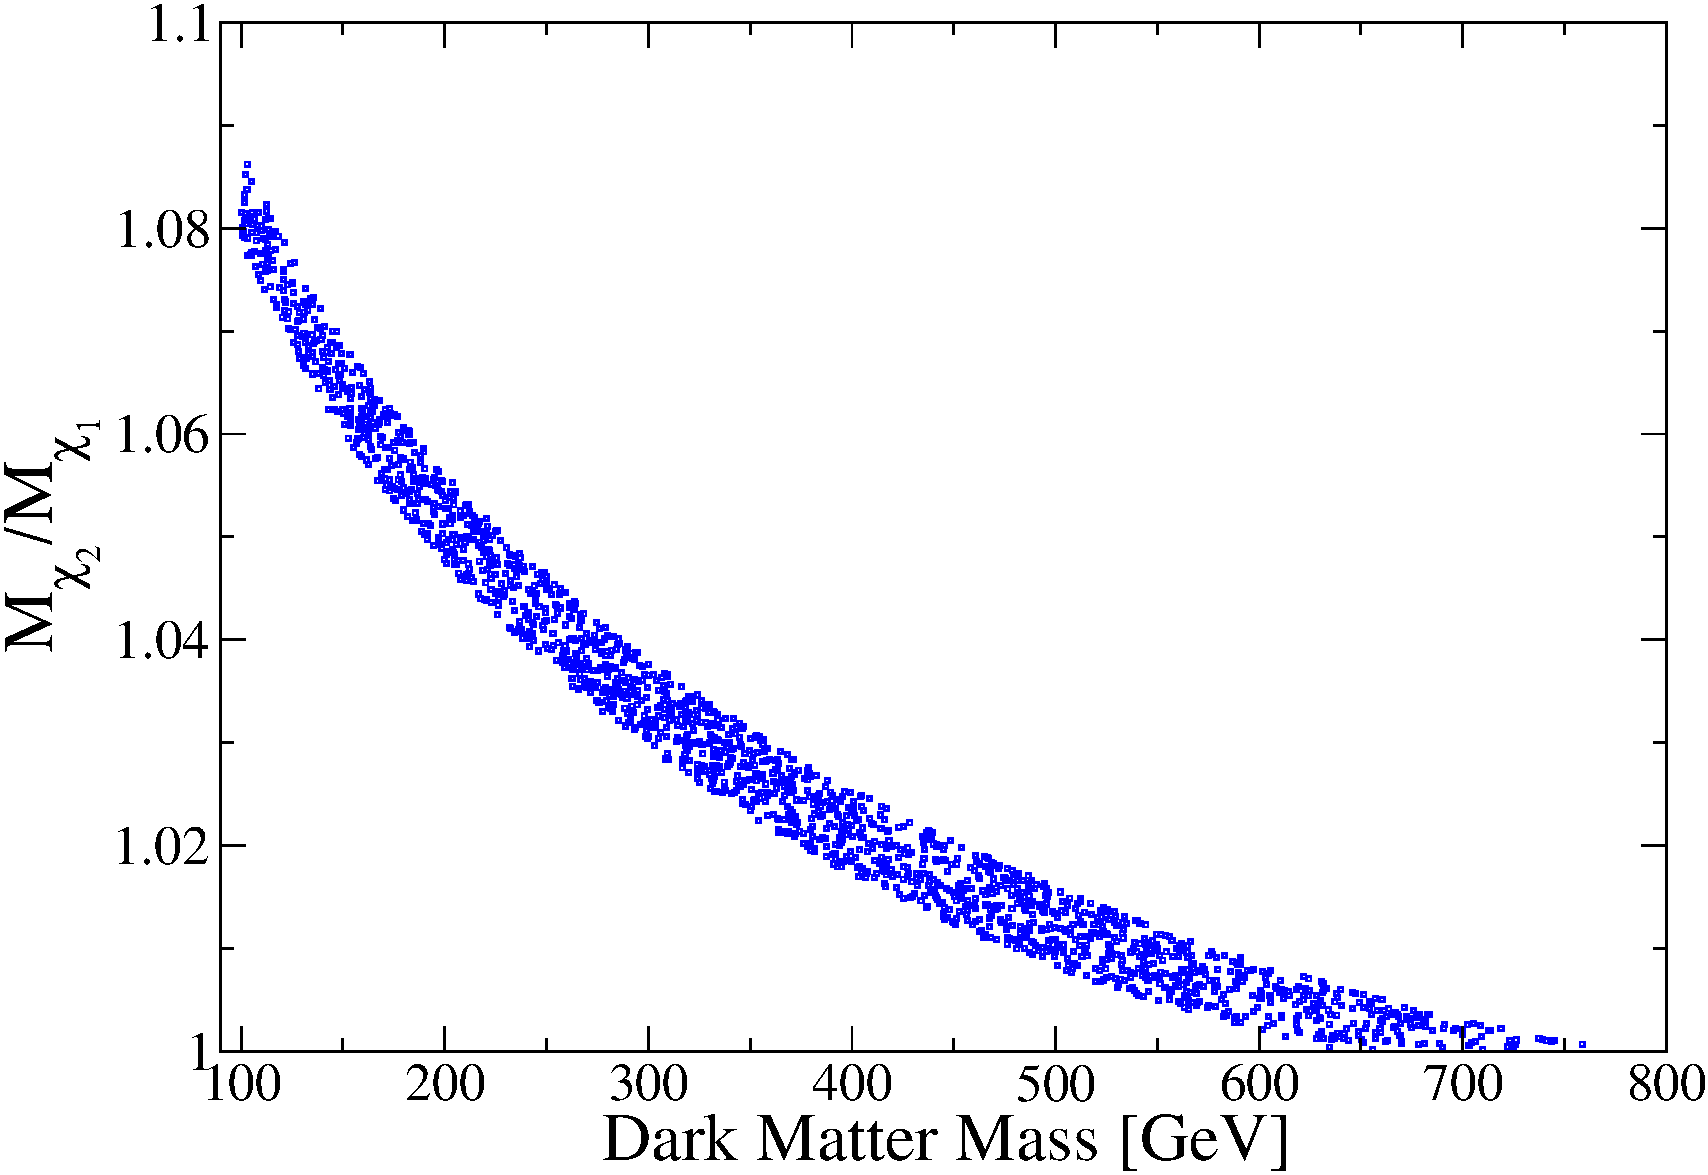
\includegraphics[scale=0.24]{coannmass}

    \hspace{2cm} Compressed spectra region
   \end{column}
    \begin{column}{0.5\textwidth}
      \includegraphics[scale=0.24]{ddsi}

      \only<1-2>{\hspace{2cm}LUX - XENON1T - LZ}
    \end{column}

  \end{columns}
  
  \invisible<1>{\includegraphics[scale=0.2]{llcom}}
  
  
\end{frame}


\begin{frame}
  \frametitle{Dark matter relic density}
  \begin{columns}
    \begin{column}{0.5\textwidth}
\includegraphics[scale=0.3]{S-channel}
\includegraphics[scale=0.3]{T-channel}
\includegraphics[scale=0.3]{U-channel}

\scriptsize Decoupled $Z'$ limit

\begin{align*}
\begin{pmatrix}
h \\ \operatorname{Re}(S)
\end{pmatrix} 
 =
\begin{pmatrix}
\cos\alpha & \sin\alpha \\
-\sin\alpha & \cos\alpha 
\end{pmatrix}
\begin{pmatrix}
h_1 \\ h_2
\end{pmatrix}\,.
\end{align*}
    \end{column}
    \begin{column}{0.5\textwidth}
\includegraphics[scale=0.4]{MSvsMD}

%\scriptsize Vector SI (blue points) and  scalar SI (green points)      
    \end{column}
  \end{columns}
\end{frame}


\begin{frame}
  \frametitle{Spin independent (SI) direct detection cross section}
  \begin{columns}
    \begin{column}{0.5\textwidth}
\includegraphics[scale=0.4]{vector-SI}
\includegraphics[scale=0.4]{scalar-SI}

\scriptsize Decoupled $Z'$ limit
    \end{column}
    \begin{column}{0.5\textwidth}
\includegraphics[scale=0.4]{SI}

%\scriptsize Vector SI (blue points) and  scalar SI (green points)      
    \end{column}
  \end{columns}
\end{frame}


\begin{frame}
\frametitle{Conclusions}
  It makes sense to focus our attention on models tha can account for neutrino masses and dark matter (DM) \alert{without adhoc symmetries}
\only<1>{
  \begin{block}{One-loop Dirac neutrino masses}
      A single $U(1)_X$ gauge symmetry to explain both the smallnes of Dirac neutrino masses and the stability of Dirac fermion dark matter
  %\setbeamercolor{block body}{use=structure,fg=black,bg=white}
    \begin{itemize}
    \item Spontaneously broken $U(1)_{X}$ generates a radiative Dirac neutrino masses
  \item A remnant symmetry makes the lightest field circulating the loop stable and good dark matter candidate.
  \item For T1-2-A: Either Singet Doublet Dirac Dark Matter or Singlet Scalar Dark Matter with extra scalar and vector portal
    \end{itemize}
  \end{block}
}

\end{frame}





{
\usebackgroundtemplate{\includegraphics[height=\paperheight]{silafaegua}}    
  \plain{
  \only<2>{\includegraphics[scale=0.9]{slfg}}
  
  Thanks!}
}
\end{document}


%slide with sm dirac fermion explanation
\begin{frame}
  \frametitle{Lepton number}
  \begin{itemize}
  \item   Lepton number ($L$) is an accidental discret or Abelian symmetry of the standard model (SM). 
  \item  Without neutrino masses $L_e$, $L_{\mu}$, $L_{\tau}$ are also conserved.
  \item The processes which violates individual $L$ are called Lepton flavor violation (LFV) processes.
  \item All the neutrino mass models predict, to some extent, LFV processes
  \item Only models with Majorana neutrinos predict processes with total $L=L_e+L_{\mu}+L_{\tau}$ violation, like \alert{neutrino less doublet beta decay} (NLDBD).
  \item NLDBD is experimentally challenging, specially if there is a massless neutrino in the spectrum.
  \end{itemize}
\end{frame}

%\end{document}
\begin{frame}
  \frametitle{NLDBD prospects for a  model with a massless
    neutrino \tiny (arXiv:1806.09977 [PLB] with Reig, Valle and Zapata) }
     \begin{figure}
      \centering
      \includegraphics[scale=0.25]{mee}\\
      {\tiny  with M.Reig, J.W.F Valle, O. Zapata, arXiv:1806.09977  }
    \end{figure}

 
\end{frame}


\begin{frame}
  \frametitle{Total lepton number: $L=L_e+L_{\mu}+L_{\tau}$}
  \begin{columns}
    \begin{column}{0.48\textwidth}
      \begin{block}{\centering Majorana $\cancel{\operatorname{U}(1)_L}$}
              \centering
    \rowcolors{1}{RoyalBlue!20}{}
\begin{tabular}{cc}
  Field &  $Z_2\ (\omega^2=1)$ \\\hline
  SM & $1$\\
  $L$& $\omega$ \\
     $ \left( e_R \right)^{\dagger}  $& $\omega$ \\
    $\left( \nu_R \right)^{\dagger}$ & $\omega$ \\\hline
    \end{tabular}

    \begin{align*}
      \mathcal{L}_{\nu}=h_D \left( \nu_R \right)^{\dagger}L \cdot H +
{\color{red}M_R\,\nu_R \nu_R}
      +\text{h.c}\,.
    \end{align*}
    \begin{align*}
      h_D \sim  \mathcal{O}(1) 
    \end{align*}
    \invisible<1->{Explain smallness ala Peccei-Quinn:
    \vspace{-0.5cm}
    \begin{align*}
      \operatorname{U}(1)_{B-L}\to Z_N\,,\quad N\ge 3\,.
    \end{align*}}    

      \end{block}
    \end{column}
  \begin{column}{0.48\textwidth}
    \begin{block}{\centering Dirac $\only<1>{\operatorname{U}(1)_L}
        \only<2>{\operatorname{U}(1)_{B-L}}$}
              \centering
    \rowcolors{1}{RoyalBlue!20}{}
\begin{tabular}{cc}
  Field &  $Z_3\ (\omega^3=1)$ \\\hline
  SM & $1$\\
  $L$& $\omega$ \\
       $ \left( e_R \right)^{\dagger}  $& $\omega^2$ \\
    $\left( \nu_R \right)^{\dagger}$ & $\omega^2$ \\\hline
    \end{tabular}

    \begin{align*}
      \mathcal{L}_{\nu}=h_D \left( \nu_R \right)^{\dagger}L \cdot H 
      +\text{h.c}\,.
    \end{align*}
    \begin{align*}
      h_D \sim \mathcal{O}(10^{-11}) 
    \end{align*}
    \invisible<1>{Explain smallness ala Peccei-Quinn:
      \vspace{-0.5cm}
    \begin{align*}
      \operatorname{U}(1)_{B-L} \underbrace{\longrightarrow}_{\color{red}\left\langle S \right\rangle} Z_N\,,\quad N\ge 3\,.
    \end{align*}}    
      \end{block}
    
  \end{column}
\end{columns}

\end{frame}



\begin{frame} 
  \frametitle{Small Dirac neutrino masses}
  \begin{columns}
    \begin{column}{0.78\textwidth}
      \small \qquad
      
      \vspace{0.2cm}
      
  To explain the \alert{smallness} of Dirac neutrino masses choose $\operatorname{U}(1)_{B-L} $ which:
  \begin{itemize}
  \item<1-> Forbids tree-level mass (TL) term ( $Y(H)=+1/2$ )
    \begin{align*}
      \mathcal{L}_{\text{T.L}}=&h_{D}\epsilon_{ab} \left( \nu_R \right)^{\dagger} L^a H^b +\text{h.c}\\
      =&h_D\left( \nu_R \right)^{\dagger} L\cdot  H +\text{h.c}\\
    \end{align*}
    \vspace{-1.5cm}
  \item<2-> Forbids Majorana term: $\nu_R \nu_R$
        \vspace{-0.3cm}
   \item<3-> Realizes of the 5-dimension operator which conserves lepton number in    $\operatorname{SU}(3)_c \times\operatorname{SU}(2)_L\times \operatorname{U}(1)_Y\times \operatorname{U}(1)_{B-L}$:
     \begin{align*}
       \mathcal{L}_{5-D}= \frac{h_\nu }{\Lambda}\left( \nu_R \right)^{\dagger} L\cdot H
       {\color{red}S}+\text{h.c}\\
     \end{align*}
             \vspace{-0.3cm}
           \item<4-> Enhancement to the \emph{effective number of degrees of freedom in the early Universe} $\Delta N_{\text{eff}}=N_{\text{eff}}-N_{\text{eff}}^{\text{SM}}$ ({\tiny see arXiv:1211.0186})             
  \end{itemize}

  \invisible<1-3>{See E. Ma, Rahul Srivastava: arXiv:1411.5042 [PLB] for tree-level realization} 
    \end{column}
    \begin{column}{0.22\textwidth}
      \invisible<1-2>{\includegraphics[scale=0.2]{l5d}}
    \end{column}
  \end{columns}

\end{frame}



\begin{frame}
\begin{picture}(320,250)
\only<1->{\put(-24,-22){\begin{overpic}[scale=0.352]{z2_bkg}\end{overpic}}}%
\only<1->{\put(34,158.5){ \textbf{SM}  }}%
\only<1->{\put(38,115){ {\large +}  }}%
\only<1->{\put(0,100){\Large $m^{\nu}_{\text{Majorana}}=\frac{1}{\Lambda} L \cdot H L \cdot H$   }}%
\only<1->{\put(-10,80){\Large $m^{\nu}_{\text{Dirac}}=\frac{1}{\Lambda} \left( \nu_R \right)^{\dagger}L \cdot H S$  }}%
%\only<2->{\put(2,80){ {\scriptsize This work, arXiv:1308.3655  [JHEP]} }}%
\only<1->{\put(18,115){\begin{overpic}[scale=0.118]{mice}\end{overpic}}}%
%
\only<2->{\put(240,180){\begin{overpic}[scale=0.15]{brickY}\end{overpic}}}%
\only<2->{\put(310,180){\begin{overpic}[scale=0.15]{brickR}\end{overpic}}}%
\only<2->{\put(380,180){\begin{overpic}[scale=0.15]{brickB}\end{overpic}}}%
\only<2->{\put(190,120){\begin{overpic}[scale=0.15]{brickG}\end{overpic}}}%
\only<2->{\put(260,120){\begin{overpic}[scale=0.15]{brickW}\end{overpic}}}%
\only<2->{\put(330,120){\begin{overpic}[scale=0.15]{brickK}\end{overpic}}}%
\only<2->{\put(120,40){ \begin{overpic}[scale=0.15]{brickssY}\end{overpic}}}%
\only<2->{\put(190,40){ \begin{overpic}[scale=0.15]{brickssR}\end{overpic}}}%
\only<2->{\put(260,40){ \begin{overpic}[scale=0.15]{brickssB}\end{overpic}}}%
\only<2->{\put(90,0){ \begin{overpic}[scale=0.15]{brickssG}\end{overpic}}}%
\only<2->{\put(160,0){ \begin{overpic}[scale=0.15]{brickssW}\end{overpic}}}%
\only<2->{\put(230,0){ \begin{overpic}[scale=0.15]{brickssK}\end{overpic}}}%
%\only<3->{\put(70,158){ \begin{overpic}[scale=0.27]{alert}\end{overpic}}}%
%\only<3->{\put(90,195){ {\huge \textbf{35 models}}  }}%
\end{picture}
\end{frame}


\end{document}

\begin{frame}
  \frametitle{\includegraphics[scale=0.1]{Q} \qquad Colored dark matter:
  \small De Luca , Mitridate, Redi, Smirnov \& Strumia, \tiny arXiv:1801.01135 [PRD]}

(Switch to Dirac fermions) \\
Because $\mathcal{Q}$ is a Dirac fermion, $\mathcal{Q} \mathcal{Q}$ is also stable
\begin{align*}
  \mathcal{Q}\mathcal{Q}\, \cancel{\to} &\, g\,, &\overline{\mathcal{Q}}\overline{\mathcal{Q}}\, \cancel{\to} &\, g\,.
\end{align*}

    \includegraphics[scale=0.09]{dmsteps}
  
\end{frame}


\begin{frame}
  \frametitle{Relic abundance. \footnotesize From: \url{http://bit.ly/Mitridate_53d_53rd_Rencontres_de_Moriond}  }
  \includegraphics[scale=0.3]{relden} 
\end{frame}

\begin{frame}
  \frametitle{Direct detection}
  \includegraphics[scale=0.52]{sigmaSI}
\end{frame}



\begin{frame}
  \frametitle{\only<1->{
    SD${}^{3}$M+$\sigma_i$ ($i=1,2$)     \invisible<2>{\scriptsize with J. Calle, C. Yaguna, and O. Zapata, arXiv:1812.05523 [PRD]  }  }}
\begin{picture}(320,250)
\only<1>{\put(-20,130){\tiny
        \begin{minipage}{0.3\linewidth}
          \begin{align*}
            \psi_{L,R}\to&\text{Singlet fermions \only<1>{(quiral)}  }\\
            \only<1>{\Psi_{L,R}\to&\text{Vector-like doublet fermions}\only<1>{:\qquad {\color{red}10/5}}   }\\
            \sigma\to&\text{Singlet scalar}\only<1->{:\qquad 15/5}   \\
            %\only<1>{\eta\to&\text{Doublet scalar}   }
          \end{align*}
        \end{minipage}
}}%
\only<1>{\put(190,135){\tiny
    \begin{minipage}{0.3\linewidth}
      \rowcolors{1}{RoyalBlue!20}{}
  \begin{tabular}{c|ccccccccc}\hline
 Fields: $f_i$  &  $\left( \nu_{R3} \right)^{\dagger}$
  &$\left( \nu_{R2} \right)^{\dagger}$&$\left( \nu_{R1} \right)^{\dagger}$&$\psi_L$&$\left( \psi_R \right)^{\dagger}$&$S$ &$\Psi_L$ & $\widetilde{\left( \Psi_R \right)}$& $\sigma$\\ \hline
    $\operatorname{U}(1)_{B-L}$ &$\displaystyle{+\frac{8}{5}}$&$\displaystyle{+\frac{8}{5}}$&$\displaystyle{+\frac{2}{5}}$&$\displaystyle{\frac{7}{5}}$&$\color{red}\displaystyle{-\frac{10}{5}}$&$\color{blue}\displaystyle{+\frac{3}{5}}$ &$\displaystyle{\frac{10}{5}}$ & $\displaystyle{-\frac{10}{5}}$  & $\displaystyle{\frac{7}{5}}$\\
    $\operatorname{SO}(10)$ &$16$ & $16$ & $16$ & $45$ & $45$ & $126$ & $10$ &$10$ & $16$ \\
  \end{tabular}
         \end{minipage}
       }}%
\only<1>{\put(250,95){\tiny
    \begin{minipage}{0.3\linewidth}
      \begin{center}
        Second Scotogenic Dirac from $\operatorname{SO}(10)$ E. Ma arXiv:1901.09091 [PLB]
       \end{center}
       \end{minipage}
       }}%
%  effective number of relativistic degrees of reedom Neff for neutrinos
% \only<4>{\put(40,20){\begin{overpic}[scale=0.6]{radiativedirac4}\end{overpic}}}%
 \only<1->{\put(40,20){\begin{overpic}[scale=0.6]{radiativedirac5}\end{overpic}}}%
 \only<2>{\put(20,200){
     \begin{minipage}{0.3\linewidth}
       $M_\psi=h_1 \left\langle S \right\rangle$, $\color{red}y_2=0$:
          \begin{align*}
            \mathcal{L}={\color{red}\mathcal{L}_{\text{SD${}^3$M}}}
            +{\color{Green} h_3^{ia} \widetilde{\left( \Psi_R \right)}\cdot L_i\, \sigma_a}+
      {\color{blue}      h_2^{\beta a} \left( \nu_{R\beta} \right)^{\dagger} \psi_L\, \sigma^{*}_a}
            -V(\sigma_a,S,H)\,.
          \end{align*}
        \end{minipage}
}}%
\only<2>{\put(0,130){\small with A.F Rivera, W. Tangarife,  arXiv:1906.09685   }}%
\only<2>{\put(220,60){\begin{overpic}[scale=0.6]{sarah}\end{overpic}}}%
\end{picture}
\end{frame}


% Now we introduce a vector like doublet
% From now on we will also decouple the Z'
% we end up with


\begin{frame}
  \frametitle{ Singlet-Doublet Dirac Dark Matter (SD${}^{3}$M)
By Carlos E. Yaguna.
arXiv:1510.06151 [PRD].
}

The model extends the standard model (SM) particle content with Dirac Fermions: from  $\operatorname{SU}(2)$ doublets of Weyl fermions: $\Psi_L=\left( \Psi_L^0,\, \Psi_L^-\right)^{\operatorname{T}}$, $\widetilde{\left( \Psi_R \right)}=\left( (\Psi_R^-)^\dagger,\, -(\Psi_R^0)^\dagger\right)^{\operatorname{T}}$  and singlet Weyl fermions $\psi_{LR}$ that interact among themselves and with the SM fields 
\begin{align}
  \mathcal{L}\supset& {\color{red} M_{\psi}}\left( \psi_R \right)^{\dagger}\psi_L
%+ {\color{red}h_S} \left( \psi_R \right)^{\dagger} \psi_LS  %+\text{h.c}.
%  \mathcal{L}_{\psi}+\mathcal{L}_{\sigma\psi}
+ %\left[
{\color{red}M_{\Psi}}\widetilde{\left( \Psi_R \right)}\cdot  \Psi_L
% +h_2^{ia} \widetilde{\left( \Psi_R \right)}\cdot L_i\, \sigma_a
+ {\color{red} y_1} \left( \psi_R \right)^{\dagger} \Psi_L \cdot H
+ {\color{red} y_2}  \widetilde{\left( \Psi_R \right)} \cdot \widetilde{H} \psi_L
                      +\text{h.c} % \right]
%+V(\sigma_a,S,H)\,,
\end{align}
Four free parameters:
\begin{align}
  {\color{red} M_{\psi}},{\color{red}M_{\Psi}}\ <& 2\text{ GeV}\,,&
  {\color{red} y_1},\ {\color{red} y_2} > 10^{-6}
\end{align}
Two neutral Dirac fermion eigenstates:
\begin{align}
  M=&
  \begin{pmatrix}
    {\color{red}M_{\psi}} & {\color{red}y_{2}} v/\sqrt{2} \\ {\color{red}y_{1}} v/\sqrt{2} & {\color{red} M_{D}}
  \end{pmatrix},&
M_{\text{diag}}=&
\begin{pmatrix}
{M_{\chi_{1}}} & {0} \\ {0} & {M_{\chi_{2}}}                    
\end{pmatrix}
=U_{L}^{\dagger} M U_{R}
\end{align}


\end{frame}


\begin{frame}
    \frametitle{ SD${}^{3}$M
By Carlos E. Yaguna.
arXiv:1510.06151 [PRD].
}
    \begin{columns}
    \begin{column}{0.5\textwidth}
      \includegraphics[scale=0.24]{coannmass}

    \hspace{2cm} Compressed spectra region
   \end{column}
    \begin{column}{0.5\textwidth}
      \includegraphics[scale=0.24]{ddsi}

      \only<1-2>{\hspace{2cm}LUX - XENON1T - LZ}
    \end{column}

  \end{columns}
  
  \invisible<1>{\includegraphics[scale=0.2]{llcom}}
  
  
\end{frame}


\begin{frame}
  \frametitle{Spin independent (SI) direct detection cross section}
  \begin{columns}
    \begin{column}{0.5\textwidth}
      
\includegraphics[scale=0.4]{vector-SI}
\includegraphics[scale=0.4]{scalar-SI}

\scriptsize Decoupled $Z'$ limit
    \end{column}
    \begin{column}{0.5\textwidth}
\includegraphics[scale=0.4]{MSvsMD}

\scriptsize Vector SI (blue points) and  scalar SI (green points)      
    \end{column}
  \end{columns}
\end{frame}

%\begin{frame}
%   \frametitle{SM-like $B-L$ model}
%  \begin{center}
%     \rowcolors{1}{RoyalBlue!20}{}
%  \begin{tabular}{lr}
%    Field & $\operatorname{U}(1)_{B-L}$ \\ \hline
%    $L$   & -1\\
%    $H$   & 0\\
%    $S$   & $s$\\
%    $\left( \psi_R \right)^{\dagger}_\alpha$ & $\color{red}r_{\alpha}$\footnote{Weyl notation with only left-handed fields defined; $\color{red}r_{\alpha}$ restricted by anomaly cancellation}\\
%  \end{tabular}
% \end{center}

% \begin{block}{Massless Majorana fermions ($n=0,1$)}
%   \begin{align*}
%     L \left[ \left( \psi_R \right)^{\dagger}_\alpha \left( \psi_R \right)^{\dagger}_\beta S^n \right]  \Longrightarrow& {\color{red} r_{\alpha}+r_{\beta}}+nS\ne 0\,,
%    & &\text{example: $\color{red}r\ne 1$, if $s=-2$}\,.
%   \end{align*}
% \end{block}

%  \vspace{-0.5cm}
% \setbeamercolor{block title}{bg=yellow!30,fg=black}
%  \begin{varblock}[\textwidth]{  $\operatorname{U}(1)_{B-L}$ with 3+$\alpha$ zero Majorana Masses $\iff$ SM with 3 zero Majorana masses }      
%  \end{varblock}

% \vspace{-0.8cm}
%  \begin{align*}
% \text{ For $\alpha\le 2$: }   \left( \psi_R \right)^{\dagger}_\alpha\to &\left( \nu_R \right)^{\dagger}_\alpha&
%           \color{red} r_{\alpha}\to & \color{Green} \nu_{\alpha}
%  \end{align*}


 

 
% \end{frame}

%\end{document}

% \begin{frame}
%   \frametitle{Majorana vs Dirac}
%   \begin{columns}
%     \begin{column}{0,5\textwidth}
%       Majorana\\
%       5-dimensional 
%       \begin{align*}
        
%       \end{align*}
%     \end{column}
%     \begin{column}{0,5\textwidth}
%       Dirac \\
%     \end{column}
%   \end{columns}
% \end{frame}


% \section{(Dirac) Neutrino masses}


% \begin{frame}
%   \frametitle{Seesaw mechanism}

%  For Dirac neutrino masses: we require to introduce at least one SM-singlet heavy Dirac fermión (Weyl fermion notation)
%  \begin{align}
%    \mathcal{L}=i\, \left( \psi _L \right)^{\dagger}\overline{\sigma}^{\mu}\partial_{\mu}\psi_L -m \,\left( \psi _R \right)^{\dagger}\psi_L+\text{h.c}\,.
%  \end{align}


%  \begin{center}
%     \rowcolors{1}{RoyalBlue!20}{}
%  \begin{tabular}{lr}
%    Field & $\operatorname{U}(1)_{B-L}$ \\ \hline
%    $L$   & -1\\
%    $H$   & 0\\
%       $S$   & $s$\\
%    $\left( \nu_R \right)^{\dagger}_i$ & $\color{Green}\nu_i$\\
%    $\left( \psi_R \right)^{\dagger}$ & $\color{red}r$\\
%   $\psi_L$ & $\color{red}-r$\\ \hline
%  \end{tabular}
%  \end{center}

% If  $\left( \psi_R \right)^{\dagger}_{\alpha}$  can couple with $\left( \psi_R \right)^{\dagger}_{\beta} $, then  $\left( \psi_R \right)^{\dagger}_{\beta}\to {\psi_L}_{\alpha}$, 
 
% \end{frame}


% \begin{frame}
%   \frametitle{
%     \only<1>{T3-1-A}%
%     \only<2>{Exotic $\left( \nu_R \right)^{\dagger}$ with $\nu\ne-1$,
%      and vector-like Dirac fermion with $r\ne 1$}%
%    %\only<5>{The model: \textit{colored scotogenic}}%
%   }
% \def\pscale{0.6}
% \def\px{0}
% \def\py{140}
% \begin{picture}(320,250)
% \only<1-2>{\put(\px,\py){%\includegraphics[scale=\pscale]{dm3}
%     \begin{overpic}[scale=\pscale]{dm3}
%     \end{overpic}
%   }}%
% %\only<5>{\put(\px,\py){\includegraphics[scale=\pscale]{dm4}}}%
% %%% circle
% \FPeval\vx{\px+52}%
% \FPeval\vy{\py+3}%
% \only<2>{\put(\vx,\vy){\tikz \draw[red,thick,rounded corners] (0,0) rectangle (0.5,0.5);} }
% \FPeval\vxr{\vx+73}%
% \only<2>{\put(\vxr,\vy){\tikz \draw[red,thick,rounded corners] (0,0) rectangle (0.5,0.5);} }
% \FPeval\vxr{\vx+\vy}%
% \only<2>{\put(\vxr,\vy){\tikz \draw[red,thick,rounded corners] (0,0) rectangle (0.5,0.5);} }
% \FPeval\vxr{\vx+73}%
% \FPeval\vyr{\vy+58}%
% \only<2>{\put(\vxr,\vyr){\tikz \draw[red,thick,rounded corners] (0,0) rectangle (0.5,0.5);} }
% \FPeval\sx{\px+270}%
% \FPeval\sy{\py+60}%
% \only<1->{\put(\sx,\sy){
%     \begin{minipage}{0.4\linewidth}
%       \begin{block}{Soft breaking term induced:}
%     \begin{align*}
%       \mathcal{L}\supset & \kappa  \sigma \eta^{\dagger} H\,,
%     \end{align*}
%     %\invisible<5>
%     {where $\kappa=\lambda \langle S \rangle\,.$}
    
%       \end{block}
%   \end{minipage}
%   }}
% \only<2->{\put(0,80){
%     \begin{columns}
%       \begin{column}{0.55\textwidth}
%         \begin{align*}
%           -1+\eta=&-\color{red}r\\
%           -{\color{red}r}=&-\color{red}r\\
%           -{\color{red}r}=&-{\color{Green}\nu}+\sigma\\
%           \sigma=&\eta+s
%         \end{align*}
%         \begin{align*}
%           \only<2>{\boldsymbol{N}_c=\boldsymbol{1}\,.}%
%           %\only<5>{\color{red}\boldsymbol{N}_c=\boldsymbol{8}\,.}%
%         \end{align*}
%       \end{column}
%       \begin{column}{0.45\textwidth}

%         \rowcolors{1}{RoyalBlue!20}{}
%         \small
%   \begin{tabular}{|l|c|l|c|}
% \hline
%     Particles& $\operatorname{U}(1)_{B-L}$ & $\left(\operatorname{SU}(3)_c ,\operatorname{SU}(2)_L \right)_Y$\\\hline
%     $L_i$                           & $\color{blue}-1$ & $ \left(\mathbf{1},\mathbf{2}\right)_{-1/2}$  \\
%  $H$                           &          0  & $ \left(\mathbf{1},\mathbf{2}\right)_{1/2}$ \\     
%  $\left( \nu_{Ri} \right)^{\dagger}$ & $\color{Green}\nu$ & $ \left(\mathbf{1},\mathbf{1}\right)_0$ \\ 
%     \only<2>{$\psi_L$}%
%     %\only<5->{$\color{red}\mathcal{Q}_L$}
%              & $\color{red}-r$ &
%     $ \left(\only<2>{\mathbf{N}_c}
%             %\only<5>{{\color{red}\mathbf{N}_c}}
%             ,\mathbf{1}\right)_0$\\
%     \only<2>{$\left( \psi_R \right)^{\dagger}$}%
%     %\only<5->{$\color{red}\left( \mathcal{Q}_R \right)^{\dagger}$}
%              & $\color{red}r$ &
%                                 $ \left(\only<2>{\mathbf{N}_c}
%                                 %\only<5>{{\color{red}\mathbf{N}_c}}
%                                 ,\mathbf{1}\right)_0$ \\
%     $\sigma_a$                           &  ${\color{Green}\nu}-\color{red}r$   &
%                                                                                   $ \left(\only<2>{\mathbf{N}_c}
%                                                                                   %\only<5>{{\color{red}\mathbf{N}_c}}
%                                                                                   ,\mathbf{1}\right)_0$ \\
%     $\eta_a$                        &  $1-\color{red}r$   &
%                                                             $ \left(\only<2>{\mathbf{N}_c}
%                                                             %\only<5>{{\color{red}\mathbf{N}_c}}
%                                                             ,\mathbf{2}\right)_{1/2}$ \\
%     % \invisible<5>
%     {$S$}&
%     % \invisible<5>
%            { ${\color{Green}\nu}-1$ }  &
%     %\invisible<5>
%     { $\left(\mathbf{N}_c,\mathbf{2}\right)_{1/2}$ }\\  
%   \end{tabular}

        
%       \end{column}
%     \end{columns}
%   }}
% \end{picture}

  
% \end{frame}




% \begin{frame}
%   \frametitle{Neutrino masses and mixings}
%   \begin{itemize}
%   \item<1->  $\nu_i$ are free parameter and could be fixed if we impose $\operatorname{U}(1)_{B-L}$ to be local
%   \begin{align*}
%    \color{red} r\ne&\color{red}1\,, & \sum_i   \color{Green} \nu_i =&3\,, & \sum_i \color{Green} \nu_i^3 =&3 
%   \end{align*}


%   \begin{center}
%       \rowcolors{1}{RoyalBlue!20}{}    
%   \begin{tabular}{rlll}
%     & $\left( \nu_R \right)^{\dagger}_1$ & $\left( \nu_R \right)^{\dagger}_2$ & $\left( \nu_R \right)^{\dagger}_3$ \\
%     $\operatorname{U}(1)_{B-L}$ &$+4$& $+4$& $-5$\\
%     $\operatorname{U}(1)_{B-L}$ &$-6$& $+\dfrac{10}{3}$& $+\dfrac{17}{3}$\\
%   \end{tabular}
%     \end{center}
  
%   \item<2-> To have at least a rank 2 neutrino mass matrix we need either:
%   \begin{itemize}
%   \item At least two heavy Dirac fermions $\Psi_a$, $a=1,2,\ldots$
%   \item \only<2>{At least two sets of scalars $\eta_a$, $\sigma_a$}%
%     \only<3->{\color{red}At least two sets of scalars $\eta_a$, $\sigma_a$}%
%   \end{itemize}
% \item<4> 
%   \begin{align*}
%     \mathcal{L}\supset&\left[ {\color{red}  M_{\Psi}\, \left( \psi_R \right)^{\dagger} \psi_L}
%        + h^{a}_i   \left( \psi_R \right)^{\dagger} \widetilde{\eta}^\dagger_a L_i
%   +y^a_i    \overline{\nu_{Ri} }\  \sigma_a^{*} \psi_L  +\text{h.c}\right]
% +\kappa^{ab}\, \sigma_a \eta_b^{\dagger} H+\ldots
%   \end{align*}
  
%   \end{itemize}

  
% \end{frame}


% \begin{frame}
%   \frametitle{Neutrino masses and mixings {\tiny  (with M.Reig, J.W.F Valle, O. Zapata, arXiv:1806.09977 ) }}
%   %
% \begin{align}
% \left(\mathcal{M}_\nu\right)_{ij}=&N_c\frac{M_{\Psi}}{64\pi^2}\sum_{a=1}^2h_{i}^a y_{j}^a\frac{\sqrt{2}\kappa_{aa}v}{m^2_{S_{2R}^a}-m^2_{S_{1R}^a}}
%   \left[F\left(\frac{m^2_{S_{2R}^a}}{M_{\Psi}^2}\right)-F\left(\frac{m^2_{S_{1R}^a}}{M_{\Psi}^2}\right)\right]+(R\to  I)
% \end{align}
% %
% where
% $F(m_{S_\beta}^2/M_\Psi^2)=m_{S_\beta}^2\log(m_{S_\beta}^2/M_\Psi^2)/(m_{S_\beta}^2-M_\Psi^2)$. The four CP-even mass eigenstates are denoted as
% $S_{1R}^1,S_{2R}^1,S_{1R}^2,S_{2R}^2$, with a similar notation for the
% CP-odd ones.

% % If $(\mu_\eta^{aa})^2\gg M_{\Psi}^2$ one has
% % \begin{align}
% %  &\left(\mathcal{M}_\nu\right)_{ij}=N_c\frac{M_{\Psi}}{32\pi^2}\sqrt{2}v\sum_{a=1}^2\kappa^{aa}\frac{h_{i}^a y_{j}^a}{(\mu_\eta^{aa})^2}\\
% %  &\sim 0.03\,\mbox{eV}\left(\frac{M_{\Psi}}{12.5\, \mbox{TeV}}\right)\left(\frac{\kappa^{aa}}{1\, \mbox{GeV}}\right)\left(\frac{50\,\mbox{TeV}}{\mu_\eta^{aa}}\right)^2\left(\frac{h_{i}^a y_{j}^a}{10^{-6}}\right).\nonumber
% % %
% % \end{align}
% %


% \end{frame}



% \begin{frame}
%   \frametitle{T3-1-A with only $U(1)_{B-L}$}
%   % 1805.02025 Han, Wang extra $Z_2$
  
%   \begin{columns}
%   \begin{column}{0.28\textwidth}
% \rowcolors{1}{RoyalBlue!20}{}
%     \begin{tabular}{ll}
%       Field &  $\operatorname{U}(1)_{B-L}$ \\\hline
%       $\left( \nu_{R_i} \right)^{\dagger}$ & $+4$ \\
%       $\left( \nu_{R_j} \right)^{\dagger}$ & $+4$ \\
%       $\left( \nu_{R_k} \right)^{\dagger}$ & $-5$ \\  
%       $\color{red}\psi_L$ & $\color{red}-r$ \\
%       $\color{red}\left( \psi_R \right)^{\dagger}$ &\color{red} $r$ \\\hline
%       $\color{red}\eta_a$ &\color{red} $r{\color{black}-4}$ \\\hline
%       $\color{red}\sigma_a$ &\color{red} $r{\color{black}-1}$ \\
%       $S$ & $-3$ \\
%     \end{tabular}
%     \small 
%     $a=1,2$, $i\ne j\ne k$.\\
%     $m=0$: $\nu_{L_k}$, and $\nu_{R_k}\to N_{\text{eff}}$
%     \begin{align*}
%       F_1=
%       \begin{pmatrix}
%         \psi_L\\
%         \psi_R\\
%       \end{pmatrix}
%     \end{align*}
%   \end{column}
%   \begin{column}{0.62\textwidth}

%     \begin{figure}
%       \centering
%       \only<1>{\includegraphics[scale=0.8]{FgZ-2}}
%       \only<2>{\includegraphics[scale=0.8]{FDM}}\\
%       {\tiny Extra $Z_2$:   Han, Wang,  1808.03352 [EJPC]  }
%     \end{figure}


    
%   \end{column}
% \end{columns}
  
%   %\includegraphics{}
% \end{frame}

\begin{frame}
  \frametitle{Dirac neutrinos in LR }
  see E.Ma and U. Sarkar, arXiv:1707.07698 [PLB]
\end{frame}


{
%\usebackgroundtemplate{\includegraphics[width=\paperwidth]{explosion}}  
\begin{frame}
  \frametitle{Conclusions}

  A single $U(1)$ symmetry to explain both the smallnes of  neutrino masses and the stability of fermion dark matter
  %\setbeamercolor{block body}{use=structure,fg=black,bg=white}

  \begin{block}<2>{Neutrino masses and DM}
    \begin{itemize}
    \item Spontaneously broken $U(1)_{X}$ generates a radiative  neutrino masses
  \item A remnant symmetry makes the lightest field circulating the loop stable and good dark matter candidate.
  \item For T1-2-A: Either Singet Doublet (Dirac) Dark Matter or Singlet Scalar Dark Matter with extra scalar and vector portal
  \item With relaxed direct detection constraints
    \end{itemize}
  \end{block}
\end{frame}
}

\plain{Thanks!}
\end{document}

\section{radiative seesaw}
\begin{frame}
\frametitle{Radiative seesaw}
\begin{picture}(320,250)
\only<1->{\put(-24,-17){\begin{overpic}[scale=0.352]{z2_bkg}\end{overpic}}}%
\only<1->{\put(180,20){\begin{overpic}[scale=0.25]{type1}\end{overpic}}}%
\only<1->{\put(-10,120){\includegraphics[scale=1]{T3_a}}}%
\only<1->{\put(2,80){ {\scriptsize E. Ma, hep-ph/0601225 [PRD]} }}%

\end{picture}
\end{frame}

\section{Inert doublet model}


\begin{frame}
  \frametitle{Inert doublet model}

  The Lagrangian of the model is given by:
\begin{align}
\label{eq:0001}
\mathcal{L} =\mathcal{L}_{\text{SM}}+ (D^{\mu}{\color{red}\Phi})^{\dagger} D_{\mu}{\color{red}\Phi} -V({\color{red}\Phi}),
\end{align}
where
\begin{align}
\label{eq:0002}
V({\color{red}\Phi}) =& \mu_2^{2} {\color{red}\Phi}^{\dagger}{\color{red}\Phi} + \lambda_2 ({\color{red}\Phi}^{\dagger}{\color{red}\Phi})^{2} + 
\lambda_3 (H^{\dagger}H)({\color{red}\Phi}^{\dagger}{\color{red}\Phi})  + \lambda_4 (H^{\dagger}{\color{red}\Phi})({\color{red}\Phi}^{\dagger}H) + \dfrac{\lambda_5}{2} \Big [ ({\color{red}\Phi}^{\dagger}H)^2 + \text{h.c.} \Big ].
\end{align} 
$H$ os the SM Higgs doublet in the SM,
We define
\begin{align}
\lambda_L=\frac{\lambda_3+\lambda_4+\lambda_5}{2}\,.
\end{align}
which controls the interactions though the Higgs portal. The components  are

\begin{align*}
\label{eq:0003}
{\color{red}\Phi}=\begin{pmatrix}
\color{red} H^{+} \\
\dfrac{1}{\sqrt{2}}( {\color{red}H^{0} + i A^{0}}) 
\end{pmatrix}, \hspace{2cm}
H=\begin{pmatrix}
 G^{+} \\
\dfrac{1}{\sqrt{2}}(v + h^{0} + i G^{0}) 
\end{pmatrix}.
\end{align*}

\alert{%Multilepton signals reach for thermal
  Drell-Yann production for $m_{H^0}\approx 60\ \text{GeV}$, can prove $m_{H^+}\sim 150\ \text{GeV}$.} 

  
\end{frame}

\begin{frame}
  \frametitle{Vector Boson Fussion}
\def\sep{\hspace{0.3cm}}
\def\scl{0.18}
\begin{center}
    \includegraphics[scale=\scl]{vbf_a}\sep
\includegraphics[scale=\scl]{vbf_z}\sep
\includegraphics[scale=\scl]{vbf_zh}\sep
\includegraphics[scale=\scl]{vbf_gh}
\end{center}


\end{frame}

\begin{frame}
  \frametitle{$\sigma=B/\sqrt{B+S}$}
 \begin{table}
 \centering
 \begin{tabular}{|c|c|c|c|}\hline
 $\lambda_L$& $S_{\text{MJ}}$ & $B_{\text{MJ}}$ & $\sigma_{\text{MJ}}$ \\\hline
 0.01 & 3 &  & 0.015 \\ %  old
 0.1 & 3.7 & 134044 & 0.02 \\ % old
 1.0 & 31 & & 0.15\\ \hline % old
 \end{tabular}\hspace{1cm}
 \begin{tabular}{|c|c|c|c|}\hline
 $\lambda_L$& $S_{\text{VBF}}$ & $B_{\text{VBF}}$ & $\sigma_{\text{VBF}}$ \\\hline
 0.01 & 4.6 &  & 0.21 \\
 0.1 & 7.5 & 476 & 0.35 \\
 1.0 & 25 & & 1.1\\  \hline
 \end{tabular}

 \caption{Sensitivities for $M_{H^+}=M_{A^0}=750\ $GeV and $M_{H_0}=110\ $GeV for several  $\lambda_L$ values, with an integrated luminosity of $20$~fb$^{-1}$.}
% %The Monojet results were obtained with CheckMate.}
% \label{tab:monjet-VBF}
\end{table}
  
\end{frame}


\begin{frame}
  \frametitle{3 $\sigma$ reach }
  \begin{picture}(320,250)
    \only<1->{\put(-24,37){\begin{overpic}[scale=0.5]{lc3}\end{overpic}}}%
    \only<2->{\put(260,220){\alert{$\Omega_{H^{0}}\ll \Omega_{\text{DM}} $} }}%
    \only<1->{\put(260,140){$m_{H^+}=m_{A^0}=600\ \text{GeV}$ }}%
    \only<2->{\put(260,80){\alert{$\Omega_{H^{0}}\sim \Omega_{\text{DM}} $} for $m_{H^{0}}\sim 60\ \text{GeV}$}}%
  \end{picture}


\end{frame}




\begin{frame}
\frametitle{Weinberg operator at one-loop}
\begin{picture}(320,250)
\only<1->{\put(-20,140){\includegraphics[scale=0.8]{T3}}}%
\only<1->{\put(160,140){\includegraphics[scale=0.8]{T1-2}}}%
\only<1->{\put(-20,20){\includegraphics[scale=0.8]{T1-1}}}%
\only<1->{\put(160,20){\includegraphics[scale=0.8]{T1-3}}}%
\only<1->{\put(-20,130){Bino/Wino-like scotogenic model}}
\only<3->{\put(150,13){\includegraphics[scale=0.1]{new}Higgsino-like scotogenic model}}
\only<3->{\put(150,130){\includegraphics[scale=0.1]{new}Higgsino-like Zee model}}
\only<3->{\put(55,118){$\Updownarrow$}}
\only<1->{\put(40,160){\tiny arXiv:1605.01129}}
\only<3->{\put(225,160){\tiny arXiv:1511.01873}}
\only<3->{\put(225,40){\tiny arXiv:1504.07892}}
\only<1->{\put(120,240){\color{red}($Z_2$-odd fields) }}
\only<2->{\put(340,120){\includegraphics[scale=0.8]{main_vertex4}}}%
\only<2->{\put(360,100){ $pp\to l^+l^-+{E_T^{\text{miss}}}$  }}%
\only<2->{\put(360,50){ $\mu\to e \gamma,\ \ldots$   }}%
%\only<4->{\put(233,186){\fcolorbox{black}{blue}{\color{white}Zee model}}}%
\end{picture}
\end{frame}


\section{Inverse radiative seesaw}
\begin{frame}
\frametitle{Inverse radiative seesaw}  
\begin{picture}(320,250)
\only<1->{\put(-24,-17){\begin{overpic}[scale=0.352]{z2_bkg}\end{overpic}}}%
\only<1->{\put(200,20){\begin{overpic}[scale=0.25]{inverse_type1}\end{overpic}}}%
\only<1->{\put(-10,120){\includegraphics[scale=1]{T1-3_a}}}%
\only<1->{\put(2,80){ {\scriptsize D.R \emph{et al}, arXiv:1504.07892 [PRD]} }}%

\end{picture}
\end{frame}

\section{Singlet-doublet fermion dark matter}
\begin{frame}
  \frametitle{Singlet-doublet fermion dark matter}

  \begin{center}
\rowcolors{1}{RoyalBlue!20}{}
%\def\arraystretch{1.1}
   \begin{tabular}{llllll}
 $\text{Name}$ &  $\text{SU}(3)_c$ & $\text{SU}(2)_L $& $\text{U}(1)_Y$ & $Z_2$ \\ \hline
 $L=(\nu_L  \  e_L)^{\operatorname{T}}$ &  $ \mathbf{1} $ & $ \mathbf{2} $ & $ -1/2 $ & $ +1$\\
$(e_R)^{\dagger} $ &  $ \mathbf{1} $ & $ \mathbf{1} $ & $ +1 $ & $ +1$ \\
     \color{red} $ ({\hat\Psi}_R)^{\dagger}
     =\left( \left( \psi_R^+ \right)^{\dagger} \ 
     {\color{blue} \left( \psi_R^0 \right)^{\dagger}}
     \right)^{\operatorname{T}}
     $ &  $ \mathbf{1} $ & $ \mathbf{2} $ & $ +1/2 $ & $ \color{red} -1$ \\
     \color{red} $\Psi_L=\left( {\color{blue}\psi_L^0} \ \psi_L^-
     \right)^{\operatorname{T}}$
&   $ \mathbf{1} $ & $ \mathbf{2} $ & $ -1/2 $ & $\color{red} -1$ \\
 $ {\color{blue}N} $ &  $ \mathbf{1} $ & $ \mathbf{1} $ & $ 0 $ & $\color{red} -1$ \\
\color{red} $S$ &   $ \mathbf{1} $ & $ \mathbf{1} $ & $ 0 $ & $\color{red} -1$ \\
 \end{tabular}
  \end{center}

\begin{columns}
  \begin{column}{0.33\textwidth}
\includegraphics[scale=0.5]{hpf}    
  \end{column}
  \begin{column}{0.33\textwidth}
Basis $\boldsymbol{\psi}^0=\left({\color{blue}N},{\color{blue}\psi_L^0},{\color{blue}\left( \psi_R^0 \right)^{\dagger}}\right)^T$ 
\tiny
\begin{align*}
  &\mathcal{M}_{\boldsymbol{\psi}^0}=\nonumber\\
&\begin{pmatrix}
{\color{blue}M_N}               &{\color{blue}-y\,c_\beta v/\sqrt{2}}&{\color{blue}y\,s_\beta v/\sqrt{2}} \\
{\color{blue}-y\,c_\beta} v/\sqrt{2}  & 0            & {\color{blue}}-M_D\\
{\color{blue}y\,s_\beta v/\sqrt{2}} &{\color{blue}}  -M_D                &  0  \\
\end{pmatrix},
\end{align*}
    
  \end{column}
  \begin{column}{0.33\textwidth}
    \only<1>{\includegraphics[scale=0.2]{GCE}}\only<2->{\includegraphics[scale=0.2]{GCE2016}}%
{\tiny S. Horiuchi,\\ O. Macias, DR, A. Rivera, O. Zapata, 1602.04788 (JCAP) }
  \end{column}
\end{columns}

\end{frame}


\section{Singlet scalar dark matter}
\begin{frame}
  \frametitle{Scalar dark matter: Higgs portal}

  \begin{center}
\rowcolors{1}{RoyalBlue!20}{}
%\def\arraystretch{1.1}
   \begin{tabular}{llllll}
 $\text{Name}$ &  $\text{SU}(3)_c$ & $\text{SU}(2)_L $& $\text{U}(1)_Y$ & $Z_2$ \\ \hline
 $L=(\nu_L  \  e_L)^{\operatorname{T}}$ &  $ \mathbf{1} $ & $ \mathbf{2} $ & $ -1/2 $ & $ +1$\\
$(e_R)^{\dagger} $ &  $ \mathbf{1} $ & $ \mathbf{1} $ & $ +1 $ & $ +1$ \\
     \color{red} $ ({\hat\Psi}_R)^{\dagger}
     =\left( \left( \psi_R^+ \right)^{\dagger} \ 
     {\color{blue} \left( \psi_R^0 \right)^{\dagger}}
     \right)^{\operatorname{T}}
     $ &  $ \mathbf{1} $ & $ \mathbf{2} $ & $ +1/2 $ & $ \color{red} -1$ \\
     \color{red} $\Psi_L=\left( {\color{blue}\psi_L^0} \ \psi_L^-
     \right)^{\operatorname{T}}$
&   $ \mathbf{1} $ & $ \mathbf{2} $ & $ -1/2 $ & $\color{red} -1$ \\
 $ {\color{blue}N}\hspace{-0.28cm}{\color{red}N} $ &  $ \mathbf{1} $ & $ \mathbf{1} $ & $ 0 $ & $\color{red} -1$ \\
\color{red} $S$ &   $ \mathbf{1} $ & $ \mathbf{1} $ & $ 0 $ & $\color{red} -1$ \\
 \end{tabular}
  \end{center}

 % \includegraphics[scale=0.5]{hp}
 \begin{columns}
  \begin{column}{0.33\textwidth}
\includegraphics[scale=0.5]{hp}    
  \end{column}
  \begin{column}{0.67\textwidth}
    % \small
     \begin{align*}
   \mathcal{V}=&  M_{S}^2 {\color{red} S^2}+ \lambda_{SH}{\color{red} S^2}\, \widetilde{H}\cdot H + \lambda_S {\color{red} S^4}
     \end{align*}
     \vspace{-1cm}
\begin{align*}
  \lambda_{HS}\sim
  \begin{cases}
    0.1 & \text{WIMP} \\ %refs
    10^{-9} & \text{FIMP}+\text{$\color{red}S$inflaton (Tenkanen) } \\ %refs
  \end{cases}
\end{align*}
   Tenkanen. arXiv:1607.01379 (JHEP) 
  \end{column}
\end{columns}

\end{frame}





\begin{frame}
  \frametitle{Scalar dark matter: vector-like fermion portal}
  \begin{center}
\rowcolors{1}{RoyalBlue!20}{}
%\def\arraystretch{1.1}
   \begin{tabular}{llllll}
 $\text{Name}$ &  $\text{SU}(3)_c$ & $\text{SU}(2)_L $& $\text{U}(1)_Y$ & $Z_2$ \\ \hline
 $L=(\nu_L  \  e_L)^{\operatorname{T}}$ &  $ \mathbf{1} $ & $ \mathbf{2} $ & $ -1/2 $ & $ +1$\\
$(e_R)^{\dagger} $ &  $ \mathbf{1} $ & $ \mathbf{1} $ & $ +1 $ & $ +1$ \\
\color{red} $ (\psi_R^-)^{\dagger} $ &  $ \mathbf{1} $ & $ \mathbf{1} $ & $ +1 $ & $ \color{red} -1$ \\
\color{red} $\psi_L^- $ &  $ \mathbf{1} $ & $ \mathbf{1} $ & $ -1 $ & $\color{red} -1$ \\
\color{red} $S$ &   $ \mathbf{1} $ & $ \mathbf{1} $ & $ 0 $ & $\color{red} -1$ \\
 \end{tabular}
  \end{center}


\begin{columns}
  \begin{column}{0.15\textwidth}
\includegraphics[scale=0.5]{fp}    
  \end{column}
  \begin{column}{0.33\textwidth}
     \begin{align*}
   \mathcal{L}=&  M_{\psi} \left[ {\color{red} \left( \psi_R^- \right)^{\dagger}  \psi_L^-}
+{\color{red} \left( \psi_L^- \right)^{\dagger} \psi_R^-} \right] + \nonumber\\
&+ h_S \left[ {\color{red} S} \left(e_R  \right)^{\dagger} {\color{red} \psi_R^- }
+ {\color{red}S \left( \psi_L^- \right)^{\dagger}}e_L 
\right]
 \end{align*}
 {\tiny Klasen, Lamprea, Yaguna arXiv:1602.05137 }   
  \end{column}
  \begin{column}{0.43\textwidth}
    \only<1>{\includegraphics[scale=0.28]{vlfp1}}\only<2->{\includegraphics[scale=0.28]{vlfp2}}%
  \end{column}
\end{columns}



\end{frame}


\begin{frame}
  \frametitle{Compressed spectra  (in progress...)}
  \begin{picture}(320,250)
    \only<1->{\put(-24,37){\begin{overpic}[scale=0.7]{ps}\end{overpic}}}%
    \only<1->{\put(255,16){\begin{overpic}[scale=0.28]{vlfp2}\end{overpic}}}%
    \only<1->{\put(115,5){\begin{overpic}[scale=0.28]{zoom}\end{overpic}}}%
    \only<1->{\put(20,240){ Better seen in terms of $\Delta M=M_{\psi^+}-M_{S}$ }}%
  \end{picture}
      %\includegraphics[scale=0.7]{ps}
\end{frame}



\begin{frame}
\frametitle{Origin of the $Z_2$}  
\begin{picture}(320,250)
  \only<1->{\put(20,8){\begin{overpic}[scale=0.32]{z2}\end{overpic}}}%
  \only<2->{\put(-10,70){
      \begin{minipage}[t]{1.0\linewidth}
      \begin{block}{ \includegraphics[scale=0.1]{new} Globall symmetries safe for high multiplets:}
     Catà, Ibarra, Ingenhütt arXiv:1611.00725 (PRD), arXiv:1707.08480 (JCAP)    
      \end{block}
      \end{minipage}
%
  }}
\end{picture}
\end{frame}

\begin{frame}
  \frametitle{Origin of the $Z_2$}
\begin{picture}(320,210)
  \only<1>{\put(-29,-22){\begin{overpic}[scale=0.65]{comhep21}\end{overpic}}}%
  \only<2->{\put(-29,-22){\begin{overpic}[scale=0.65]{comhep22}\end{overpic}}}%
\end{picture}
\end{frame}

%\section{Mixed dark matter}

\begin{frame}
  \frametitle{Ernest Ma, D.R, Óscar Zapata:  \invisible<1-2>{$\Longrightarrow R=(-1)^{2s+3B+L}$} \hfill arXiv:1706.08240}
  \begin{center}
\only<1>{ \includegraphics[scale=0.47]{super1} }%
\only<2>{ \includegraphics[scale=0.47]{super2} }%
\only<3>{ \includegraphics[scale=0.47]{super3} }
  \end{center}
\end{frame}



\begin{frame}
  \frametitle{\invisible<1>{Anomalous} leptonic U(1) symmetry: $m_{\nu}\only<1-2>{=}\only<3->{\ne}0$}

  \begin{center}
\rowcolors{1}{RoyalBlue!20}{}
%\def\arraystretch{1.1}
   \begin{tabular}{lllll}
$\text{Name}$  &   $\text{SU}(3)_c$  &  $\text{SU}(2)_L $ &  $\text{U}(1)_Y$ & \only<1-2>{$\text{U(1)}_L$}\only<3>{$Z_2\hspace{0.5cm}$} \\ \hline

 $L=(\nu_L  \  e_L)^{\operatorname{T}}$  &   $ \mathbf{1} $  &  $ \mathbf{2} $  &  $ -1/2 $ & \only<1-2>{$ -1$}\only<3>{$\phantom{+}0$}\\
$(e_R)^{\dagger} $  &   $ \mathbf{1} $  &  $ \mathbf{1} $  &  $ +1 $  &\only<1-2>{$ +1$}\only<3>{$\phantom{+}0$} \\  
 \color{red} $ ({\hat\Psi}_R)^{\dagger}    =\left( \left( \psi_R^+ \right)^{\dagger} \  {\color{blue} \left( \psi_R^0 \right)^{\dagger}}  \right)^{\operatorname{T}}$  &   $ \mathbf{1} $  &  $ \mathbf{2} $  &  $ +1/2 $  & \only<1-2>{$\phantom{+}0$}\only<3>{$\color{red}-1$}\\
 \color{red} $\Psi_L=\left( {\color{blue}\psi_L^0} \ \psi_L^-\right)^{\operatorname{T}}$ &    $ \mathbf{1} $  &  $ \mathbf{2} $  &  $ -1/2 $  & \only<1-2>{$\phantom{+}0$}\only<3>{$\color{red}-1$}\\
 $ {\color{blue}N} $  &   $ \mathbf{1} $  &  $ \mathbf{1} $  &  $ 0 $  & \only<1-2>{$\phantom{+}0$}\only<3>{$\color{red}-1$}\\
\color{green} $\only<1-2>{S\in\mathbb{C}}\only<3>{\operatorname{Re}(S)}$  &    $ \mathbf{1} $  &  $ \mathbf{1} $  &  $ 0 $  & \only<1-2>{$\phantom{+}0$}\only<3>{$\color{red}-1$}\\
\invisible<1>{$\only<1-2>{\sigma}\only<3>{\operatorname{Im}( \sigma )}$ & $ \mathbf{1} $ & $ \mathbf{1} $ & $ 0 $ &
 \only<1-2>{$-2$}\only<3>{$\phantom{+}0$}  } \\
 \end{tabular}
  \end{center}

 \begin{align*}
   \mathcal{L}=&\mathcal{L}_{\text{SM}} - M_{S}^2\, {\color{red} S^{*}S}- \lambda_{SH}\,{\color{red} S^{*}S}\, \widetilde{H}\cdot H - \lambda_S \left( {\color{red} S^{*}S} \right)^2
                 \invisible<1>{+ \lambda_{S\sigma}\,{\color{red} S^{*}S}\,\only<1,2>{\sigma^{*}\sigma }\only<3->{v_{\sigma}^2} +
                 \left( \mu\,  {\color{green} SS}\, \only<1,2>{\sigma}\only<3>{v_{\sigma}}+\text{h.c} \right)         }   \nonumber\\
&  + \left( M_N \, {\color{red}NN}+ M_D {\color{red} ({\hat\Psi}_R)^{\dagger} \Psi_L} + h_L\, {\color{red}\Psi_L} \cdot H {\color{red}N}+h_R\, {\color{red}{\hat\Psi}_R} \cdot H {\color{red}N^{\dagger}}  +h_{LS}\,L\cdot {\color{red}\Psi_L S}+\text{h.c} \right) \\
     &\invisible<1,3>{+V(\sigma).}
 \end{align*}

\end{frame}

\begin{frame}
  \frametitle{Conclusions}
  Inert doublet model

  \begin{itemize}
  \item VBF search has a better reach  when compared with the monojet searches
  \item  Reach can go up to 280 GeV of Higgs mass for a luminosity of 3000 fb$^{-1}$ for large $M_{H^+}$.
  \end{itemize}

  Singlet scalar model
  \begin{itemize}
  \item Vector-like fermion portal only allowed for tau couplings
    \begin{itemize}
    \item Compressed spectra with soft dileptons still to be explored.
    \end{itemize}
  \end{itemize}

  
  $Z_{2}$ from global Peccei-Quinn symmetry:
  \begin{itemize}
  \item Mixed dark matter with Axion/WIMP or Axion/FIMP
  \item Lepton number violation controlled by splitting of real and imaginary parts of $\color{red}S$.
  \end{itemize}
\end{frame}

\begin{frame}
\begin{picture}(320,210)
  \only<1>{\put(-29,-42){\begin{overpic}[scale=0.6]{lawphysics}\end{overpic}}}%
\end{picture}
\end{frame}




\end{document}

\section{SARAH}

\begin{frame}
  \frametitle{Version control}
\begin{picture}(320,250)
\only<1>{\put(-10,20){
  \begin{overpic}[scale=0.5]{ss1}
  \end{overpic}
}}%
\only<2>{\put(-10,20){
  \begin{overpic}[scale=0.5]{ss2}
  \end{overpic}
}}
\end{picture}


\end{frame}

\section{Reproducibility }
\begin{frame}
\begin{picture}(320,250)
\only<1>{\put(-30,-20){\begin{overpic}[scale=0.51]{sssfdm1}\end{overpic}}}%
\only<2>{\put(-30,-20){\begin{overpic}[scale=0.51]{sssfdm2}\end{overpic}}}%
\only<3>{\put(-30,-20){\begin{overpic}[scale=0.51]{sssfdm3}\end{overpic}}}%
\only<4>{\put(-30,-20){\begin{overpic}[scale=0.51]{sssfdm4}\end{overpic}}}%
\only<5>{\put(-30,-20){\begin{overpic}[scale=0.51]{sssfdm5}\end{overpic}}}%
\only<6>{\put(-30,-20){\begin{overpic}[scale=0.51]{sssfdm6}\end{overpic}}}%
\only<7>{\put(-30,-20){\begin{overpic}[scale=0.51]{sssfdm7}\end{overpic}}}%
\only<8>{\put(-30,-20){\begin{overpic}[scale=0.51]{sssfdm8}\end{overpic}}}%
\only<9>{\put(-30,-20){\begin{overpic}[scale=0.51]{sssfdm9}\end{overpic}}}%
\end{picture}
\end{frame}



\begin{frame}
  \frametitle{Unification: $SO(10)$}
  \begin{columns}
    \begin{column}{0.7\textwidth}
      \begin{small}
  \begin{align*}
    \mathbf{16}_{F_{i}}=
    \begin{pmatrix}
      {{\color{green}u_{R}}^{\dagger}}\\
      {{\color{blue}u_{R}}^{\dagger}}\\
      {{\color{red}u_{R}}^{\dagger}}\\
      {{\color{green}u_{L}}}\\
      {{\color{blue}u_{L}}}\\
      {{\color{red}u_{L}}}\\
      {{\color{green}d_{L}}}\\
      {{\color{blue}d_{L}}}\\
      {{\color{red}d_{L}}}\\
      {{\color{green}d_{R}}^{\dagger}}\\
      {{\color{blue}d_{R}}^{\dagger}}\\
      {{\color{red}d_{R}}^{\dagger}}\\
      \nu_L\\
      e_L\\
      {e_{R}}^{\dagger}\\
      N\\
    \end{pmatrix}_{i} \qquad\Rightarrow \mathcal{L}_{SM}\supset h\, \mathbf{16}_F\times\mathbf{16}_{F}\times \mathbf{10}_{S}+\text{h.c}
  \end{align*}
      \end{small}
    \end{column}
    \begin{column}{0.3\textwidth}
  \hfill\includegraphics[scale=0.2]{sym}      
    \end{column}
  \end{columns}


\end{frame}


\begin{frame}
\frametitle{Not-susy $\operatorname{SO}(10)\to SU(5)\to \operatorname{SU}(3)_C\times SU(2)_L \times \operatorname{U}(1)_Y \times Z_2 $}
\begin{picture}(320,250)
%\includegraphics[scale=0.2]{tocrs}
 %   
 % \only<1->{\put(-11,10){\includegraphics[scale=0.4]{tocrs}}}%
 % 
 \only<1->{\put(-10,250){
  \begin{columns}[T,onlytextwidth]
    \column{0.5\textwidth}
      \metroset{block=fill}
      \begin{block}{Standard Model: $Z_2$-even }
        Fermions: $\boldsymbol{16}_F$

        Scalars: $\boldsymbol{10}_H,\boldsymbol{45}_H\cdots$
      \end{block}


    \column{0.5\textwidth}

      \metroset{block=fill}


      \begin{alertblock}{New $Z_2$-odd particles}
       \color{red}
        $\boldsymbol{10}_F,\boldsymbol{45}_F,\cdots$
       
        $\boldsymbol{16}_H,\cdots$
      \end{alertblock}
  \end{columns}
}
}
\only<1->{\put(-10,190){
    \begin{minipage}[t]{1.0\textwidth}
 \alert{Lightest Odd Particle (LOP)} may be  a suitable dark matter candidate, \alert{and can improve gauge coupling unification }
    \end{minipage}
}
}
\only<1>{\put(0,10){
\includegraphics[scale=0.45]{smunif}
}
}
\only<2->{\put(0,80){
  \begin{overpic}[height=3cm%,grid
            ]{table1}
\put(16,0){\tikz \draw[red,thick,rounded corners,fill=orange,fill opacity=0.2] (0,0) rectangle (0.5,0.5);}
\put(62,0){\tikz \draw[red,thick,rounded corners,fill=orange,fill opacity=0.2] (0,0) rectangle (0.5,0.5);}
\put(38,-7){\tikz \draw[red,thick,rounded corners,fill=orange,fill opacity=0.2] (0,0) rectangle (1.,0.5);}
\only<5>{\put(18,-7){\tikz \draw[red,thick,rounded corners,fill=orange,fill opacity=0.2] (0,0) rectangle (0.9,0.5);}}
\only<3->{\put(16,6){\tikz \draw[green,thick,rounded corners,fill=green,fill opacity=0.2] (0,0) rectangle (1.,0.5);}}
\only<3->{\put(50,6){\tikz \draw[green,thick,rounded corners,fill=green,fill opacity=0.2] (0,0) rectangle (0.5,0.5);}}
\only<3-4>{\put(16,13){\tikz \draw[blue,thick,rounded corners,fill=blue,fill opacity=0.2] (0,0) rectangle (0.5,0.5);}}
\only<3-4>{\put(55,13){\tikz \draw[blue,thick,rounded corners,fill=blue,fill opacity=0.2] (0,0) rectangle (0.5,0.5);}}
\only<5>{\put(16,13){\tikz \draw[orange,thick,rounded corners,fill=orange,fill opacity=0.2] (0,0) rectangle (0.5,0.5);}}
\only<4->{\put(30,5){\tikz \draw[black,thick,rounded corners,fill=black,fill opacity=0.2] (0,0) rectangle (1.,0.6);}}
\only<4->{\put(32,8){\parbox[t]{2cm}{$\mathbf{2}_{1/2}^{S}$}}}
  \end{overpic}
  \begin{overpic}[height=3cm%,grid
            ]{table2}
\only<4->{\put(30,30){\tikz \draw[black,thick,rounded corners,fill=black,fill opacity=0.2] (0,0) rectangle (0.5,0.5);}}
  \end{overpic}
}
}
\only<2-5>{\put(0,70){
  \begin{minipage}[t]{1.0\linewidth}
    $SU(3)_{C}: \mathbf{3}\; (T),\ \mathbf{6},\ \mathbf{8}\;(\Lambda) $
  \end{minipage}
}
%\put(40,38){\color{red}${}^{2}$}
}
\only<2>{\put(0,70){
  \begin{minipage}[t]{1.0\linewidth}
    \begin{align*}
      m_{3_0}=2.7\ \text{TeV},\qquad m_{\Lambda}\sim 10^{10}\ \text{TeV},\qquad m_{\text{GUT}}\sim 10^{16}\ \text{GeV}\,.
    \end{align*}
    arXiv:0912.1545 (Frigerio-Hambye) %check for second doublet
  \end{minipage}
}
}
\only<3>{\put(0,70){
  \begin{minipage}[t]{1.0\linewidth}
\centering
     \alert{Split-SUSY like}

    %uniftwo451E16
    arXiv:1509.06313 (C. Arbelaez, R. Longas, D.R, O. Zapata)
  \end{minipage}
}
}
%%%circle
\invisible<1-3>{\put(125,90){      \metroset{block=fill}
    \begin{minipage}[t]{0.68\linewidth}
      \begin{exampleblock}{\only<4>{Radiative hybrid seesaw (Parida {%\tiny 
1106.4137}) or} 1509.06313}
      \centering
 \tiny
      \only<4>{Partial  Split-}SUSY-like spectrum: {\color{red}bino}-higgsino-{\color{red}wino}

               \hfill             + $\color{red}\hspace{3cm}\downarrow$\hspace{3cm}    
        
         $\boldsymbol{10}'_H$ with fermion DM or, \hspace{0.5cm}  \color{red}
         $\boldsymbol{16}_H,\cdots$ with scalar DM 
        
      \end{exampleblock}
    \end{minipage}
}
}
\end{picture}
\end{frame}

%%%%
\begin{frame}
  \frametitle{Dilepton plus transverse missing energy signal}
\vspace{-0.3cm}
  \begin{center}
    \includegraphics[scale=1]{fig_02ai}

\vspace{-0.2cm}

    $\operatorname{SU}(2)_L$ assignments:

\vspace{-0.8cm}
  \begin{align*}
    \color{red}
    \Psi=&\color{red}\boldsymbol{1},\boldsymbol{2} (\Psi),\boldsymbol{3} (\Sigma)\,,&\color{red}\Phi\color{red}=&\color{red}\boldsymbol{1},\boldsymbol{2}\,,\ \text{with}\ m_{\text{DM}}\sim m_{h}/2\,.
  \end{align*}
\vspace{-1.3cm}

\hrulefill

\vspace{-0.4cm}

Simplified SUSY models
  \end{center}
\vspace{-0.8cm}
  \begin{overpic}[scale=0.9%,grid
            ]{fig_02a}
    \put(26,48){$\color{red}\tilde{l}/$}    
    \put(26,23){$\color{red}\tilde{l}/$}    
    \put(73,70){$l/$}    
    \put(73,2){$l/$}    
    \put(-15,-10){Smaller cross sections.}    
  \end{overpic}\hfill
  \begin{overpic}[scale=0.9%,grid
            ]{fig_02b}
    \put(-70,-10){Intermediate states and smaller lepton $\cancel{\boldsymbol{p}_{\text{T}}}$}
    %\only<2>{\put(-180,180){\hspace{1cm}\color{blue} Benchmark point: 100 GeV \hspace{1cm}60 GeV }}    
  \end{overpic}
\end{frame}
% * <restrepo@udea.edu.co> 2015-11-15T12:45:09.589Z:
%
% Explanation of the framework
%
% ^.

\begin{frame}
\frametitle{$m_{\phi^{0}}=60\ \text{GeV}$ }
\hspace{-1.4cm}\begin{overpic}[scale=0.7]{emuMVA}  
%%
%\includegraphics
\end{overpic}

Full analysis on flavor space: 
F. von der Pahlen, G. Palacio, DR, O. Zapata arXiv:1605.01129 [PRD] 
\end{frame}



\begin{frame}
  \frametitle{{\color{red}Singlet-Doublet}-Triplet fermion dark-matter}
The most general $\text{SO}(10)$ invariant Lagrangian contains the following Yukawa terms
\begin{align*}
-\mathcal{L} & \supset  Y{\bf 10}_F {\bf 45}_F {\bf 10}_H + M_{\mathbf{45}_F}{\bf 45}_F{\bf 45}_F + M_{\mathbf{10}_F}{\bf 10}_F{\bf 10}_F
\invisible<1-3>{+{\mathcal{L}(\alert{\mathbf{10}_\Phi}\invisible<4>{\ \text{or}\   \mathbf{16}_\Phi})}.} 
\end{align*}



  \begin{columns}
    \begin{column}{0.47\textwidth}
Basis $\boldsymbol{\psi}^0=\left({\color{red}N},\Sigma^0,{\color{red}\psi_L^0},{\color{red}\left( \psi_R^0 \right)^{\dagger}}\right)^T$ 
\tiny
\begin{align*}
  &\mathcal{M}_{\boldsymbol{\psi}^0}=\nonumber\\
&\begin{pmatrix}
{\color{red}M_N}          &   0       &{\color{red}-y\,c_\beta v/\sqrt{2}}&{\color{red}y\,s_\beta v/\sqrt{2}} \\
0 & M_\Sigma &  f\,c_{\beta'}v/\sqrt{2} & -f\,s_{\beta'}v/\sqrt{2}\\
{\color{red}-y\,c_\beta} v/\sqrt{2} &  f\,c_{\beta'}v/\sqrt{2}  & 0            & {\color{red}}-M_D\\
{\color{red}y\,s_\beta v/\sqrt{2}}& -f\,s_{\beta'}v/\sqrt{2}&{\color{red}}  -M_D                &  0  \\
\end{pmatrix},
\end{align*}
    \end{column}
    \begin{column}{0.53\textwidth}
      %\only<2>{\includegraphics[scale=0.38]{rumor}}
      \invisible<1>{%
      \only<1-2>{\includegraphics[scale=0.35]{GCE}}\only<3>{\includegraphics[scale=0.35]{GCE2016}}%
      \only<4>{\includegraphics[scale=0.43]{uniftwo451E16}} 
      }%
    \invisible<1>{\only<1-3>{\tiny  \quad \\ S. Horiuchi, O. Macias, DR, A. Rivera, O. Zapata, 1602.04788 (JCAP)}%
                 \only<4>{\tiny \quad \\ Split-SUSY:  like $\alert{M_{\Phi}}=2\ \text{TeV}$}%
                 }
    \end{column}
  \end{columns}

\vspace{-1.5cm}
%  \invisible<2->
{ $\mathbf{10}_F \to \psi_L,\left( \psi_R \right)^{\dagger}$\\
                  $\mathbf{45}_F \to \Sigma,\Lambda$\\
                  $\mathbf{45}'_F \to N$\\
\invisible<2->{arXiv:1511.06495: signals at 100 TeV collider}
%Model used in: arXiv:1511.06495\\
%{\small \textbf{Physics Opportunities of a 100 TeV Proton-Proton Collider}\\
%Nima Arkani-Hamed, T. Han, M. Mangano, LT Wang. }
}
\end{frame}




\section{Left-Right symmetric realization}

\begin{frame}
  \frametitle{Singlet-doublet fermion dark matter}

\begin{table}[t]
\rowcolors{1}{RoyalBlue!20}{}
\begin{tabular}{c|c|c|c|c}
{Field} & Multiplicity & $3_{c}2_{L}2_{R}1_{B-L}$& Spin & $\text{SO}(10)$ origin\\
\hline
$\Phi$ & 1 & $(1,2,2,0)$ & 0& $10$\\
$\chi$, $\chi^{c}$ & 1 & $(1,2,2,0)$ %$\oplus (1,2,1,-1)$ 
 & 1/2& $10$\\
 $N$  & 1 & $(1,1,1,0)$& 1/2& 45\\
\end{tabular}
\caption{The relevant part of the field content. Note that, the two fermion doublets $\chi$ and $\chi^{c}$ come from an only fermionic LR bidoublet. In the third column the relevant fields are
characterized by their $\text{SU}(3)_{c}\times \text{SU}(2)_{L}\times
\text{SU}(2)_{R}\times \text{U}(1)_{B-L}$ quantum numbers while their $\text{SO}(10)$
origin is specified in the fourth column. }
\label{tab:ModelI}
\end{table}
\end{frame}

\begin{frame}
  \frametitle{Unification}
  \begin{table}%[h]
\small
\rowcolors{1}{RoyalBlue!20}{}
\begin{tabular}{c|c|c}
 $m_{\text{LR}} \,(\mbox{GeV})$ &  $3_{c}2_{L}2_{R}1_{B-L}$  & $m_{G}\,(\mbox{GeV})$ \\ \hline

 {$2\times 10^{3}$ }  & ${\color{blue}\Phi_{1,2,2,0}+2\Phi_{1,1,3,-2}}+\alert{\Psi_{1,1,3,0}} + \Phi_{1,1,3,0}+\Phi_{8,1,1,0}$ & $1.65 \times 10^{16}$   \\
 
 $\vdots$ &  $\vdots$  & $\vdots$   \\ 
\end{tabular}
\caption{ $\color{blue}{\Delta_{L,R}}=2\Phi_{1,1,3,-2}$. $m_{\text{LR}}$ and $m_{G}$ are given in GeV.}
\label{tab:I}
\end{table}

\end{frame}

% \section{Connect with Enrico work}
% \begin{frame}
%   \frametitle{Asymmetric}
  
% \end{frame}

\section{Triplets}

\begin{frame}
  \frametitle{\only<1>{Minimal Left-Right Symmetric Standard Model}\only<2>{Left-singlet  right-triplet DM}}
  \begin{center}
    \rowcolors{1}{RoyalBlue!20}{}
      \begin{tabular}{c|c|c|c|c}
\hline
%From Slansky: See SO(10) -> SU(2)xSU(2)*SU(4) and SU(4)-> SU(3)xU(1)
{Field} & Multiplicity & $3_{c}2_{L}2_{R}1_{B-L}$& Spin & $\text{SO}(10)$ origin\\
\hline
$Q$ & 3 & $(3,2,1,+\tfrac{1}{3})$ & 1/2 &16\\
$Q^{c}$ & 3 & $(\bar 3,1,2,-\tfrac{1}{3})$ &1/2& 16\\
$L$  & 3 & $(1,2,1,-1)$& 1/2& 16\\
$L^{c}$& 3 & $(1,1,2,+1)$  & 1/2& 16\\
\hline
$\Phi$ & 1 & $(1,2,2,0)$ & 0& $10$\\
$\Delta_R$ & 1 & $(1,1,3,-2)$ & 0& $126$\\ %DEBUG: check
\hline 
\invisible<1>{%
$\Psi_{1130}$ & 1 & $(1,1,3,0)$ & 1/2& $45$\\
}%
\invisible<1-2>{%
$\Psi_{1132}$ & 1 & $(1,1,3,2)$ & 1/2& $126$\\
$\Psi_{113-2}$ & 1 & $(1,1,3,-2)$ & 1/2& $\overline{126}$\\
\hline 
}%
\invisible<1-2>{%
$\Psi_{1310}$ & 1 & $(1,3,1,0)$ & 1/2& $45$\\
$\Psi_{8110}$ & 1 & $(1,1,8,0)$ & 1/2& $45$\\
$\Psi_{321\frac{1}{3}}$ & 1 & $(3,2,1,1/3)$ & 1/2& $16$\\
$\Psi_{321-\frac{1}{3}}$ & 1 & $(1,2,3,-1/3)$ & 1/2& $\overline{16}$\\
\hline 
}%
\end{tabular}
  \end{center}
\invisible<2->{\phantom{aa}}
\end{frame}

\begin{frame}
  \frametitle{$\Omega h^{2} = 0.1199 \pm 0.0027$ at $3\sigma$}
  \begin{figure}
    \centering
    \includegraphics[scale=0.9]{Fig5}  %  
    \caption{Proper relic density scan: $0.5<v_R/\text{TeV}<50$}
  \end{figure}

   
\end{frame}

\begin{frame}
  \frametitle{Mixed Left-singlet right-triplet  DM}
  \begin{center}
    \rowcolors{1}{RoyalBlue!20}{}
      \begin{tabular}{c|c|c|c|c}
\hline
%From Slansky: See SO(10) -> SU(2)xSU(2)*SU(4) and SU(4)-> SU(3)xU(1)
{Field} & Multiplicity & $3_{c}2_{L}2_{R}1_{B-L}$& Spin & $\text{SO}(10)$ origin\\
\hline
$Q$ & 3 & $(3,2,1,+\tfrac{1}{3})$ & 1/2 &16\\
$Q^{c}$ & 3 & $(\bar 3,1,2,-\tfrac{1}{3})$ &1/2& 16\\
$L$  & 3 & $(1,2,1,-1)$& 1/2& 16\\
$L^{c}$& 3 & $(1,1,2,+1)$  & 1/2& 16\\
\hline
$\Phi$ & 1 & $(1,2,2,0)$ & 0& $10$\\
$\Delta_R$ & 1 & $(1,1,3,-2)$ & 0& $126$\\ %DEBUG: check
\hline 
\invisible<0>{%
$\Psi_{1130}$ & 1 & $(1,1,3,0)$ & 1/2& $45$\\
}%
\invisible<1>{%
$\Psi_{1132}$ & 1 & $(1,1,3,2)$ & 1/2& $126$\\
$\Psi_{113-2}$ & 1 & $(1,1,3,-2)$ & 1/2& $\overline{126}$\\
\hline 
}%
\invisible<1-2>{%
$\Psi_{1310}$ & 1 & $(1,3,1,0)$ & 1/2& $45$\\
$\Psi_{8110}$ & 1 & $(1,1,8,0)$ & 1/2& $45$\\
$\Psi_{321\frac{1}{3}}$ & 1 & $(3,2,1,1/3)$ & 1/2& $16$\\
$\Psi_{321-\frac{1}{3}}$ & 1 & $(1,2,3,-1/3)$ & 1/2& $\overline{16}$\\
\hline 
}%
\end{tabular}
  \end{center}
\invisible<2->{\phantom{aa}}
\end{frame}

\begin{frame}
  \frametitle{Setup}

\begin{equation}
\Psi_{1132} = 
 \begin{pmatrix}
  \Psi^{+}/\sqrt{2} & \Psi^{++}  \\
  \Psi^{0} & -\Psi^{+}/\sqrt{2} \\
 \end{pmatrix}, \hspace{0.8cm}
{\bar\Psi}_{113-2} = 
 \begin{pmatrix}
  \Psi^{-}/\sqrt{2} & \overline{\Psi}^{0}  \\
  \Psi^{--} & -\Psi^{-}/\sqrt{2} \\
 \end{pmatrix}.
\end{equation}


  \begin{align}
L\supset &\alert{M_{11}}\operatorname{Tr}(\Psi_{1130}\Psi_{1130})+\alert{M_{23}}\operatorname{Tr}(\Psi_{1132}{\bar\Psi}_{113-2})\nonumber\\
&+{\color{blue}\lambda_{13}}\operatorname{Tr}({\color{blue}\Delta_{R}}{\bar\Psi}_{113-2}\Psi_{1130})
+{\color{blue}\lambda_{12}}\operatorname{Tr}(\Delta^{\dagger}_{R}\Psi_{1132} \Psi_{1130})\, ,
\end{align}

\begin{align}
{\color{blue}\tan\gamma}=&\frac{\lambda_{13}}{\lambda_{12}}\,,& {\color{blue} \lambda}=&\sqrt{\lambda_{12}^2+\lambda_{13}^2}\,.
\end{align}

Blind spot at
\begin{align}
  M_{23}\sin2\gamma - M_{\text{DM}}=0
\end{align}

\end{frame}

\begin{frame}
  \frametitle{Proper relic density scan}
\def\fh{5cm}
\begin{figure}
  \centering
  \includegraphics[height=\fh]{lambda}
\includegraphics[height=\fh,width=4cm]{ssi_Mdm}
  \caption{$M_{11}=50\ \text{TeV}$ $2.7<M_{23}/\text{TeV}<3.1$ \qquad  (Right:  $\tan\gamma>5$)}
\end{figure}
\end{frame}

\begin{frame}
  \frametitle{$\Omega h^{2} = 0.1199 \pm 0.0027$ at $3\sigma$}
  \begin{figure}
    \centering
    \only<1>{\includegraphics[scale=0.78]{Fig5}}%
    \only<2>{\includegraphics[width=0.55\textwidth]{IIMDMvsMZRExa5}}
    \caption{\invisible<1>{Proper relic density scan:  $v_{R}: [2, 50]$ TeV, $M_{23}:[0.2, 50]$ TeV, $M_{11}: 50$ TeV,  $\tan\gamma=-1$ and $\lambda=0.14$.}}
  \end{figure}

 \end{frame}
 \begin{frame}
    \frametitle{Direct detection cross section}
    \begin{figure}
      \centering
      \includegraphics[width=0.53\textwidth]{MDMvsDDExa5} 
\includegraphics[width=0.53\textwidth]{IIMZRvsDDExa5} 
      \caption{ $v_{R}: [2, 50]$ TeV, $M_{23}:[0.2, 50]$ TeV, $M_{11}: 50$ TeV,  $\tan\gamma=-1$ and $\lambda=0.14$.}
    \end{figure}
\end{frame}


\begin{frame}
  \frametitle{Unification}
  \begin{center}
    \rowcolors{1}{RoyalBlue!20}{}
      \begin{tabular}{c|c|c|c|c}
\hline
%From Slansky: See SO(10) -> SU(2)xSU(2)*SU(4) and SU(4)-> SU(3)xU(1)
{Field} & Multiplicity & $3_{c}2_{L}2_{R}1_{B-L}$& Spin & $\text{SO}(10)$ origin\\
\hline
$Q$ & 3 & $(3,2,1,+\tfrac{1}{3})$ & 1/2 &16\\
$Q^{c}$ & 3 & $(\bar 3,1,2,-\tfrac{1}{3})$ &1/2& 16\\
$L$  & 3 & $(1,2,1,-1)$& 1/2& 16\\
$L^{c}$& 3 & $(1,1,2,+1)$  & 1/2& 16\\
\hline
$\Phi$ & 1 & $(1,2,2,0)$ & 0& $10$\\
$\Delta_R$ & 1 & $(1,1,3,-2)$ & 0& $126$\\ %DEBUG: check
\hline 
\invisible<0>{%
$\Psi_{1130}$ & 1 & $(1,1,3,0)$ & 1/2& $45$\\
}%
\invisible<0>{%
$\Psi_{1132}$ & 1 & $(1,1,3,2)$ & 1/2& $126$\\
$\Psi_{113-2}$ & 1 & $(1,1,3,-2)$ & 1/2& $\overline{126}$\\
\hline 
}%
\invisible<1>{%
$\Psi_{1310}$ & 1 & $(1,3,1,0)$ & 1/2& $45$\\
$\Psi_{8110}$ & 1 & $(1,1,8,0)$ & 1/2& $45$\\
$\Psi_{321\frac{1}{3}}$ & 1 & $(3,2,1,1/3)$ & 1/2& $16$\\
$\Psi_{321-\frac{1}{3}}$ & 1 & $(1,2,3,-1/3)$ & 1/2& $\overline{16}$\\
\hline 
}%
\end{tabular}
  \end{center}
\invisible<2->{\phantom{aa}}
\end{frame}




\begin{frame}
  \frametitle{Unification quality}
\includegraphics[width=0.43\textwidth]{ParamSpaceI}  
\includegraphics[width=0.42\textwidth]{ParamSpaceII} 
\end{frame}

\begin{frame}
  \frametitle{Conclusions}
  In addition to accommodate usual simplified dark matter models,  Left-right symmetric standard models have additional DM portals:

  New $\Delta_R$ portal for direct detection of left-singlet right-triplet mixed dark matter, in companion with left-singlets charged and doubly charged fermions.

Next: Search for them in compressed spectra scenarios at the LHC
%Excluidos por LEP?
\end{frame}

\plain{Thanks!}
\end{document}




TEMPLATES

1. Background image slide
%%%%%%%%%%%%%%%%%%%%%%%%%%%%%%
{
\usebackgroundtemplate{\includegraphics[width=\paperwidth]{file}}
\setbeamertemplate{blocks}[rounded][shadow=false]
\setbeamercovered{invisible}
\begin{frame}[plain]
\end{frame}
}
%%%%%%%%%%%%%%%%%%%%%%%%%%%%%%

2. Two columns
\begin{columns}
  \begin{column}{0.48\textwidth}
    
  \end{column}
  \begin{column}{0.48\textwidth}
    
  \end{column}
\end{columns}




\begin{columns}
  \column{.48\textwidth}
  \begin{block}<2->{}
  \end{block}
  \column{.48\textwidth}
  \begin{block}<2->{}
  \end{block}
\end{columns}

%%%%%%%%%%%%%%%%%%%%%
{
\usebackgroundtemplate{\includegraphics[width=\paperwidth]{file}}
\setbeamertemplate{blocks}[rounded][shadow=false]
\setbeamercovered{invisible}
\begin{frame}[plain]
  \begin{block}{}
    Name
  \end{block}
\end{frame}
}
%%%%
{
\usebackgroundtemplate{\includegraphics[width=\paperwidth]{file}}
\setbeamertemplate{blocks}[rounded][shadow=false]
\setbeamercovered{invisible}
\begin{frame}[plain]
\end{frame}
%%%%%%%%%%%%%%%%%%
}


%Trick to put stuff in specfic places of an slide:
\begin{frame}
\begin{picture}(320,250)
\put(-25,190){D.R. \emph{et al}: arXiv:1006.5075 [PRD]\qquad\qquad arXiv:1206.3605 [PRD]}
\put(-37,20){\includegraphics[scale=0.35]{atmcorrelationm}}
\put(143,20){\includegraphics[scale=0.35]{LoverWlZnu_Dm23_500_500_randomm}}
\put(0,160){Only depend in \alert{$\Lambda_i$}}
\end{picture}
\end{frame}
%%%%%
Background like
%%%%%%%%%%%%%%%%%%%%%%%%
\begin{frame}[plain]
\begin{picture}(320,250)
\only<1>{\put(-30,-15){\includegraphics[width=\paperwidth]{brpv1}}}%
\only<2>{\put(-30,-15){\includegraphics[width=\paperwidth]{brpv2}}}%    
\only<2>{\put(-30,-15){\includegraphics[width=\paperwidth]{brpv3}}}%    
\end{picture}
\end{frame}


%%%
Post it

\setbeamercolor{postit}{fg=black,bg=yellow}
\begin{beamercolorbox}[sep=1em,wd=5cm]{postit}
Place me somewhere!
\end{beamercolorbox}

%%%combine with textblock
\begin{textblock*}{297mm}(0mm,0mm)%
\begin{beamercolorbox}[sep=0.1em,wd=4cm,center,rounded=true,shadow=true]{cite}
\scriptsize Akhmedov, hep-ph/0001264
\end{beamercolorbox}
\end{textblock*}

%%More colorboxes
\setlength{\fboxrule}{3 pt}
\fcolorbox{red}{yellow}{caja de fondo
amarillo y contorno rojo}\\
\setlength{\fboxsep}{5pt}
\fcolorbox{red}{yellow}{caja de fondo
amarillo y contorno rojo}

\only<11>{\put(-20,80){
\begin{minipage}[t]{1.0\linewidth}
%\metroset{block=fill}
\begin{block}{SM particles}
     Gauge invariance+Lorentz Invariance$\to$Lagrangian (interactions)   
\end{block}
    \end{minipage}
}}


\begin{frame}
\begin{picture}(320,250)
\only<1->{\put(0,100){
  \begin{overpic}[scale=0.4,grid
            ]{table1}
\put(40,38){\tikz \draw[red,thick,rounded corners] (0,0) rectangle (2,0.5);}
  \end{overpic}
}
\only<1->{\put(34,158.5){ some text  }}%
\only<1->{\put(-20,140){\includegraphics[scale=0.8]{T3}}}%
}
  \only<2->{\put(-10,70){
      \begin{minipage}[t]{1.0\linewidth}
      \begin{block}{ \includegraphics[scale=0.1]{new} Globall symmetries safe for high multiplets:}
     Catà, Ibarra, Ingenhütt arXiv:1611.00725 (PRD), arXiv:1707.08480 (JCAP)    
      \end{block}
      \end{minipage}
%
  }}
%%%circle
\end{picture}
\end{frame}


\begin{frame}
  \frametitle{Is the glass half empty or half full?}
   Tree-level SM-portal could be fully excluded in the near future

  \begin{columns}
    \begin{column}{0.5\textwidth}
      \begin{itemize}
      \item Singlet scalar dark matter
      \item Inert doublet model
      \item Tree-level SM-portal dark matter $\cdots$
      \end{itemize}
    \end{column}
    \begin{column}{0.5\textwidth}

      \only<1>{\includegraphics[scale=0.2]{x1t} }%
      \only<2->{\includegraphics[scale=0.3,angle=180]{halffill} }

    %\hfill  \tiny{\url{Dreamstime.com}}  
    \end{column}

  \end{columns}

  In this talk we explore
  \begin{itemize}
  \item<2-> Recover SM-portals in LR models 
  \item<3-> New portals in LR models 
  \end{itemize}

\end{frame}


Custom width in block. See definition in preamble
\begin{frame}
      \begin{varblock}[12cm]{DM is made of two color octets with mass around $12.5\ \text{TeV}$}      
      \end{varblock}
\end{frame}
